%rjw 11/28/18 Remove from Overview section out as a separate file
\section{Design Validation}
\label{sec:fdsp-pd-validation}
%\metainfo{\color{blue} Content: Segreto/Cancelo/Mualem/Djurcic}

%\fixme{Update the following to reflect protodune, measurement plans in Brazil, ICEBERG and what else is needed to be done prior to final design. Much of this is currently in the Design section. I have added section headings rjw 11/32/18.}

This section summarizes the most important sets of measurements, completed, ongoing or planned, that validate the \dword{pds} design.
%Simulation section moved to the introduction. 
%, along with the \dword{mc} simulation that indicates how well the \dword{pd} detector performance satisfies %matches to the physics requirements.

%\fixme{From 1.1.5.1 Anne}

DUNE investigated numerous \dword{pd} photon collector module options prior to the formation of the \single \dword{pd} consortium, of which we selected four for further development. 
Two of the designs, \dword{sarapu}\footnote{\textit{Arapuca} is the name of a simple trap for catching birds originally used by the Guarani people of Brazil.} (\textbf{S}tandard-) and \dword{xarapu} (e\textbf{X}tended-), use a relatively new concept that is scalable and designed to provide  
significantly better performance than the other approaches. Functionally, ARAPUCA is a light trap that captures wavelength-shifted photons inside boxes with highly reflective internal surfaces until they are eventually detected by \dwords{sipm}.  The two other designs are based on the use of wavelength-shifters and long plastic light guides coupled to \dwords{sipm} at the ends. Their performance meets the basic physics requirements but with only a small safety margin and they are not easily scalable within the geometric constraints of the \dword{spmod}. \dword{xarapu} is an evolution of the original ARAPUCA concept that combines the desirable characteristics of both a light guide and a photon trap. 
Figure~\ref{fig:3dtpc-pd} shows a \threed model of the \single TPC and a detail of the anode plane where the three photon collector technologies developed to full-scale prototypes for \dword{pdsp} are illustrated; 
the \dword{spmod} will use just \dword{xarapu}.

Though the ARAPUCA concept is relatively recent -- it was first proposed in 2015 -- a series of prototypes on an evolving design has resulted in detection efficiency measurements ranging from  \num{0.4}\% to \num{1.8}\%, demonstrating the potential for substantially higher performance than the light guide designs that were also considered. \dword{mc} simulations show that %detection efficiencies at the level of several per cent could be reasonably reached with improvements to the basic design. 
improvements to the basic design could lead to detection efficiencies at the level of several per cent. 
The concept also naturally allows for finer spatial segmentation within the detector modules than is the case for the light guide designs. 
%\fixme{along a module? or within a module? (Anne)}
The baseline design, the \dword{xarapu} detailed in Section~\ref{ssec:fdsp-pd-pc-arapuca}, is an evolution of the ARAPUCA concept that combines the light trapping capability of \dword{sarapu} with the collection and transport capabilities of light guides. 


\subsection{Small-Scale \dword{sarapu} Prototypes}

%\metainfo{Machado/Segreto}

\subsubsection{Proof-of-Concept Measurements}
\label{sec:proof-principle}
%\fixme{in some of these you say when and where the measurements were made, but not in others. Suggest all or none. Anne}

ARAPUCA prototypes with different configurations have been tested in \lar at multiple facilities. In each case, the first wavelength shift of \SI{127}{nm} scintillation photons down to \SI{350}{nm} that can pass through the filter substrate was performed by p-TerPhenyl (pTP) evaporated onto the outside of a dichroic filter window. 

The first prototype was made of polytetrafluoroethylene (PTFE) with internal dimensions of \SI{3.5}{cm} $\times$ \SI{2.5}{cm} $\times$ \SI{0.6}{cm}, a window formed from a dichroic filter of  dimensions \SI{3.5}{cm} $\times$ \SI{2.5}{cm} and a wavelength cut-off at \SI{400}{nm}. 
Tetraphenyl-butadiene (\dword{tpb}) was evaporated onto the internal side of the filter where it absorbs the shifted \SI{350}{nm} photons and re-emits at \SI{430}{nm}. Trapped light was detected by a single \SI{0.6}{cm} $\times$ \SI{0.6}{cm} SensL \dword{sipm} mod C60035\footnote{http://sensl.com/products/c-series/}.
The device was installed inside a vacuum-tight stainless-steel cylinder closed by two CF100 flanges. The cylinder was deployed inside a \lar open bath, vacuum pumped down to a pressure around  10$^{-6}$~\si{mbar} and then filled with one liter of ultra-pure \lar\footnote{Argon 6.0, less than \SI{1}{ppm} total residual contamination.}. 
Scintillation light emission was produced by an alpha source\footnote{A $^{238}$U-Al alloy in the form of a metallic foil, with alpha particle emission of 4.267 MeV.} installed in front of the ARAPUCA immersed in \lar. Signals were read out through an Aquiris\footnote{Aquiris High-Speed Digitizer products; http://www.acqiris.com/.} PCI board and stored on a computer.
%Figure \ref{LNLS_test} shows ARAPUCA and the cryogenic system on the Toroidal Grating Monochromator (TGM) beamline at the Brazilian Synchrotron Light Laboratory (LNLS). 
%rjw 12/1/18 since there will be photos of the x-arapuca test facility, we can skip these older ones.
%Figure \ref{LNLS_test} shows photographs of the ARAPUCA and cryogenic system 
%%in the Toroidal Grating Monochromator (TGM)  beamline of 
%at the Brazilian Synchrotron Light Laboratory (LNLS). 

%\begin{dunefigure}[ARAPUCA test at the Brazilian Synchrotron Light Laboratory.]{LNLS_test}
%{ARAPUCA test at the Brazilian Synchrotron Light Laboratory} 
%	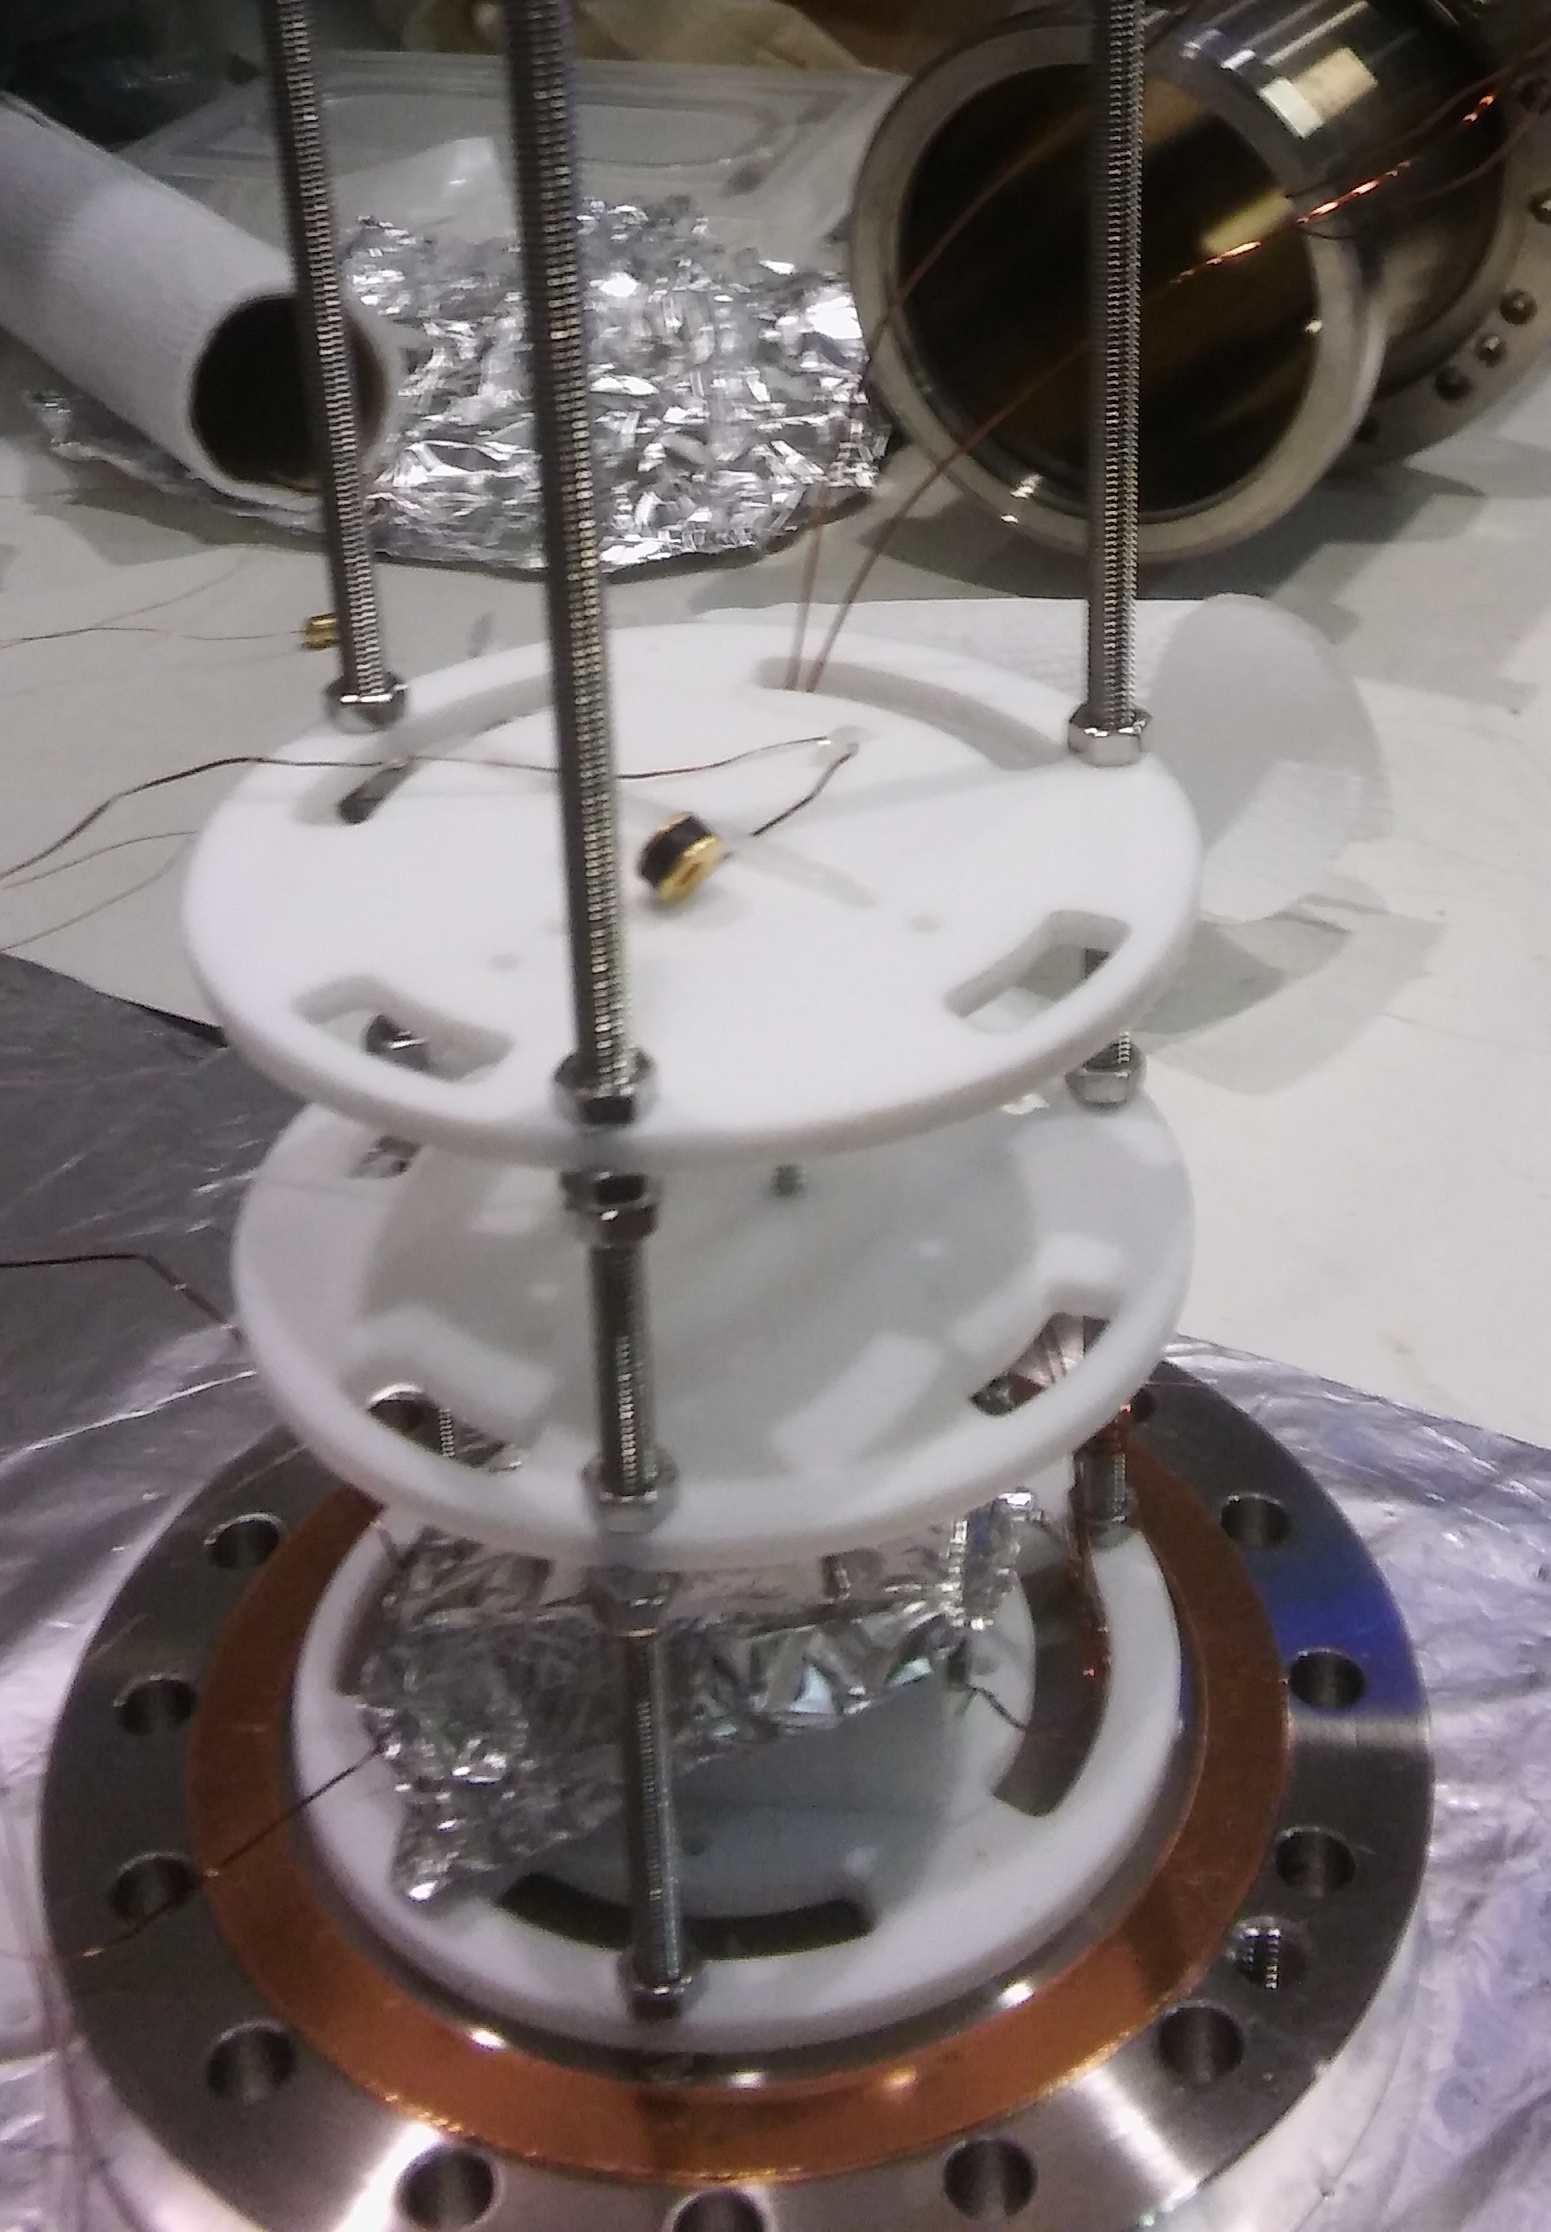
\includegraphics[height=6cm]{pds-tgm_1} \quad
%	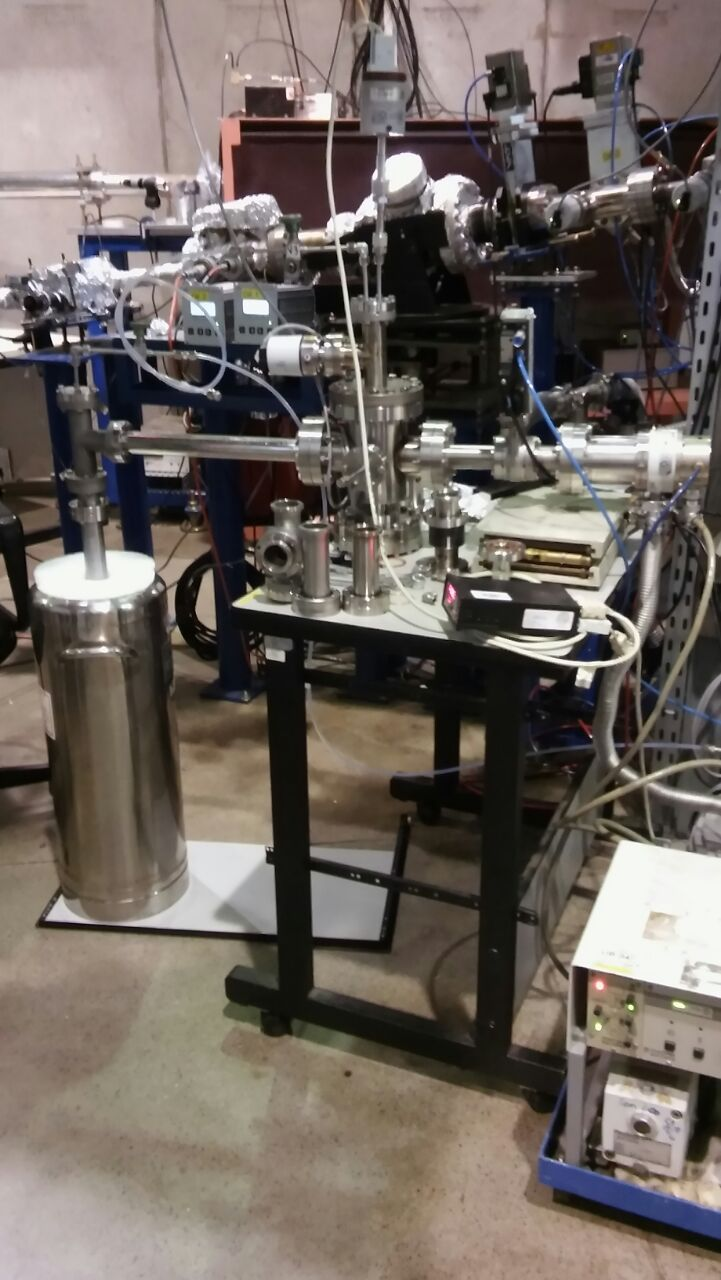
\includegraphics[height=6cm]{pds-tgm_30}\quad
%	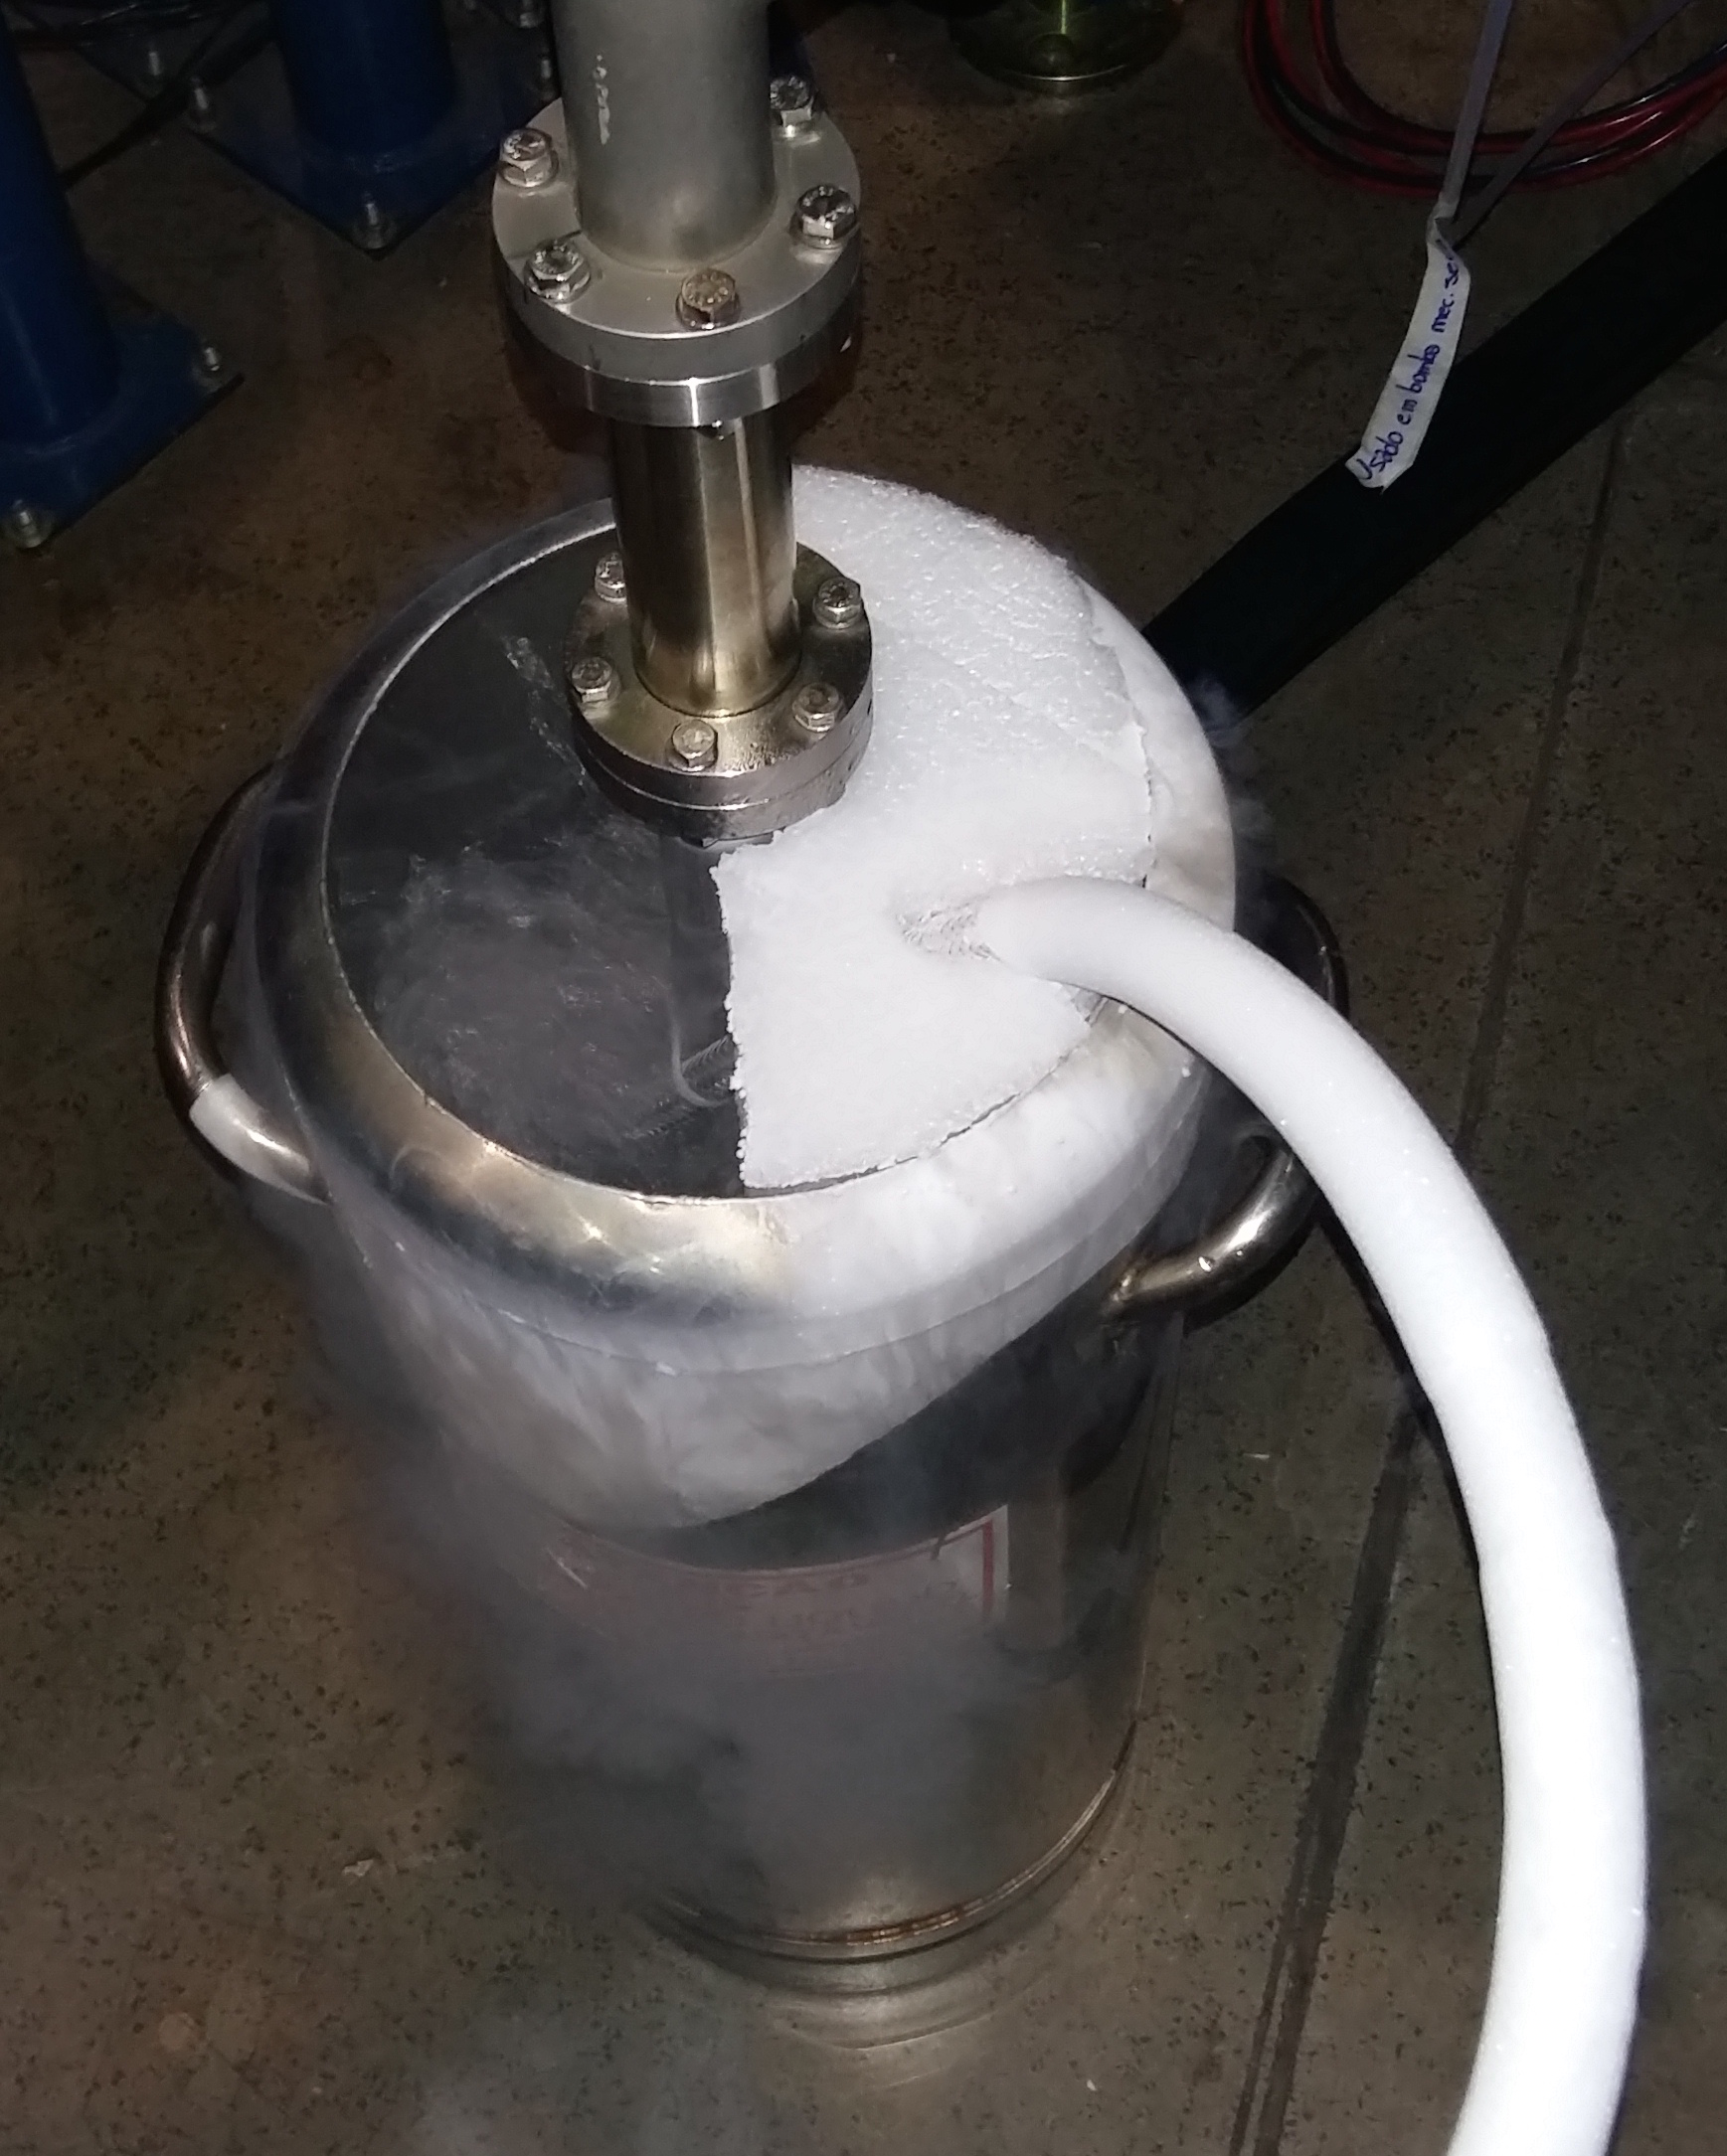
\includegraphics[height=6cm]{pds-tgm_0}
%\end{dunefigure}

The detection efficiency of the ARAPUCA was calculated by determining the number of detected photoelectrons corresponding to the end point of the $\alpha$ spectrum and comparing that with the expected number of photons impinging on the acceptance window for that energy value (\SI{4.267}{MeV}).  This calculation depends only on known properties of \lar and on the solid angle subtended by the ARAPUCA window. A detection efficiency at the level of 1.8\%  was measured, consistent with \dword{mc} expectations for this configuration~\cite{Marinho:2018doi}.


%%%%%%%%%%%%%%%%%%%%%%%%%%%%%%%%%
\subsubsection{Multi-cell Measurements}
%\metainfo{New content: Gustavo}

%%%%%%%  
%The TallBo facility at Fermilab provides a \SI{450}{liter} capacity cryostat with \SI{56}{cm} inner diameter and up to a \SI{183}{cm} liquid depth that accommodates  up to three different PD modules with dimensions \todo{how different?} close to the real ones.

Eight ARAPUCA cells with filters from different manufacturers, different reflectors, and different dimensions were tested in early 2017 using the \dword{tallbo} facility at Fermilab.  
%Per Gustavo 12/4/18 
The ARAPUCA cells each contained two \SI{6}{mm} $\times$ \SI{6}{mm} SensL \dwords{sipm}. 
An $^{241}$Am source, mounted on a movable holder that allowed placement in front of each prototype, provided the scintillation light. The measured detection efficiencies of these ARAPUCAs ranged from 0.4\% to 1.0\%.

In late 2017 we measured an array of eight ARAPUCA cells together with two reference bars of a double-shift light guide design. An array of counters on opposite sides of the cryostat formed a cosmic ray trigger. 
Two configurations of trigger selected through-going muons that pass through the cryostat at mean angles ranging from $36^{\circ} $ to $70^{\circ} $ from vertical, and from $65^{\circ} $ to $90^{\circ} $ from vertical, with each angle accepting approximately $\pm 3^{\circ}$ about the mean. The possible array combination along with the muons flux angular dependence produces a non-symmetrical distribution of the muons in zenith angle: for the first configuration the mean angle was $46^{\circ}$ and for the second configuration $75^{\circ}$; 90\% of events are in a range of $\pm 10^{\circ}$ from the means value in both cases.
The expected light production was adjusted for the crossing angle but the angular acceptance of the trigger introduces a spread in the expected number of photos of about 10\% (between 6\% and 15\% depending on the track).

% The so-called ``hi-low'' trigger selected through-going muons at a few degrees away from vertical.
%\fixme{rjw what was the range of angles for the Hi-Low CR selection?}
%\fixme{Gustavo to include updates from recent TallBo analysis.}
% from Gustavo; edited down by rjw
%\subsection{Efficiency analysis}
%\textit{\it TallBo Measurement Efficiency analysis}

We define the detector efficiency as the ratio between the number of measured photons and the estimated number of photons arriving at each ARAPUCA:
%\begin{equation}
$\mathcal{R}_{i}=\frac{PE_i}{PH_i}$.
%\end{equation} 
In addition to this metric, the ratio between the total number of photoelectrons measured in all the ARAPUCAs divided by the total number of photons landing on them is also calculated. 
%\begin{equation}
$\mathcal{R}_{TOT}=\frac{\sum_{i=1}^8PE_i}{\sum_{i=1}^8PH_i}$
%\end{equation} 

% Simplify to just the one reported on. 
%Three kinds of analyses were performed on these datasets and produced similar results:
%(1)  a log-normal fit above the ratio values $\mathcal{R}_{TOT} $ and $\mathcal{R}_{i}$, taking into account the median of the distribution; 
%(2) a robust statistic procedure, getting the median of the data set cleaned out by the outliers given by the median absolute deviation (\cite{stats-rous+hub}; %\{RousseeuwHubert_RobustStatisticsForOutlierDetection_WIREs_2011 should be cited}
%Rousseeuw Peter J., Hubert Mia. Robust statistics for outlier detection. WIREs Data Mining Knowl Discov 2011, 1: 73-79. doi: 10.1002/widm.2   (Online http://wires.wiley.com/WileyCDA/WiresArticle/wisId-WIDM2.html)
% email sent to Luke Corwin to see if he can make the entries in the bib file

%A data set of selected events for each of the two trigger configurations was found.
Using the trigger information, muons with a path passing entirely in front of the ARAPUCA cells windows were selected.
A bootstrap procedure \cite{stats-diaconis-efron-1983} was used to evaluate the average $\mathcal{R}_{TOT} $ and $\mathcal{R}_{i}$ values on a reduced selection of events for which there were a strong correlation in the response of each ARAPUCA, relying on the Pearson correlation coefficient condition: $r >0.7$. Two other analysis methods were used that gave compatible results. 

%Here are reported only the ones given by the third procedure since the range of errors is the smaller. 
%\fixme{Computer intensive methods in statistic by Persi Diaconis and Bradley Efron. Technical Report N.83 Jan 1983. Stanford University California    should be cited --- is this citation for the Boostrap method? -- yes per Dante}

Figure~\ref{fig:pds-tallbo-arapuca} displays the mean of the set of average values obtained from the measured photon distributions using the bootstrap procedure.
The green points are for muons with a zenith angle of $\sim 46^{\circ}$ and the purple points are muons centered on $\sim 75^{\circ}$.
The first three ARAPUCAs were not used in the low angle configuration since they were far enough from the volume where the tracks were triggered that they were exposed to only a few hundred photons so the number of measured photons were of the order of 1 - 10 and the ratio estimation had a large statistical fluctuation. 
 
The $x$-axis is the ARAPUCA number, except number 0 labels the results for all cells combined; the $y$-axis is the detection efficiency. The two configuration are in agreement after the energy deposit value has been corrected for track angle: \SI{2.2}{MeV/cm} to $\sim\,$\SI{3.0}{MeV/cm} passing from the $\sim 46^{\circ}$ to $\sim 75^{\circ}$ configuration, respectively.
The horizontal configuration shows larger error because the total number of events was much less than the higher angle configuration.

The TallBo experiment showed that ARAPUCAs with only four \dwords{mppc} %with 
covering a total area of \SI{1.44}{cm^2} and a photon collection area of \SI{80}{cm^2} achieved close to 1\% absolute efficiency (the range of values for the eight ARAPUCA cells is 0.72\%--0.80\%). The effective ARAPUCA gain is about 4.5 times the photosensor area.

\begin{dunefigure}[ARAPUCA TallBo measurements.]
 {fig:pds-tallbo-arapuca}
 {Average values of the set of mean values obtained with the bootstrap procedure for each ARAPUCA.
The green points come from the configuration for muons with a zenith angle of $\sim 46^{\circ}$ and purple points for $\sim 75^{\circ}$ . Number 0 is relative to the total ratio, the others are the ARAPUCA
numbers.}
%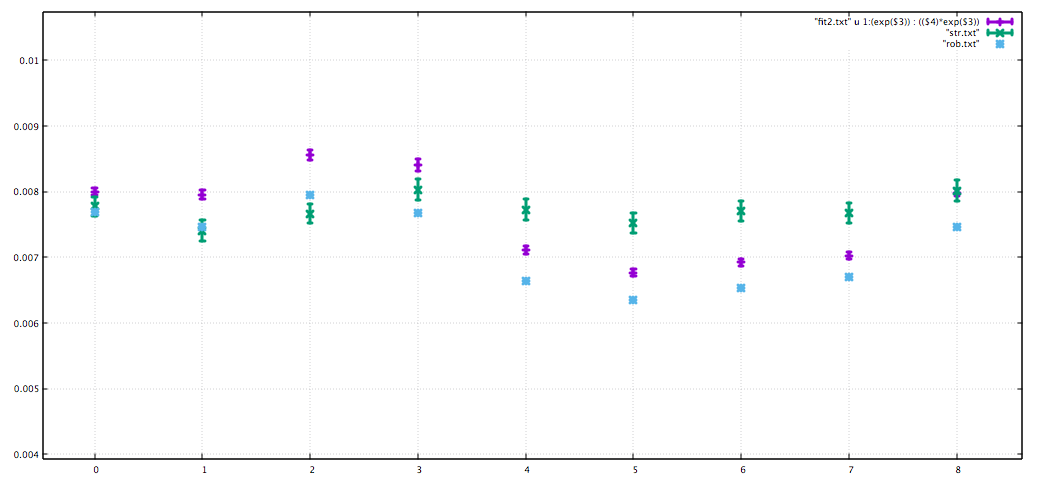
\includegraphics[angle=0,width=8.4cm,height=6cm]{pds-tallbo-arapuca-trepl.png}
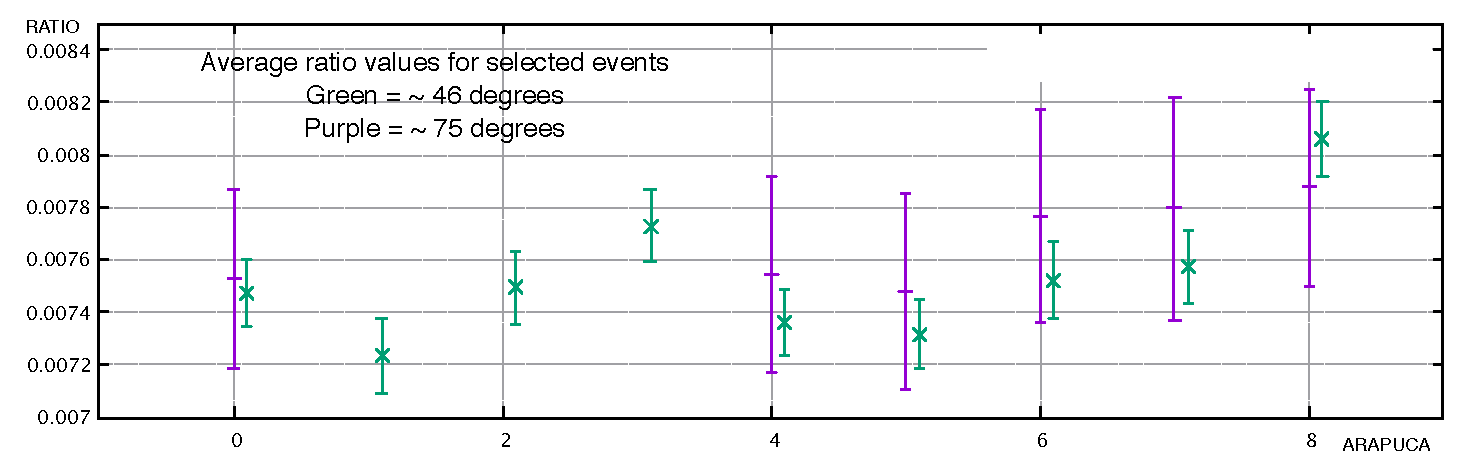
\includegraphics[angle=0,height=3cm]{graphics/pds-arapuca_ratio.pdf}
\end{dunefigure}


\subsubsection{Photosensors and Active Ganging}
\label{sec:pds-valid-ganging}
%\metainfo{Content: Gustavo}
%\fixme{11/29/18? Zelimir added this subsection, with Gustavo's material}

As described in Section~\ref{sec:pds-design-ganging}, the active ganging of \dwords{sipm}  aims to increase the active photo-detecting area while keeping the number of readout channels at a reasonable number. 
%Even when the ARAPUCA has a gain in detector sensitive area, the internal reflectivity of the ARAPUCA is not 100\%, hence more than a single photosensor per ARAPUCA is needed to keep a good photon collection efficiency. 
Several active ganging detectors were designed and tested during 2017-2018. 
The systems were based on an active summing node working in the \lar near the photosensors. Several incarnations of the cold summing node were designed and tested using SensL and Hamamatsu \dwords{sipm} %\fixme{\dwords{mppc}?} -- rjw SiPM is the generic name, MPPC is specific to Hamamatsu  %and also 
as were several types of operational amplifiers (OpAmps). 
Some of these designs were tested, validated and successfully contributed to the March and November 2017 TallBo experiments.  
We describe here only the most recent design that demonstrated that 48 Hamamatsu \dwords{mppc} in the baseline design can be ganged together on a single differential output with excellent signal performance, low noise and low power dissipation.

Figure~\ref{fig:fig-pds-gang-1}(left) shows a matrix array of 72 \dwords{mppc} organized as 12 rows of six \dwords{mppc} each. 
The six \dwords{mppc} per row are connected in parallel, giving a total output capacitance of \SI{7.8}{nF}. The 12 rows are connected to the summing node of an OpAmp THS4131, as sketched in Figure~\ref{fig:fig-pds-gang-1}(right). 
Since the DUNE baseline design is based on 48 \dwords{mppc}/ARAPUCA module, only eight rows of six were used for the tests. 
The performance of the cold summing electronics was done by illuminating the \dword{mppc} array with an LED and digitizing the output with a high-speed oscilloscope and with the \dword{ssp} readout electronics (see Section~\ref{sec:ssp-protodune-electronics}).
As shown in Figure~\ref{fig:fig-pds-gang-2}, the mean signal shows a rise time of \SI{60}{ns} and a recovery time of \SI{660}{ns}, well within the DUNE \dword{pd} specifications. %requirements.

\begin{dunefigure}[Photosensors signal ganging scheme.]
 {fig:fig-pds-gang-1}
 {Summing board with a total of 72 \dwords{mppc} used to demonstrate the optimal combination of passive and active ganging with 48 Hamamatsu \SI{6}{mm}$\times$\SI{6}{mm} \dwords{mppc} (left).  Schematics of summing circuit with an OpAmp THS4131 (right).}
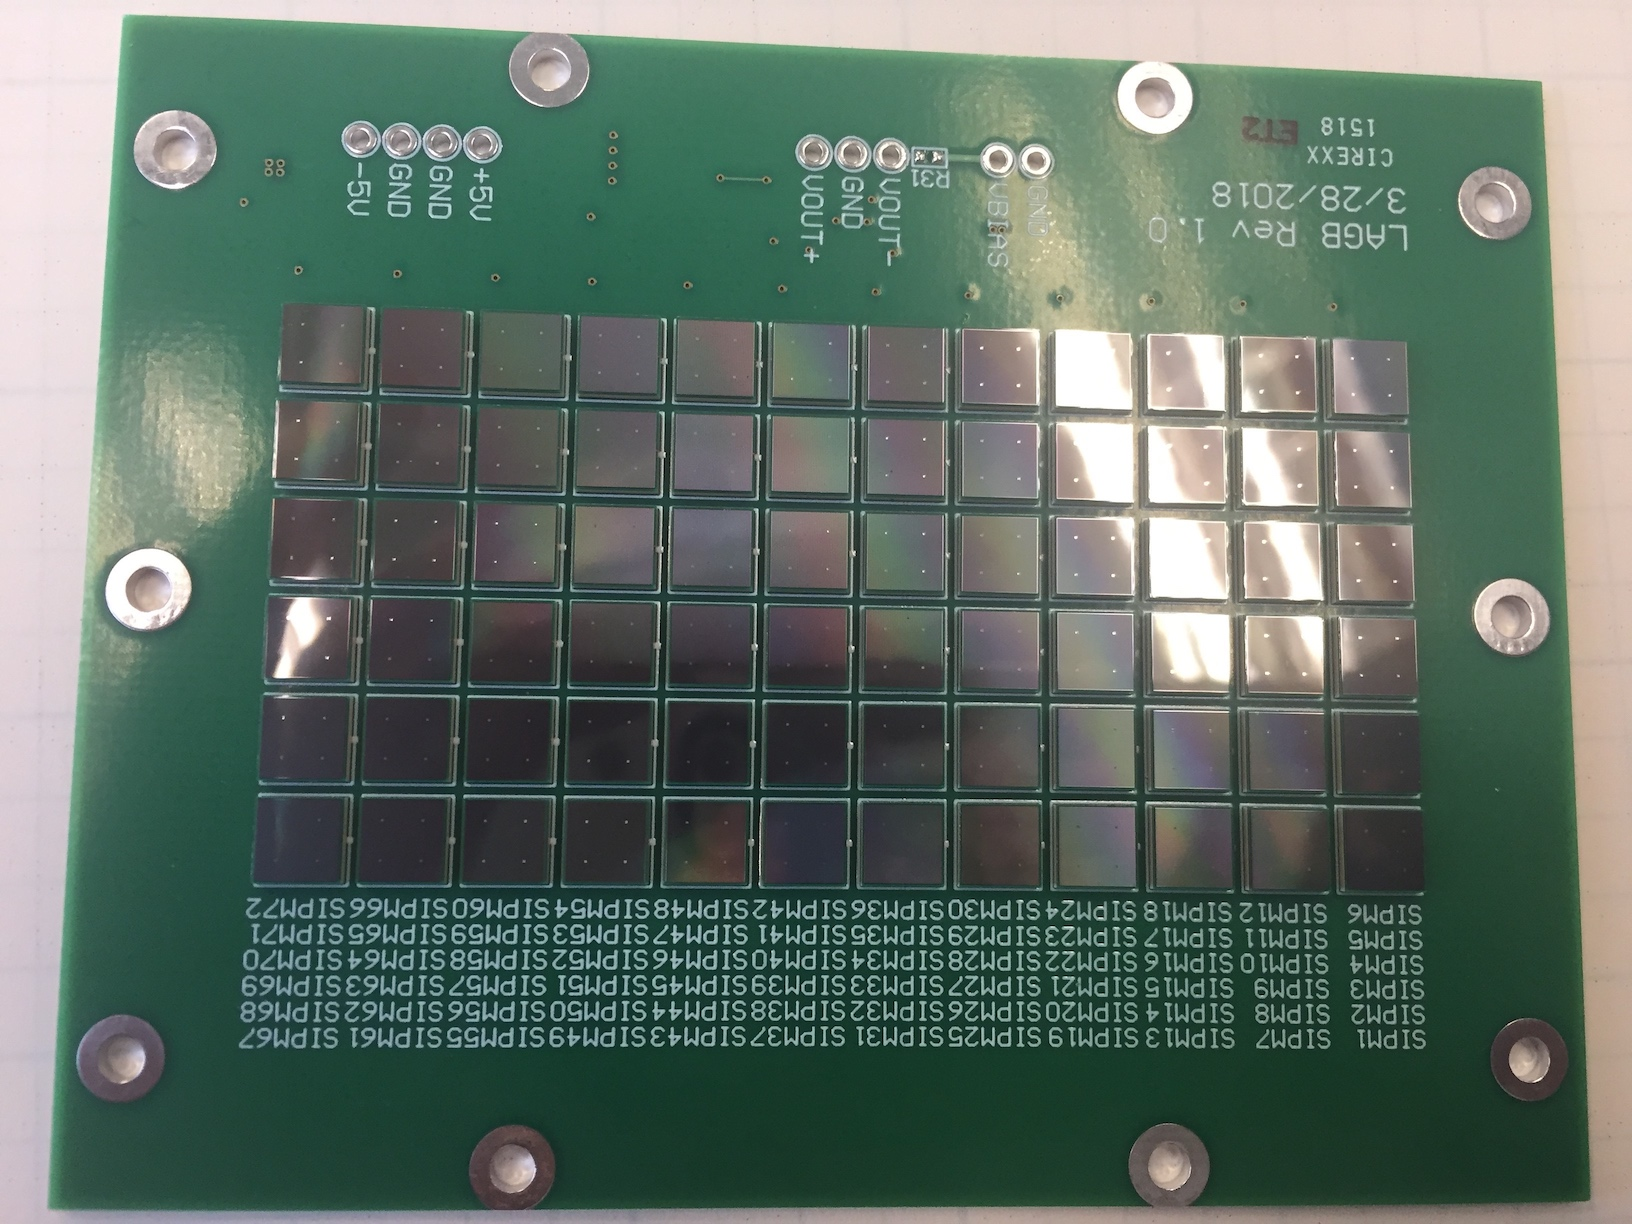
\includegraphics[height=6cm]{graphics/pds_gang_fig1.jpg}
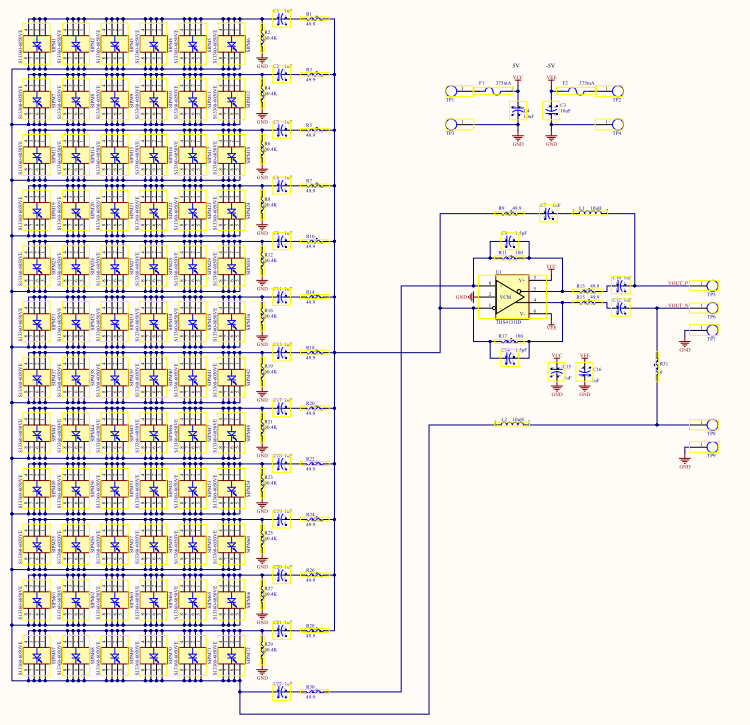
\includegraphics[height=6cm]{graphics/pds_gang_fig2.png}
\end{dunefigure}

\begin{dunefigure}[Photosensors signal ganging with 48 \dwords{sipm}.]
 {fig:fig-pds-gang-2}
 {Waveform signal from 48 \dwords{mppc}/ARAPUCA module, summed with OpAmp THS4131, and digitized with the \dword{ssp} frontend board.}
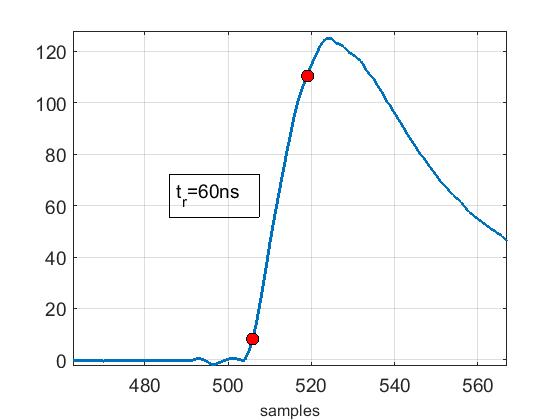
\includegraphics[width=.5\textwidth]{pds-gang-rise_time.jpg}
\end{dunefigure}

\begin{dunefigure}[Photoelectron peaks from 48 ganged \dwords{mppc}.]
 {fig:fig-pds-gang-3}
 {Photoelectron peaks from 48 ganged \dwords{mppc}, collected in liquid nitrogen at 45 Volt bias (left) and at 47 Volt bias (right).}
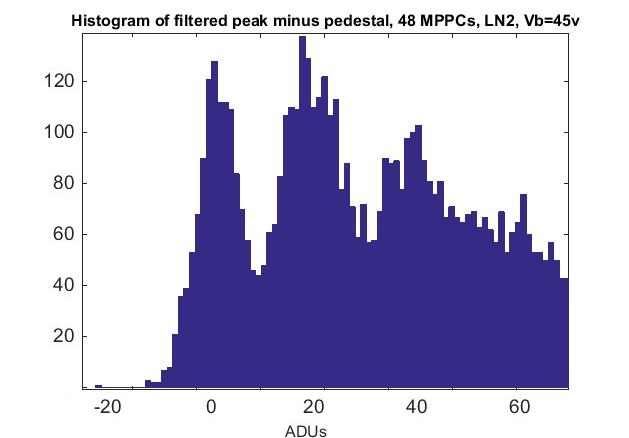
\includegraphics[height=4.5cm]{graphics/pds-gang48-45v.jpg}
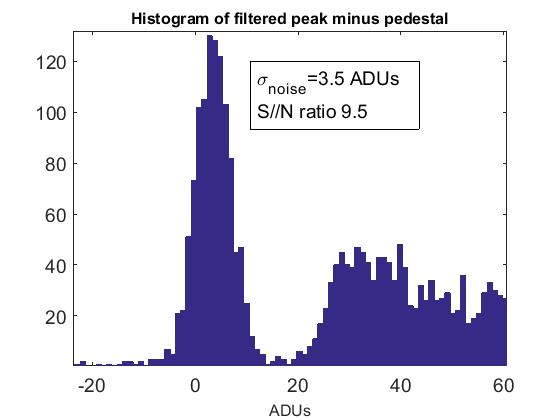
\includegraphics[height=4.5cm]{graphics/pds-gang48-47v.jpg}
\end{dunefigure}
\fixme{Need larger text on the figures}

Figure~\ref{fig:fig-pds-gang-3} shows a histogram of light collection in the array for a bias voltage equivalent to 2 volts above the mean breakdown voltage. Since there are 48 \dwords{mppc} in the array, and a single common bias, there is a spread in the allowed gains. Even when the Hamamatsu \dwords{mppc} have a small spread in breakdown voltages, that spread is enough to smear the peaks in the histogram. It is worth noting the difference between noise and gain spread. The circuit noise can be measured as FWHM or RMS around the 0 PE signal (3.5 ADC counts in the figure). The first PE peak is at 33 ADC counts, resulting in an optimal signal to noise ratio of about 10.

Since the breakdown voltage of the \dwords{mppc} is specified by the manufacturer, for the DUNE experiment the gain spread can be reduced by picking groups of 48 \dwords{mppc} with similar breakdown values for each module. The differential output of the cold electronics impedance is matched to the readout electronics and able to reject more than \SI{60}{dB} of common mode noise. This is particularly important since the \dwords{mppc} and output wiring are inside a high voltage TPC. The timing properties of the 48 ganged electronics were also measured 
in LAr using a Am-241 alpha source. 
Figure~\ref{fig:fig-pds-gang-4} shows the time walk for a constant discrimination threshold which, 
%Figure~\ref{fig:fig-pds-gang-5} shows that, 
as expected, is not a linear function of the signal height. The error distribution, which is not Gaussian, has a FWHM of \SI{80}{ns}. This value is well within the DUNE specification (Table~\ref{tab:spec:time-resolution}).

\begin{dunefigure}[Time walk from 48 ganged \dwords{mppc}.]
 {fig:fig-pds-gang-4}
 {Time walk from 48 ganged \dwords{mppc} measured at the constant discrimination threshold with \dword{ssp} board.}
%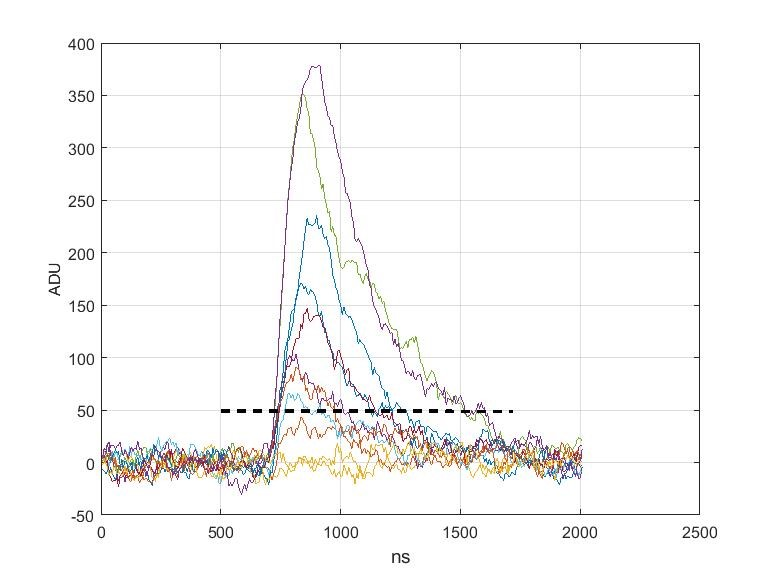
\includegraphics[angle=0,width=8.4cm,height=4cm]{graphics/pds_gang_fig6.jpg}
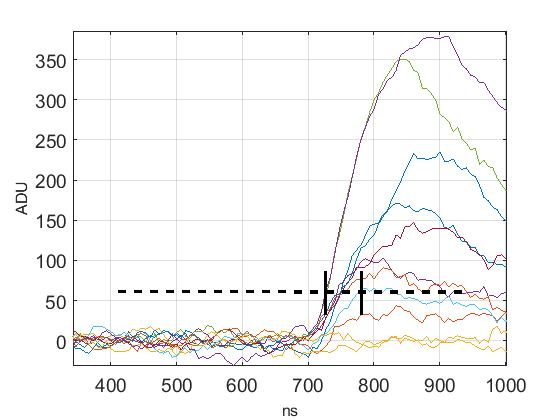
\includegraphics[height=4.5cm]{graphics/pds-gang-time_walk.jpg}
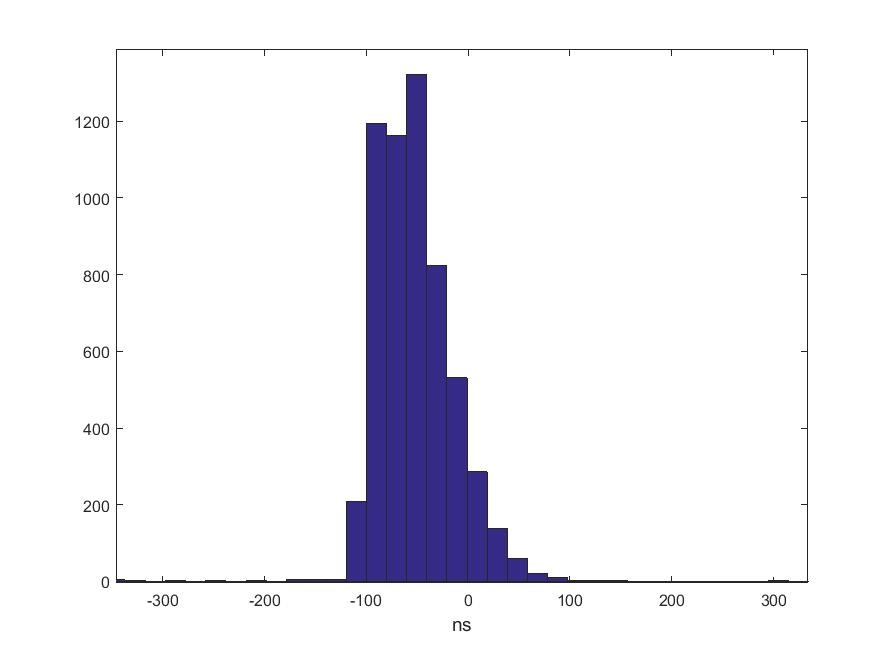
\includegraphics[height=4.5cm]{graphics/pds_gang_fig8.jpg}
\end{dunefigure}

%Figure~\ref{fig:fig-pds-gang-5}  shows that, as expected, the time-walk is not a linear function of the signal height. The error distribution is not Gaussian. 
%The FWHM is 80 ns. This value meets DUNE physics requirements.

%\begin{dunefigure}
% {fig:fig-pds-gang-4}
% {Distribution of the time walk from from 48 \dwords{mppc}/ARAPUCA module.}
%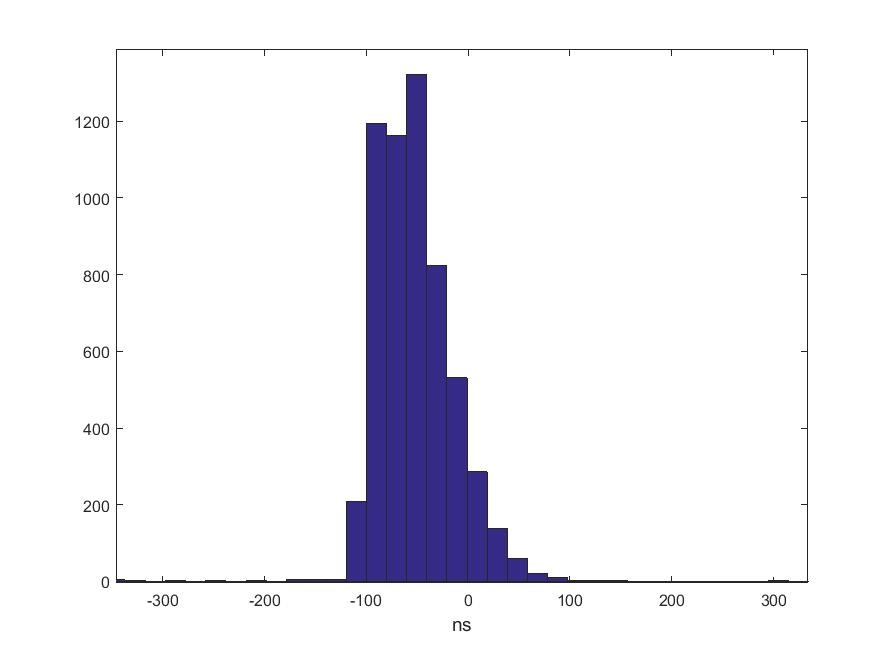
\includegraphics[angle=0,height=4cm]{graphics/pds_gang_fig8.jpg}
%\end{dunefigure}

%Primarily this section is a summary of the active ganging studies, but is also effectively a report of the \dwords{mppc}.

%% Short section on Mu2e electronics with the active ganging studies 
% From Josh S 11/28/18
%\subsection{Mu2e Electronics Validation Tests, Completed and Planned}
\textit{Mu2e Electronics Validation}
%\fixme{Gustavo/Josh need to blend this Mu2e text with the active ganging studies text.}
The Mu2e electronics have undergone a number of end-to-end warm and cold tests to demonstrate single-photon sensitivity in various parallel/series ganging and \dword{sipm}/\dword{mppc} configurations. Here we summarize the results with the 72-\dword{mppc} active ganging array described in Section~\ref{sec:pds-valid-ganging}
%(Vb = 47.2 V; each of 12~rows of 6x6 mm$^2$ Hamamatsu S13360-6050VE \dwords{mppc} in %parallel, with total capacitance of 7.8 nF per row) 
at liquid nitrogen temperatures. 
%This active ganging system, discussed in Section~\ref{}, is designed to mimic the arrangement envisioned for DUNE, although the DUNE \dword{pd} active ganging scheme will feature 48~\dwords{mppc} rather than 78. 
A balun is used to convert from the differential \dword{mppc} array output to the single-ended \dword{feb}. The data represent triggers in time with an LED flasher, with samples taken every 12.5~ns for the length of the readout window ($\sim$3~$\mu$s in this case). Figure~\ref{fig:pds-board-balun-adc} shows the system used and a histogram of the maximum ADC value during each trigger window. The first peak above zero represents noise and the second peak represents a one-PE signal. The signal to noise from these tests was measured to be 4, determined by the ratio of the single photon peak (20 ADC, after subtracting the noise peak) to the spread in the noise ($\sigma_{noise}$ = 5~ADC) for direct comparison to the \dwords{ssp} (S/N = 5).

\begin{dunefigure}[Readout of 72-\dword{mppc} active ganging array with the Mu2e electronics readout board.]
{fig:pds-board-balun-adc}
{The Mu2e electronics readout board was used to read out a 72-\dword{mppc} active ganging array (V$_b$ = \SI{47.2}{V}) (left). The maximum ADC results are shown, with the first and second peaks representing 0 and 1~photoelectron signals (right).}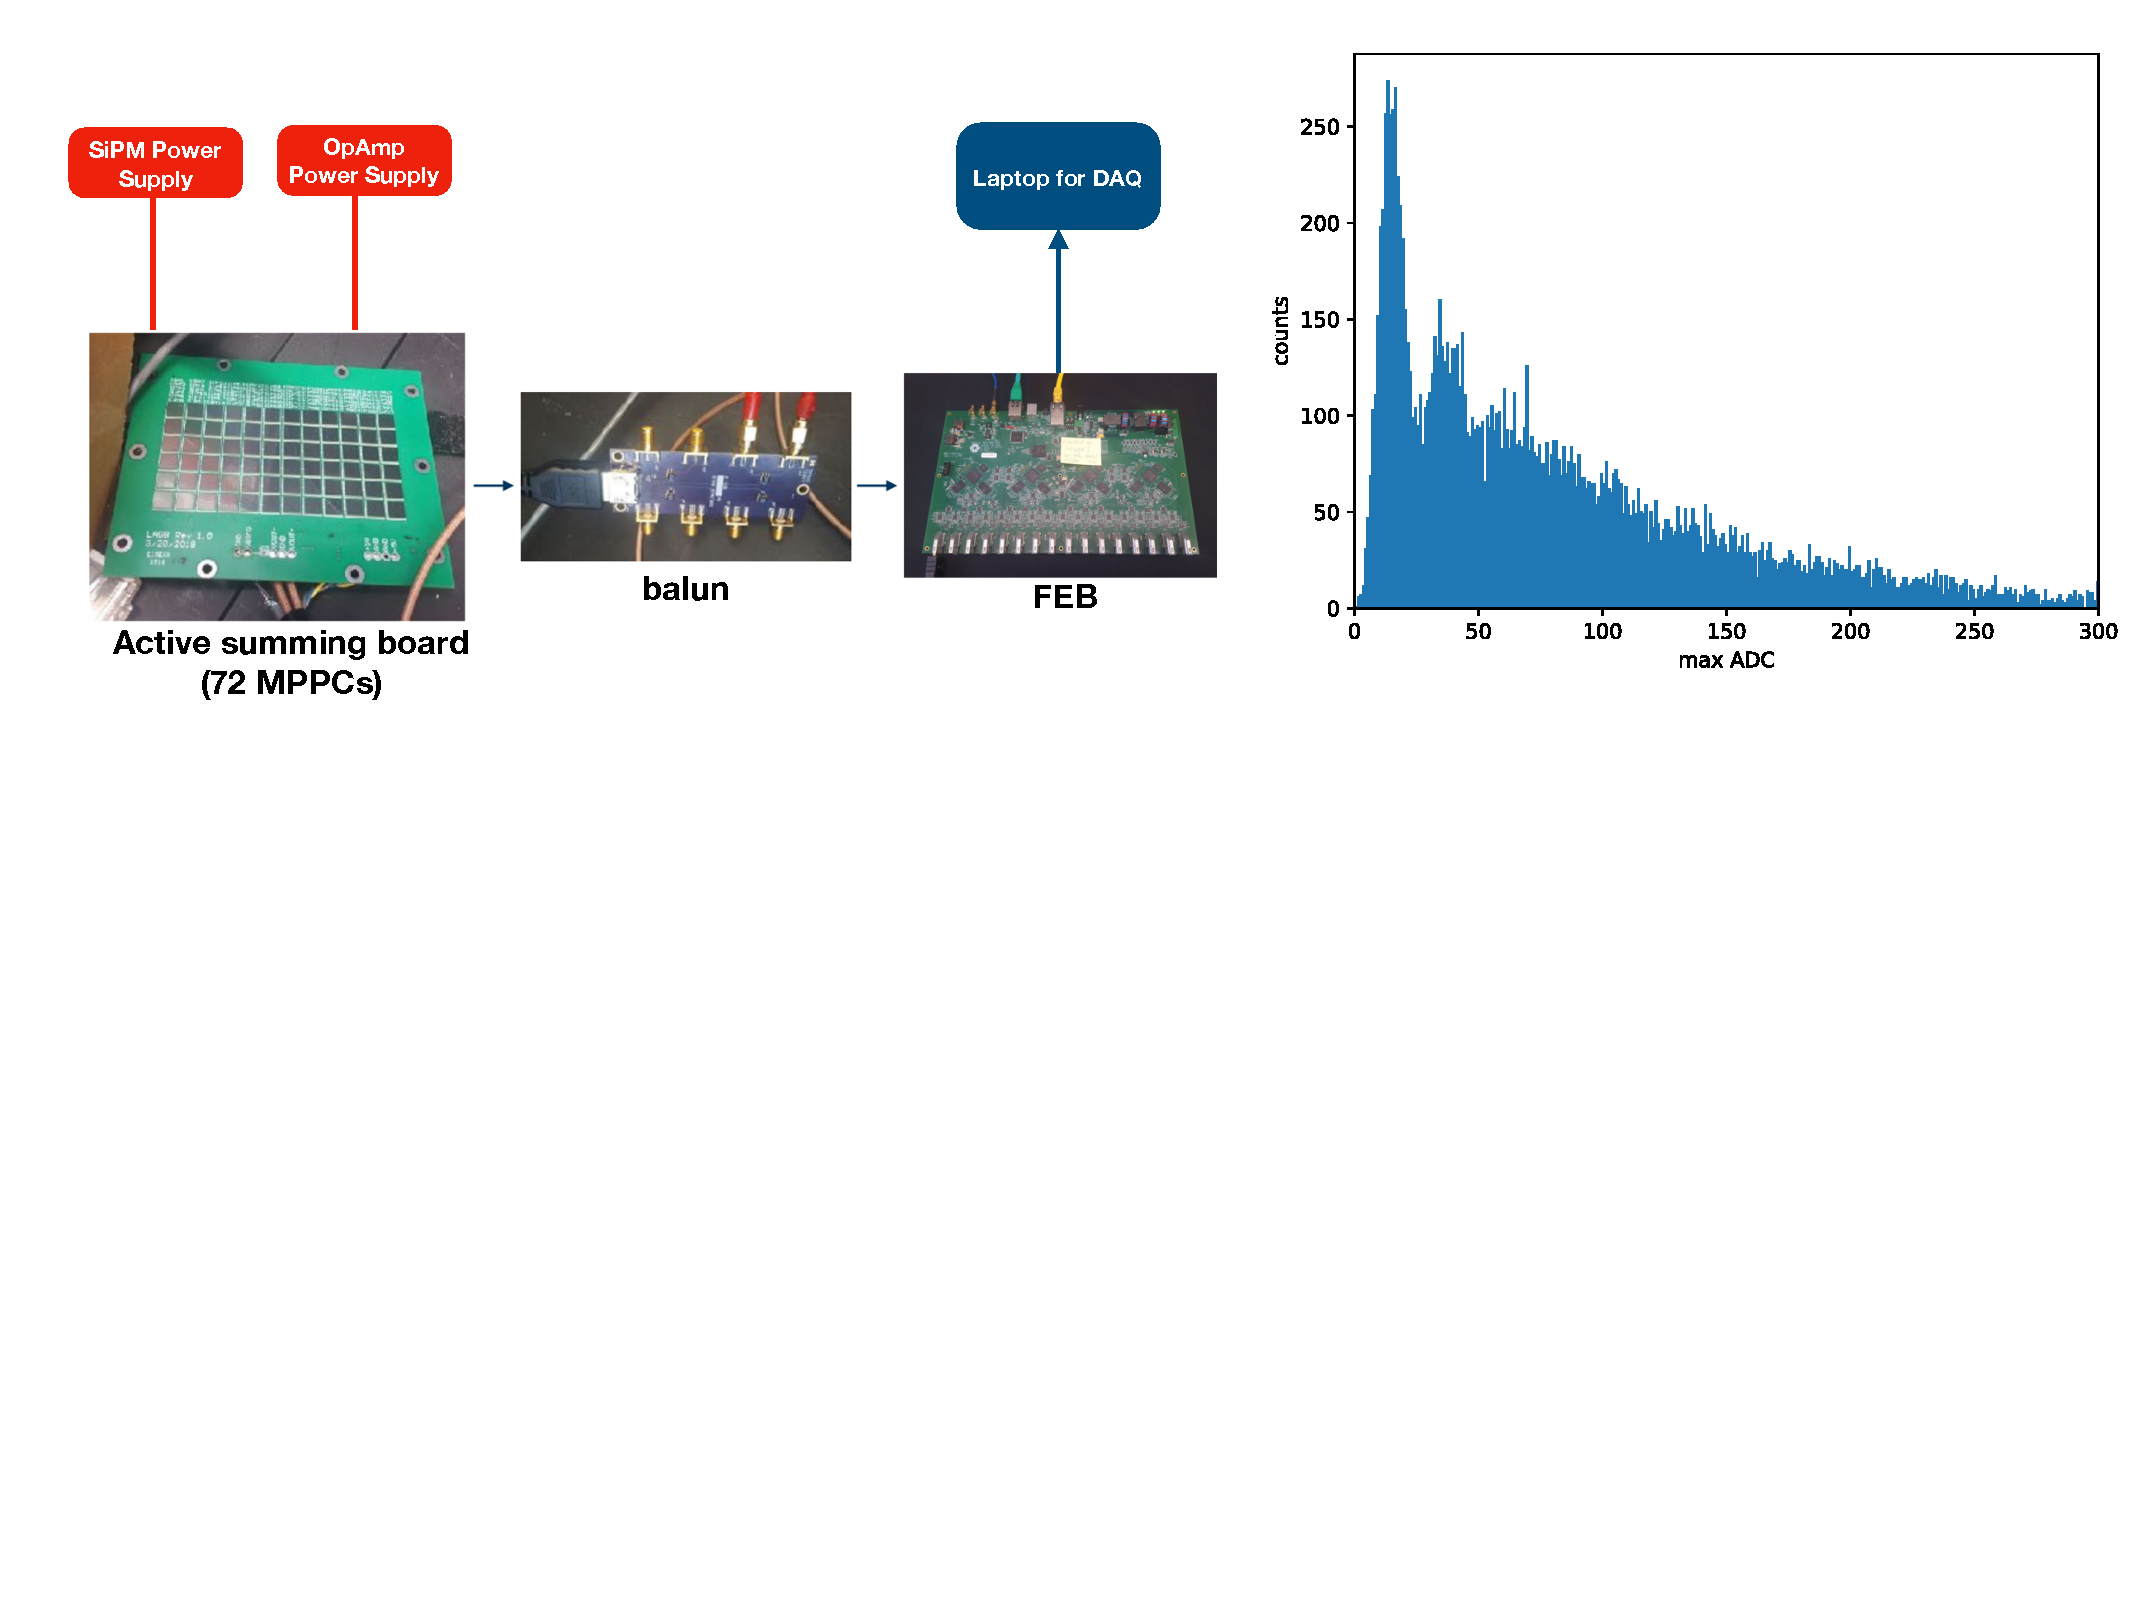
\includegraphics[height=4.8in]{pds-board-balun-adc} 
\vspace{-7.0cm}
\end{dunefigure}


%%%%%%%%%%%%%%%%%%%%%%%%%%%%%%%%%%%%%%%%%%%%%%%
% rjw 11/23/18 add section headings for the major sources of ARAPUCA information to come.
%>>>> ProtoDUNE
%%%%%%%%%%%%%%%
\subsection{\dword{pdsp}}
%\metainfo{\color{blue} Content: Mualem}

The most comprehensive set of data on the \dword{sarapu} will come from the fully instrumented modules in the \dword{pdsp} experiment~\cite{Abi:2017aow} that completed first beam running in November \num{2018}. 
Since \dword{pdsp} will remain filled with \lar for much of the CERN long-shutdown we will also have a long-term cold test of full-scale \dword{pd} modules for the first time so it may be possible to quantify any deterioration in their performance.
%such as the loss of \dword{tpb} from the coating noted previously. 
%More broadly, aging effects in various detectors technologies, such as scintillator and \dwords{pmt}, are well documented, and knowledge of such effects is required at the design stage so that the photon detection performance will meet minimum requirements for the whole life of the experiment.


Three photon collector designs are present in \dword{pdsp}: \num{29} double-shift guides, \num{29} dip-coated guides, and two \dword{sarapu} arrays. 
The TPC provides precise reconstruction in \threed of the track of any ionizing event inside the active volume and matching the track with the associated light signal will enable an accurate comparison of the relative detection efficiencies of the different \dword{pd} modules. 
The large number of modules and independent channels that record each event can be used to constrain the propagation parameters of the \lar that regulate \dword{vuv} light propagation in the simulation and are poorly determined in the literature. %such as Rayleigh scattering length
In principle, absolute calculations are also possible using \dword{mc} simulations.
The absolute precision of this approach may be limited by the precision of the constraints on the parameters, but will result in a consistent simulation constrained by actual measurements. 

The first large-scale implementation of an \dword{sarapu} module, in \dword{pdsp}, is composed of an array of sixteen cells.
%The \dword{pdsp} ARAPUCA design collects light from one side of the box through an optical window formed  
%by a dichroic filter deposited with a layer of pTP\footnote{p-TerPhenyl,  supplier: Sigma-Aldrich\textregistered.}
%wavelength shifter on the external surface that shifts the incident \dword{vuv} light to a near-visible frequency able to pass through the filter plate to the interior of the box.  
The \dword{sarapu} design collects light from one side of the box through an optical window formed by a dichroic filter deposited with a layer of pTP\footnote{p-TerPhenyl, supplier: Sigma-Aldrich\textregistered.}
% https://www.sigmaaldrich.com/catalog/substance/pterphenyl230309294411.} 
wavelength shifter on the external surface. This shifts the incident \dword{vuv} light to a near-visible frequency that is able to pass through the filter plate to the interior of the box.  

In the \dword{pdsp} version of \dword{sarapu}, the inner surface of the box opposite the window houses an array of \dwords{sipm} that covers a small fraction of the area of the window (2.8-5.6\%), surrounded by a foil of a highly reflective material coated with a second wavelength shifter, \dword{tpb}. The \dword{tpb} converts the light passing through the filter to a wavelength that is reflected by the filter. It has been shown in simulation and in prototypes that a large fraction of these trapped photons, reflecting from the filter and the lined walls of the box, will eventually fall on a \dword{sipm} and be detected.

Two \dword{sarapu} arrays have been operated in \dword{pdsp}. The first is installed in the \dword{apa} \#3 in the fourth position from the top.  This is near the level the beam particles enter this drift volume in order to illuminate it and the surrounding modules with a significant amount of light from each beam particle interaction.
The second is installed in the \dword{apa} \#6 in the 6th position from the top.  This module does not see significant light from beam events, but it is also surrounded by light guide modules, signals from these will help to constrain the light that the module is detecting from each interaction.

%\fixme{LMM Do we want to make SiPM->MPPC in this section?  All are MPPCs}
% I made the conversion sipm->MPPC
Each \dword{pdsp} \dword{sarapu} module array is composed of sixteen cells, where each cell is an \dword{sarapu} box with dimensions of \SI{8}{cm} $\times$ \SI{10}{cm}; half of the cells have twelve \dwords{mppc} installed on the bottom side of the cell and  half have six \dwords{mppc}. The \dwords{mppc} have active dimensions \SI{0.6}{cm}$\times$\SI{0.6}{cm} and account for 5.6\% (\num{12} \dwords{mppc}) or \num{2.8}\% (\num{6} \dwords{mppc}) of the area of the window (\SI{7.8}{cm}$\times$\SI{9.8}{cm}).
The \dwords{mppc}  are passively ganged together, so that only one readout channel is needed for each \dword{sarapu} grouping of \num{12} \dwords{mppc} (the boxes with six \dwords{mppc} are ganged together to form \num{12}-\dword{mppc} units) so a total of \num{12} channels is required per module. 
%Studies are underway to investigate active ganging that would permit combining signals from multiple boxes, as required to reduce the number of electronics channels and cables under the working assumption that the \single \dword{pds} is restricted to four readout channels per \dword{pd} module. 
The total width of a module is \SI{9.6}{cm}, while the active width of an \dword{sarapu} is \SI{7.8}{cm}, the length is the same as the light guide modules (\SI{210}{cm})\footnote{Since \dword{pdsp} was constructed, the slot opening in the \dword{apa} opening for \dword{pd} module installation has been enlarged allowing for a module with larger collection area}.
An \dword{sarapu} array during assembly is shown in Figure~\ref{fig:sarapuca_array_prod} during the assembly; the array installed in \dword{pdsp} is shown in Figure~\ref{fig:arapuca-protodune}. If the \dword{sarapu} cells achieved the same detection efficiency as earlier prototypes (1.8\%), the effective area of an \dword{sarapu} module will be approximately \SI{23}{cm$^2$}.

\begin{dunefigure}[Photo of ARAPUCA module prototype assembly.]{fig:sarapuca_array_prod}
{ProtoDUNE ARAPUCA module being assembled in a class 100,000 clean area.  Front face of assembled module (left) shows the 16 coated dichroic filter plates.  Assembly photos show the reflective rear side (top right) and inner coated surface (right bottom) of Vikuiti reflective foils.  Note the cutouts in foil for \dword{mppc} active area.}
	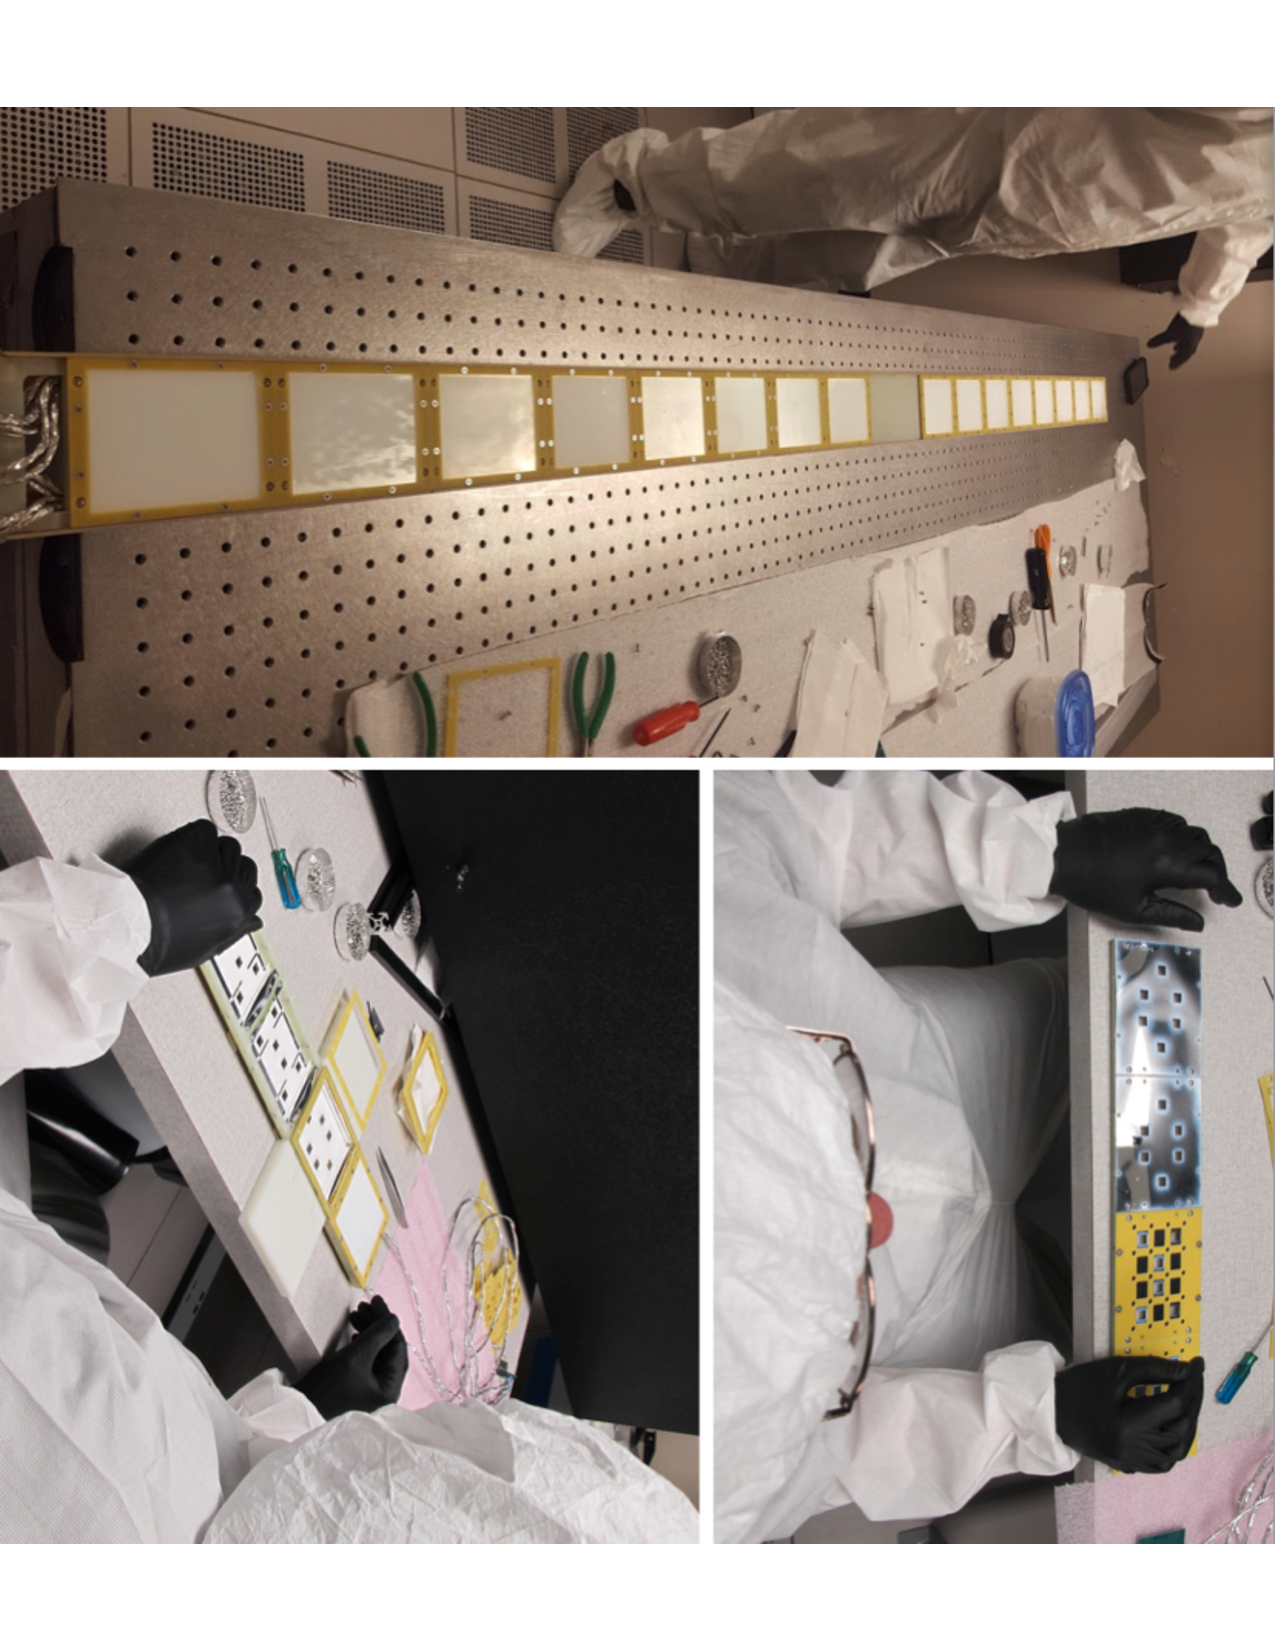
\includegraphics[angle=90,width=0.75\columnwidth]{pds-pdune-arapuca-assby}
\end{dunefigure}

%\begin{dunefigure}[\dword{sarapu} array during assembly.]{fig:sarapuca_array_prod}
%{\dword{sarapu} array during assembly.}
%{\dword{sarapu} array for \dword{pdsp} during assembly. (\dwords{sipm} are visible in the sixteen cells before the installation of reflecting foils, coated filter windows, and readout cabling) (Left); ARAPUCA array in \dword{pdsp} (Right).} 
%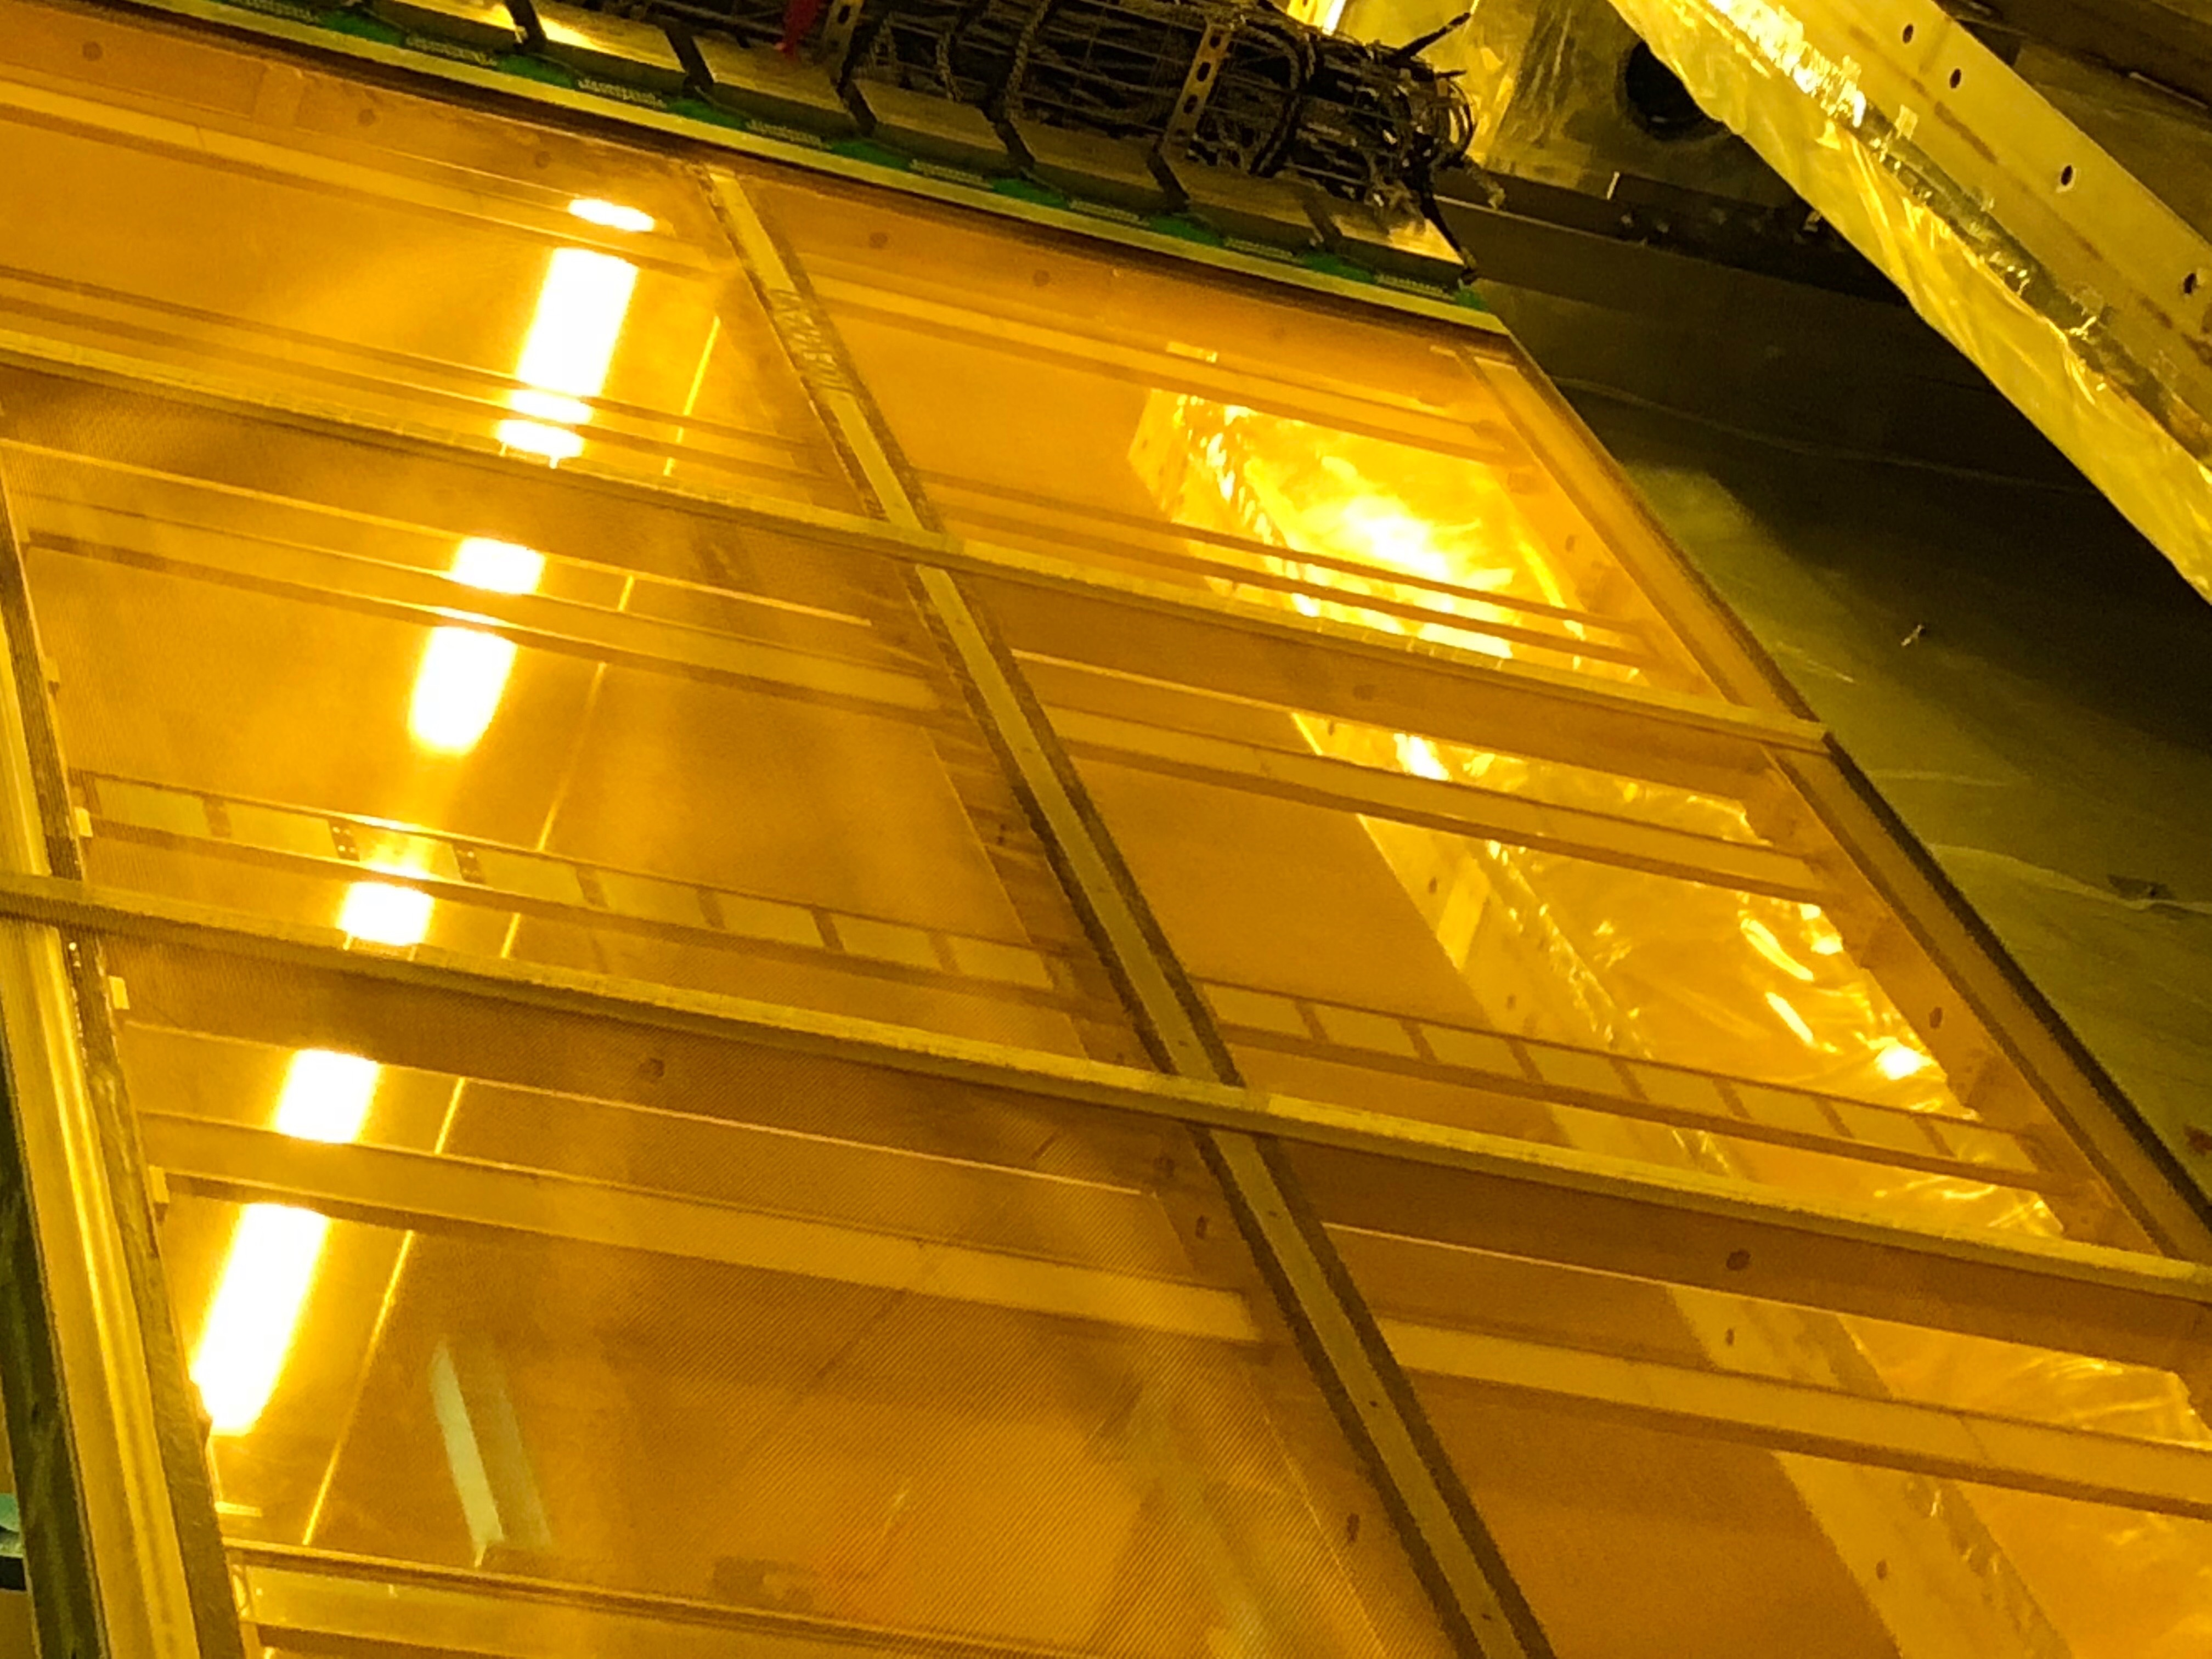
\includegraphics[height=8cm]{pds-arpk-apa3_pd.jpg} 
%\end{dunefigure}

\begin{dunefigure}[Full-scale \dword{sarapu} array installed in \dword{pdsp}.]{fig:arapuca-protodune}
{\dword{sarapu} array installed in \dword{pdsp}.} 
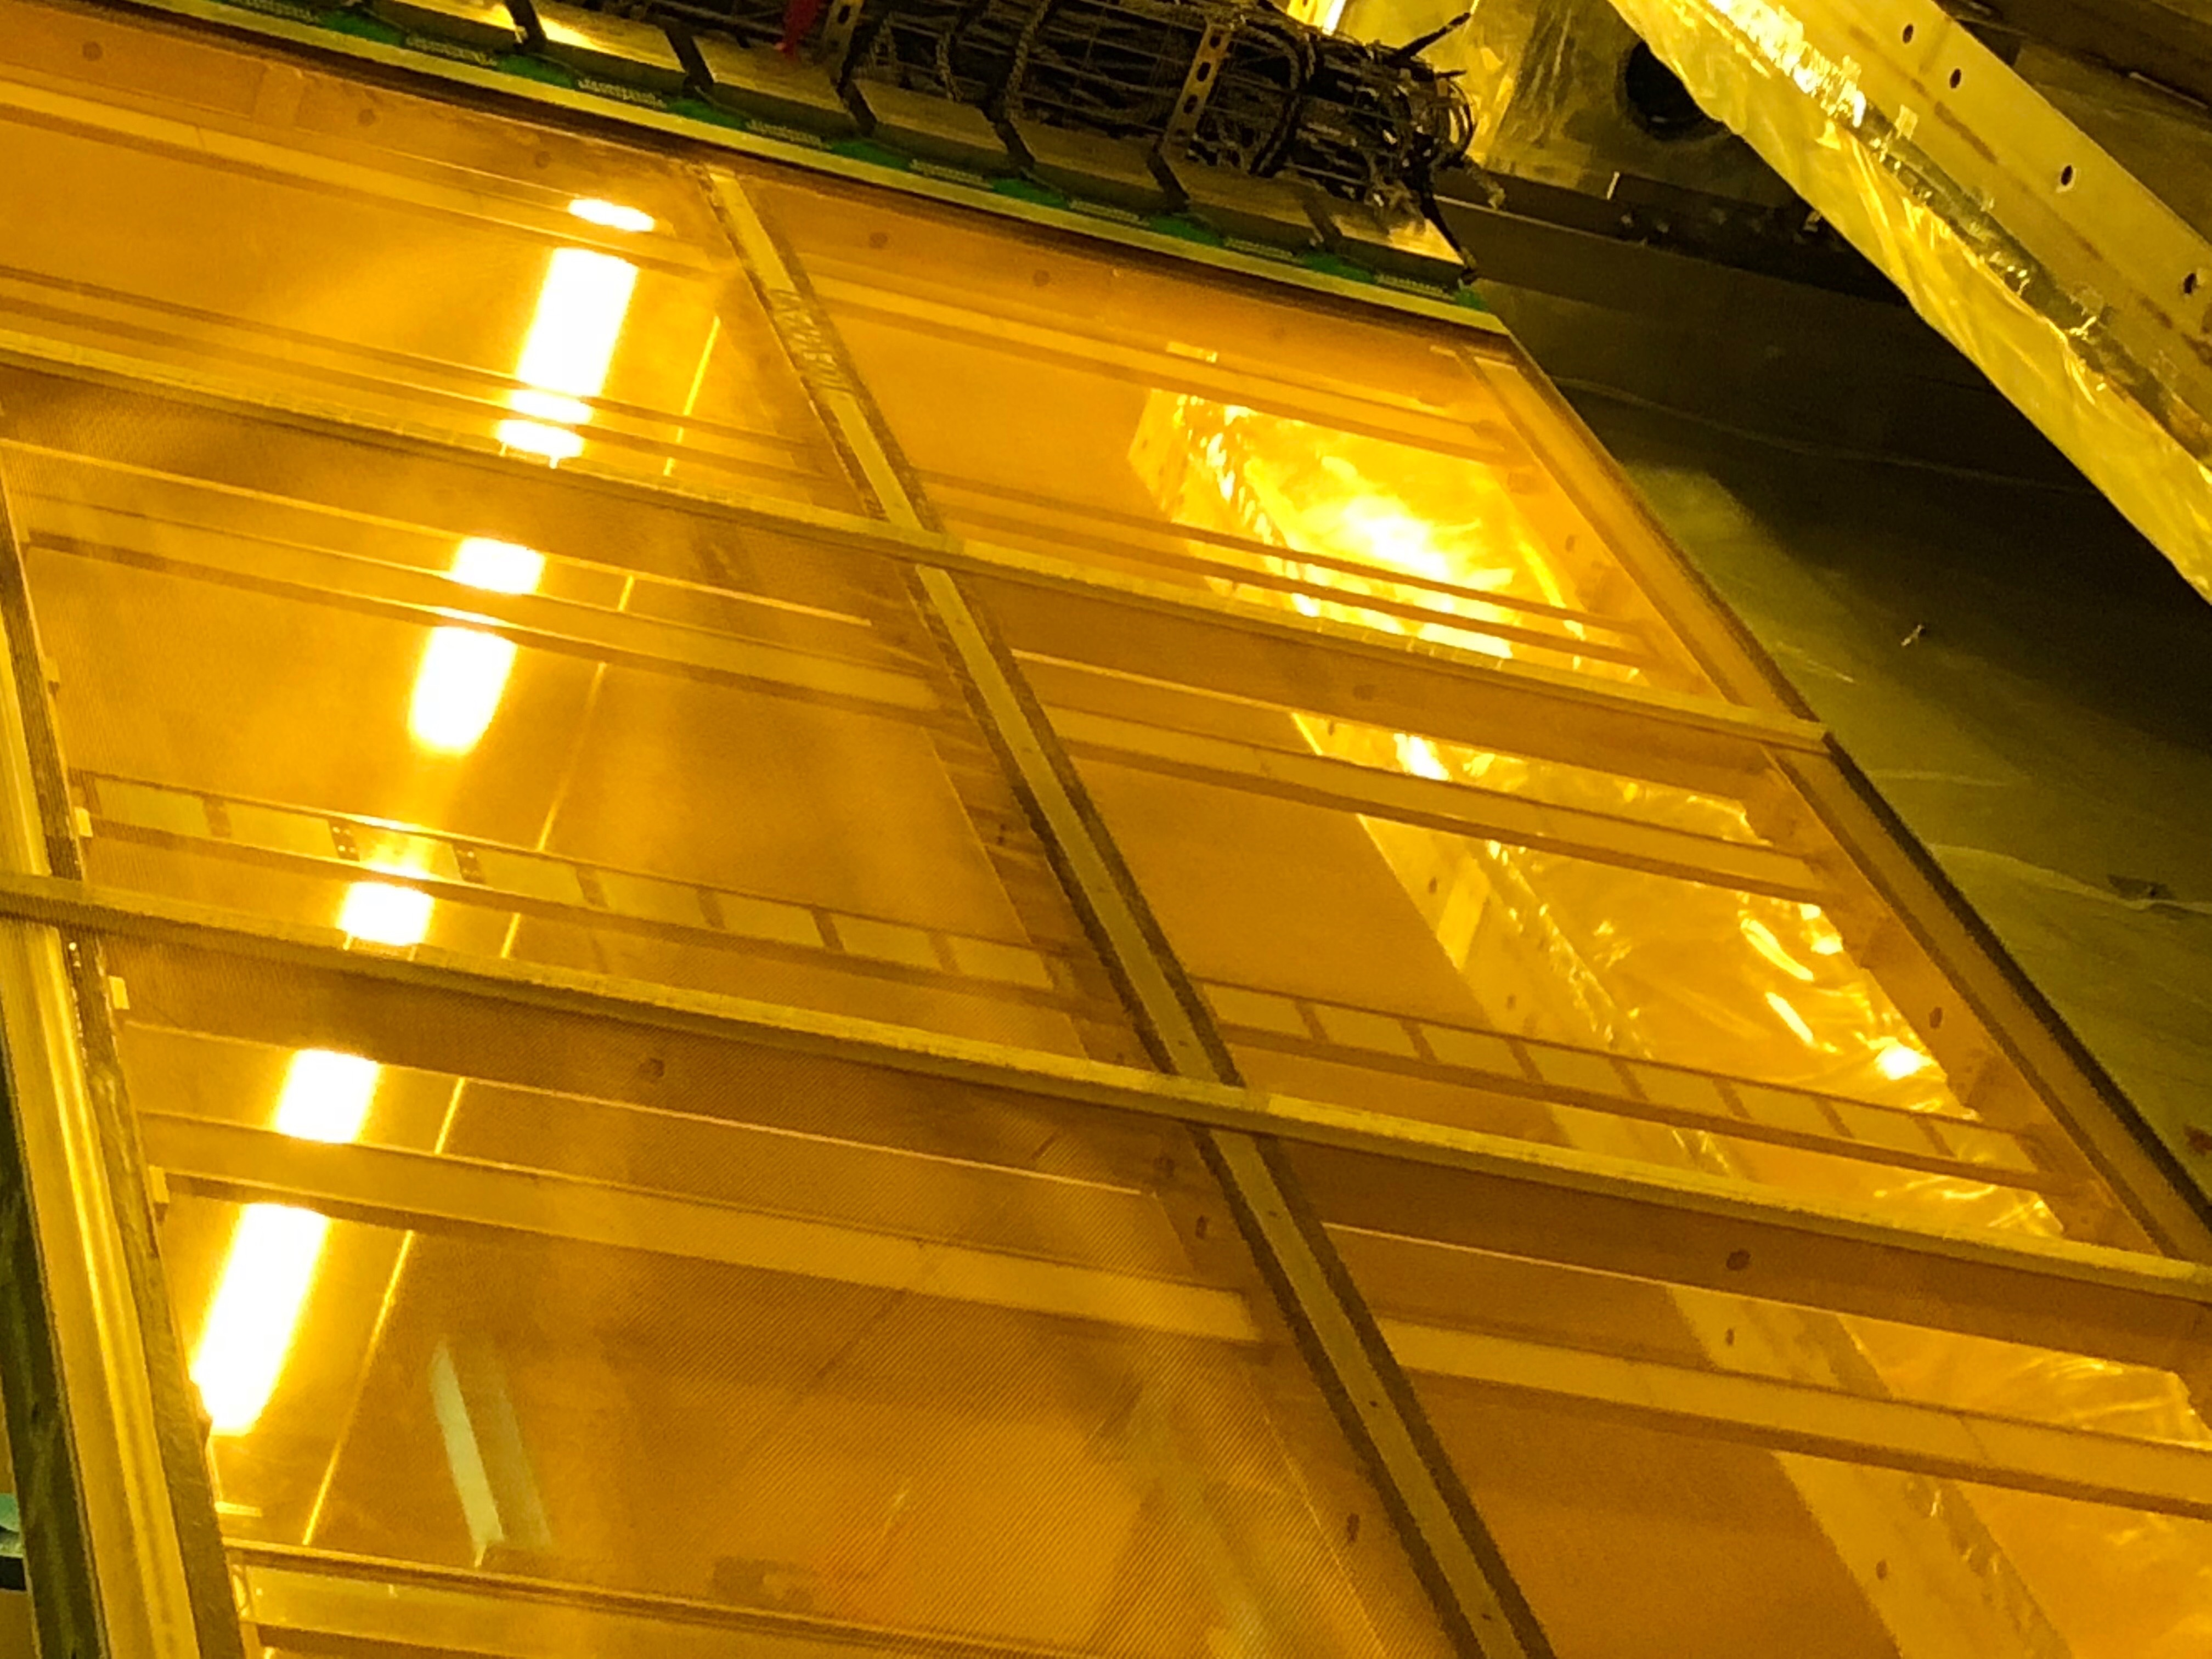
\includegraphics[height=7cm]{pds-arpk-apa3_pd.jpg} 
\end{dunefigure}

%\begin{dunefigure}[\dword{sarapu} array in \dword{pdsp}.]{fig:arapuca_array}
%{ARAPUCA array in \dword{pdsp}dword{pdsp}.} 	
%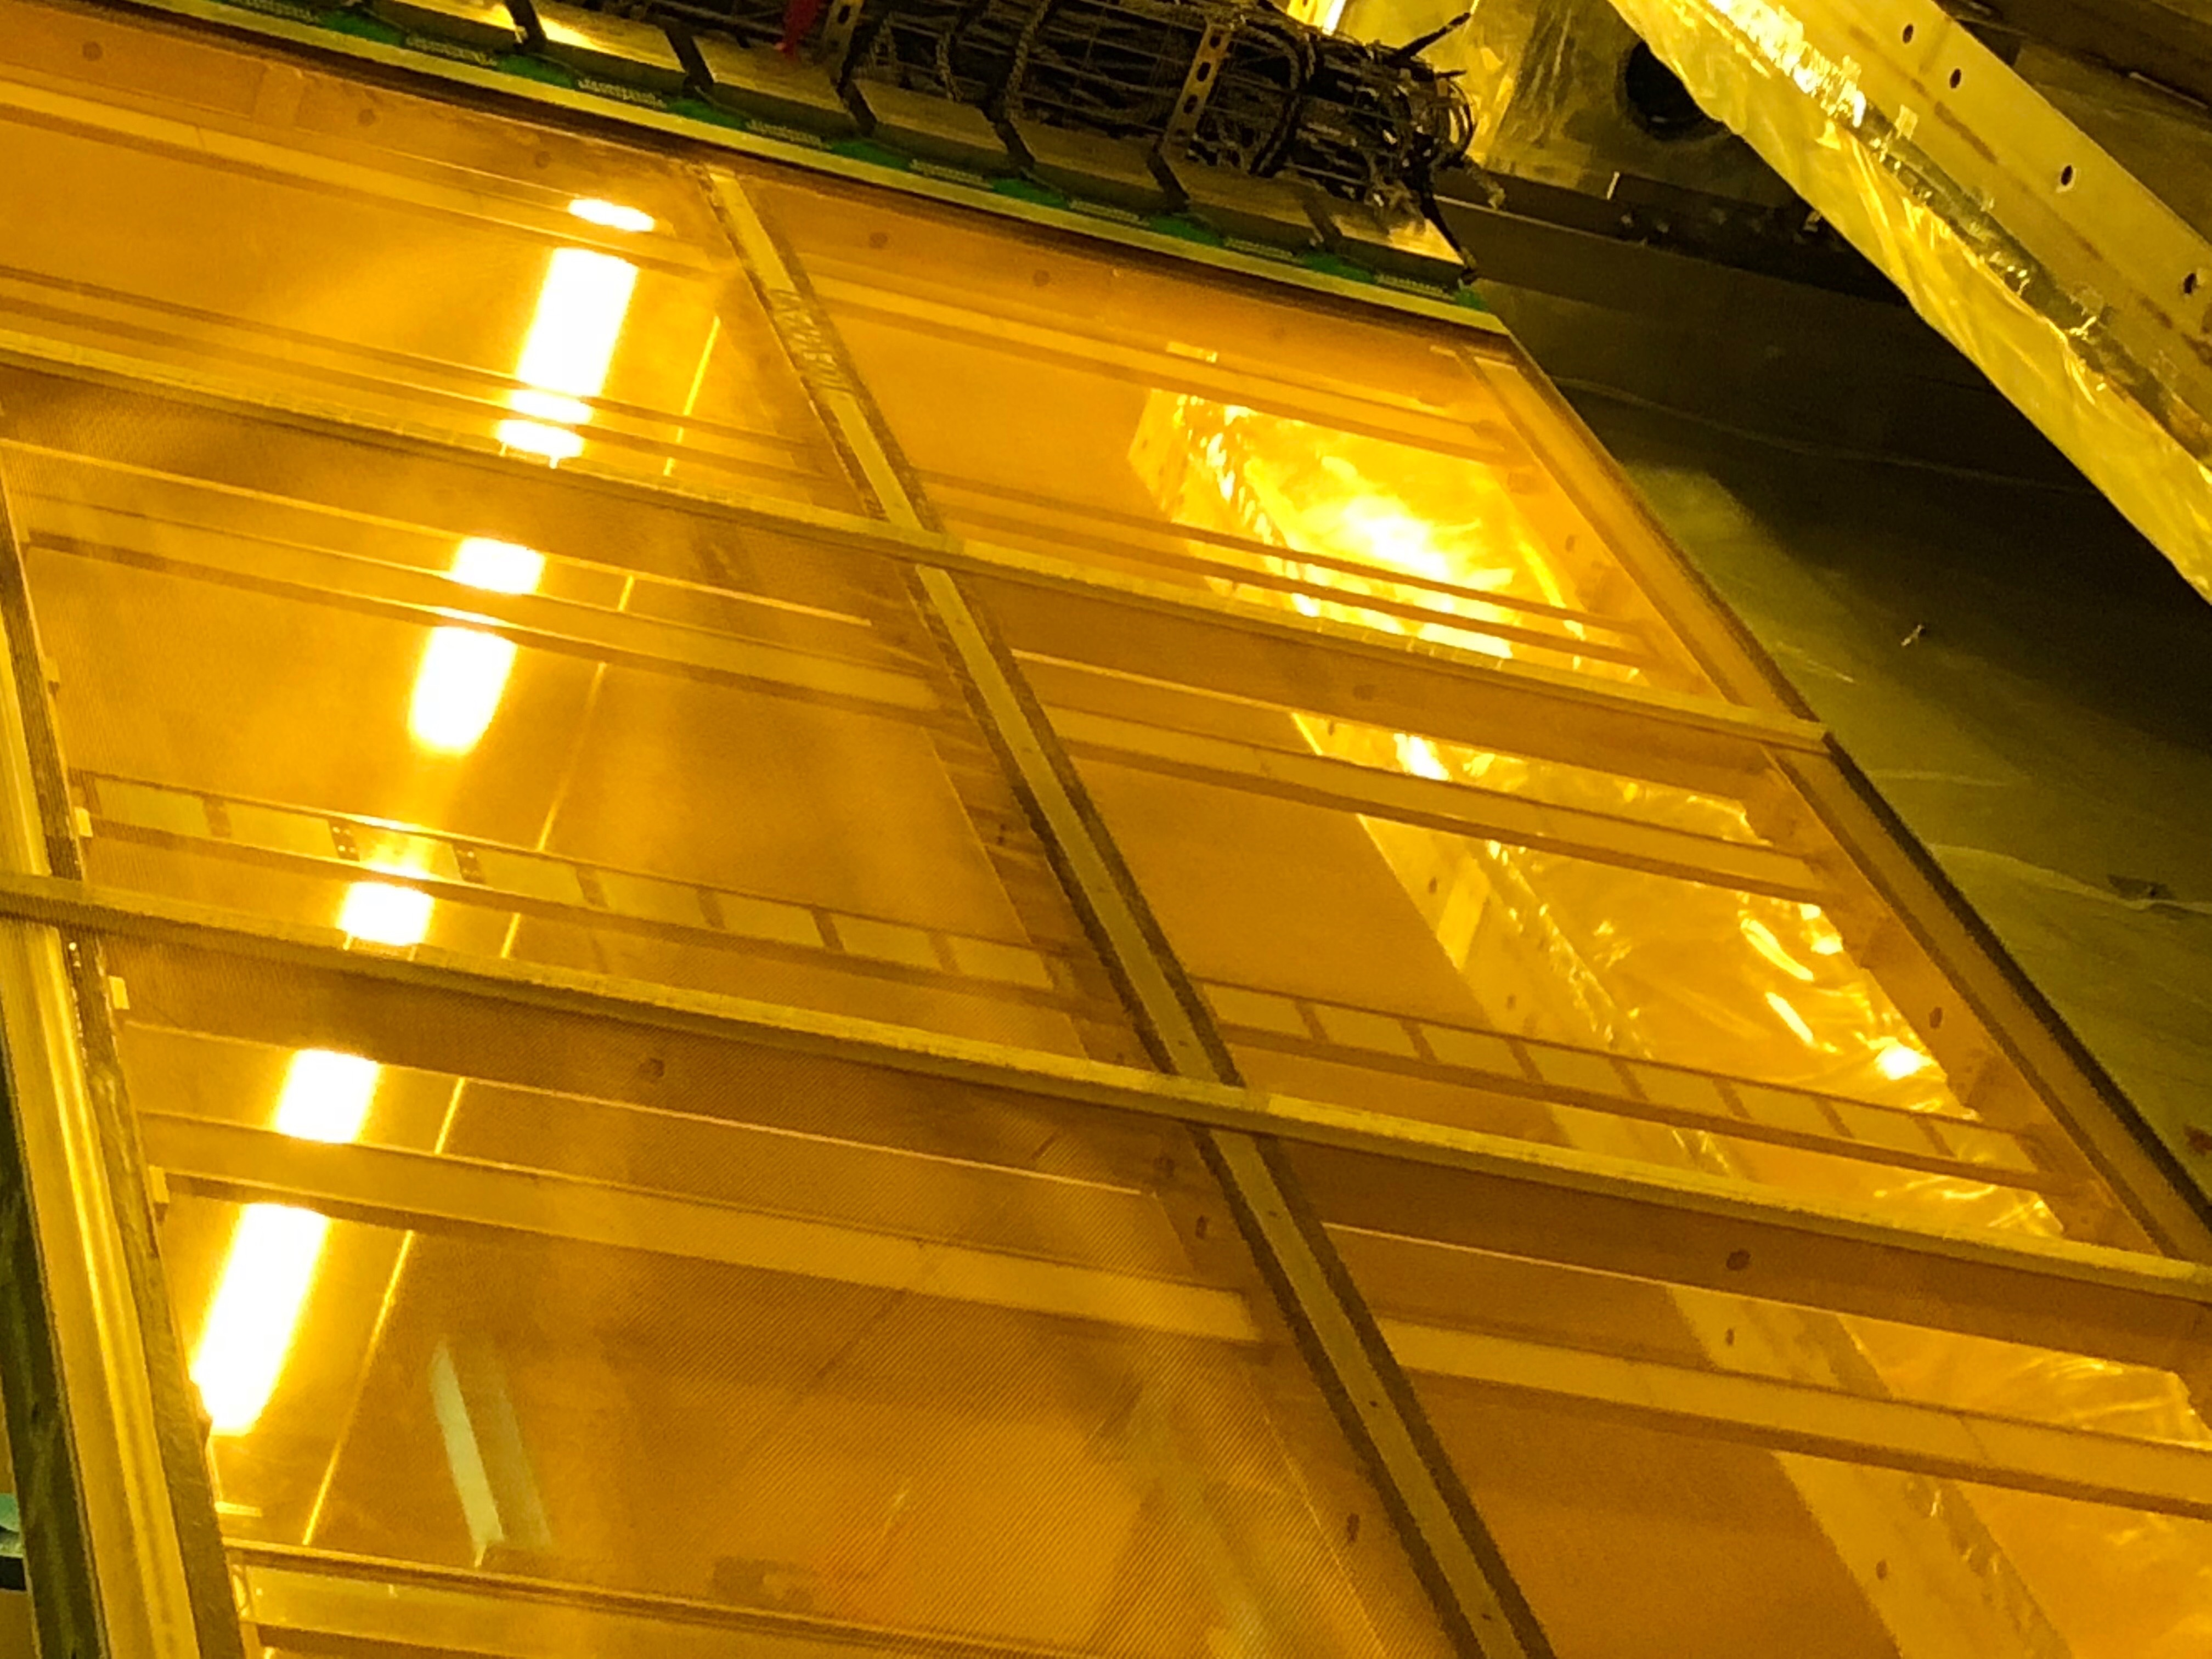
\includegraphics[height=8cm]{pds-arpk-apa3_pd.jpg} 
%\end{dunefigure}

\subsubsection{\dword{pdsp} Electronics}
\label{sec:ssp-protodune-electronics}

%\metainfo{Content: Djurcic}
% SSP references (from Zelimir):
%The current generation of the SSP [1, 2, 3] has been designed and fabricated for photon-detector readout in DUNE prototypes [1, 2, 3, 4]

%1: DUNE Interim Design Report: B.~Abi {\it et al.} [DUNE Collaboration],
%  “The DUNE Far Detector Interim Design Report, Volume 2: Single-Phase Module,”  arXiv:1807.10327 [physics.ins-det].
%2: ProtoDUNE TDR: B.~Abi {\it et al.} [DUNE Collaboration],
%  “The Single-Phase ProtoDUNE Technical Design Report,”  arXiv:1706.07081 [physics.ins-det].
%3: DUNE docdb: https://docs.dunescience.org/cgi-bin/private/ShowDocument?docid=3126
%4: DUNE 35t detector prototype results: D.~L.~Adams {\it et al.} [DUNE Collaboration],
%  “Photon detector system timing performance in the DUNE 35-ton prototype liquid argon time projection chamber,”  JINST {\bf 13}, no. 06, P06022 (2018), arXiv:1803.06379 [physics.ins-det].

The electronics readout of the \dword{pdsp} \dword{pds} was provided by a sophisticated custom-designed system, the \dword{sipm} Signal Processor (\dwords{ssp})~\citedocdb{3126} that was also used extensively for most of the earlier prototyping studies and photosensor testing.
A passive signal summing scheme with three \dwords{sipm} summed together was chosen for the light guides (four \dword{ssp} channels for each bar) and groups of twelve \dwords{sipm} are passively summed for the two ARAPUCA modules (12 \dwords{ssp} channels per module).
The unamplified analog signals from the \dwords{sipm} are transmitted directly to outside the cryostat for processing and digitization. The \dword{ssp} consists of 12 readout channels packaged in 
a self-contained 1U module. The ProtoDUNE \dword{pds} is read out with the total of 288 \dwords{ssp} channels. 
Twenty-four custom \dword{sipm} Signal Processor (\dword{ssp}) units were produced to read out the 58 light guide and two ARAPUCAs photon collector arrays.
%\dword{ssp} at the top of \dword{pdsp} cryostat are shown in Figure~\ref{fig:fig-pds-readout}, right. 
Each channel contains a fully-differential voltage amplifier and a \num{14}-bit, \num{150}-MSPS \dword{adc} that digitizes the \dword{sipm} signal waveforms.

%A dedicated \dword{pd} readout system with a high-performant electronics \dword{fe} was developed for the \dword{pdsp} experiment, as schematically presented in Figure~\ref{fig:fig-pds-readout}, left. 
%For \dword{pdsp}, a passive signal summing scheme with three \dwords{sipm} summed together was chosen for the light guides (4 \dword{ssp} channels for each bar) and groups of twelve \dwords{sipm} are passively summed for the two ARAPUCA modules (12 \dwords{ssp} channels per module).
%The un-amplified analog signals from the \dwords{sipm} are transmitted directly to outside the cryostat for processing and digitization. A custom module, called the \dwords{sipm} Signal Processor (\dword{ssp}), receives the \dwords{sipm} signals outside the cryostat. An \dword{ssp} consists of 12 readout channels packaged in a self-contained 1U module. ProtoDUNE \dword{pds} is red-out with the total of 288 \dwords{ssp} channels. 
%Twenty-four custom \dword{sipm} Signal Processor (\dword{ssp}) units were produced to read out the 58 light guide and 2 ARAPUCAs photon collector arrays.
%\dword{ssp} at the top of \dword{pdsp} cryostat are shown in Figure~\ref{fig:fig-pds-readout}, right. Each channel contains a fully-differential voltage amplifier and a \num{14}-bit, \num{150}-MSPS \dword{adc} that digitizes the \dword{sipm} signal waveforms.
%The \dword{fe} amplifier is configured as fully-differential, and receives the \dwords{sipm} signals into a termination resistor that matches the characteristic impedance of the signal cable. 

%\begin{dunefigure}[\dword{pdsp} \dword{pd} module readout.]
% {fig:fig-pds-readout}
% {Block diagram of the ProtoDUNE \dword{pd} readout module (left figure). Photon-detector \dword{fe} electronics operational 
%at ProtoDUNE (right figure).}
%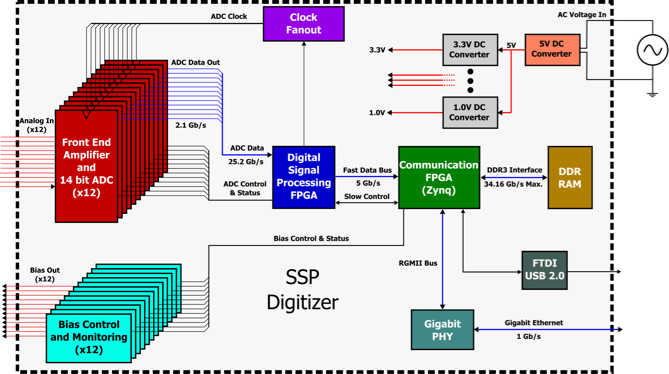
\includegraphics[angle=0,width=8.4cm,height=6cm]{pds-fig-e-3.png}
%\includegraphics[angle=0,width=8.4cm,height=6cm]{protodune_readout.png}
%\end{dunefigure}
%\fixme{LMM 1/13/2018 I'm just going to fix the text below, I left this fixme here thinking it was Zelimir's words and needed fixing.  I'm not seeing anything happening, so I'll just fix it.  -- This was my comment: The triggering here is not really correct for how it was done at protodune.  The module continually digitizes (always) and stores waveforms above threshold in a circular buffer.  On an external trigger, it will send a waveform and header for the time period of the trigger and any stored waveforms or subsequent waveforms above threshold for the configured readout window. For protoDUNE it always send header and waveform, and in all cases if it sends a waveform it will send a header. I'm not sure where the following paragraph comes from? I didn't want to rewrite without knowing where it came from}

%commented here is the original(?) text
%In the standard mode of operation, the module performs waveform capture, using either an external or internal trigger. In the latter case the module self-triggers to capture only waveforms with an amplitude greater than a specified threshold. In \dword{pdsp} the photon readout is configured to read waveforms when triggered by a beam event, or to provide header information when self-triggered by cosmic muons.
%The header portion summarizes pulse amplitude, integrated charge, and time-stamp information of events. The \dword{ssp} for \dword{pdsp} uses \si{Gb} Ethernet 
%communication implemented over an optical interface. The \SI{1}{Gb/s} Ethernet supports full TCP/IP protocol.  Advanced on-board FPGAs are utilized for signal processing (ARTIX-7) and trigger/timing communication (Zynq).

In the standard mode of operation, the module continually digitizes the input signals at \num{150}{MSPS} for each channel.  If a threshold is configured on a channel the \dword{ssp} stores any waveform that meets the trigger condition.  This is called an internally triggered waveform. In an externally triggered waveform the module, the configured waveform window at the time of the external trigger is also stored.  This externally triggered waveform and any internally triggered waveform in the buffer window and any subsequent internally triggered waveforms are transmitted to the DAQ board reader processes for storage. The photon readout is configured to trigger on signals from the central trigger board for a variety of configurable events, beam events, externally triggered cosmic muons from the cosmic ray tagger, periodic triggering, random triggering, or any combination of these.

%The module includes a separate 12-bit high-voltage DAC for each channel to provide bias to each \dword{sipm}. Currently there are two DAC options:  one with a voltage range of 0V to 30V, used with 11 the sensL \dwords{sipm} (17 of the 24 \dword{ssp} units); and the other with a range 0V to 60V for use with the 12 Hamamatsu \dwords{mppc} (seven of the 24 \dword{ssp} units).
%The \dword{ssp}  provides a trigger output signal from internal discriminators in firmware based on programmable coincidence logic, with a standard ST fiber interface to the central trigger board (CTB).
%Input signals are provided to CTB from the beam instrumentation, the \dwords{ssp}, and the beam TOF system. The CTB receives timing information from the \dword{pdsp} timing system and the CTB trigger inputs are distributed to the experiment via the timing system.
%To that end, the \dword{ssp} implements the timing receiver/transmitter endpoint hardware to receive trigger inputs and clock signals from the timing system.

%Other readout components, aside from the \dword{fe} electronics (\dwords{ssp}) included design and implementation of signal feed-through, selection and fabrication.

\subsubsection{\dword{pdsp} \dword{pds} Measurements}
\label{sec:protodune-results}

%\fixme {lmm ProtoDUNE analysis strategy outline.   These enumerated section below will get incorporated into the text as strategy becomes clearer as analysis progresses}
%\fixme{rjw 12/2/18 For now just I think it is better to have just a few words and some of the most relevant results, ideally with a reference to a separate document with all the details :-) (I kept your original text in the file)}

The \dword{pdsp} beam run provides several distinct sets of data for understanding \dword{pds} performance.  
There are data sets with cosmic triggering, randomly, or in coincidence the CRT modules.
There are beam data sets with triggers determined by the beam instrumentation.
There are calibration module data sets, with triggers in coincidence or free running with a configured light pulse. The cosmic ray data and beam data include the TPC and/or CRT information to provide strong constraints on the particle trajectory that will allow us to determine the exposure of each module on an event-by-event basis.  The additional data sets are useful for calibration, and understanding background rates due to other processes.  Beam events also appear to be useful for calibration, as they provide very low level light signals to the modules in the beam-left segment of \dword{pdsp} where the beam particles were not seen directly.

The analysis is ongoing but here we summarize some relevant initial results:
%\fixme{Summarize the key results from ProtoDUNE with emphasis on ARAPUCA and \dword{mppc}.  We should also summarize lightguide  Denver points out, for \dword{xarapu} simulation the results from the IU bars feed into the simulation of the filter/light-trapping from ARAPUCA.  Summarized for beam data with ONLY ARAPUCA  I might be able to add some response of neighbors as well, that might show ARAPUCA is MUCH better}

%\fixme{Include a figure with calibration module pulses seen in different modules, highlighting ARAPUCA and \dword{mppc} channel response.  Maybe just \dword{apa} 5 and 6 with just a few SensL devices, but both an ARAPUCA and many \dword{mppc} bars.  LMM - inlcuding pulser for ARAPUCA is hard.  It looks like the response is much lower than for neighboring bars (wavelength response?)  I don't want that to be misleading.  I may be able to get the beam response of neighboring bars in APA 3 to show a comparison.  It looks like beam is the best bet, and it shows off the difference with the correct wavelength of light for physics.}

\begin{dunefigure}[Raw pulse height detected in ARAPUCA for each readout channel at \num{5}{GeV}.]{fig:arapuca_chanph}
{The black histogram shows the event by event sum of the peak pulse height Peak from each of the \num{12} ARAPUCA channels in the ARAPUCA module during a run at beam particle momentum of \num{5}{GeV}. The color histograms are the distributions of the same events for each of the \num{12} channels.  They have been scaled up by a factor of \num{12} for plotting with the summed distribution. No selection on particle types has been performed.}
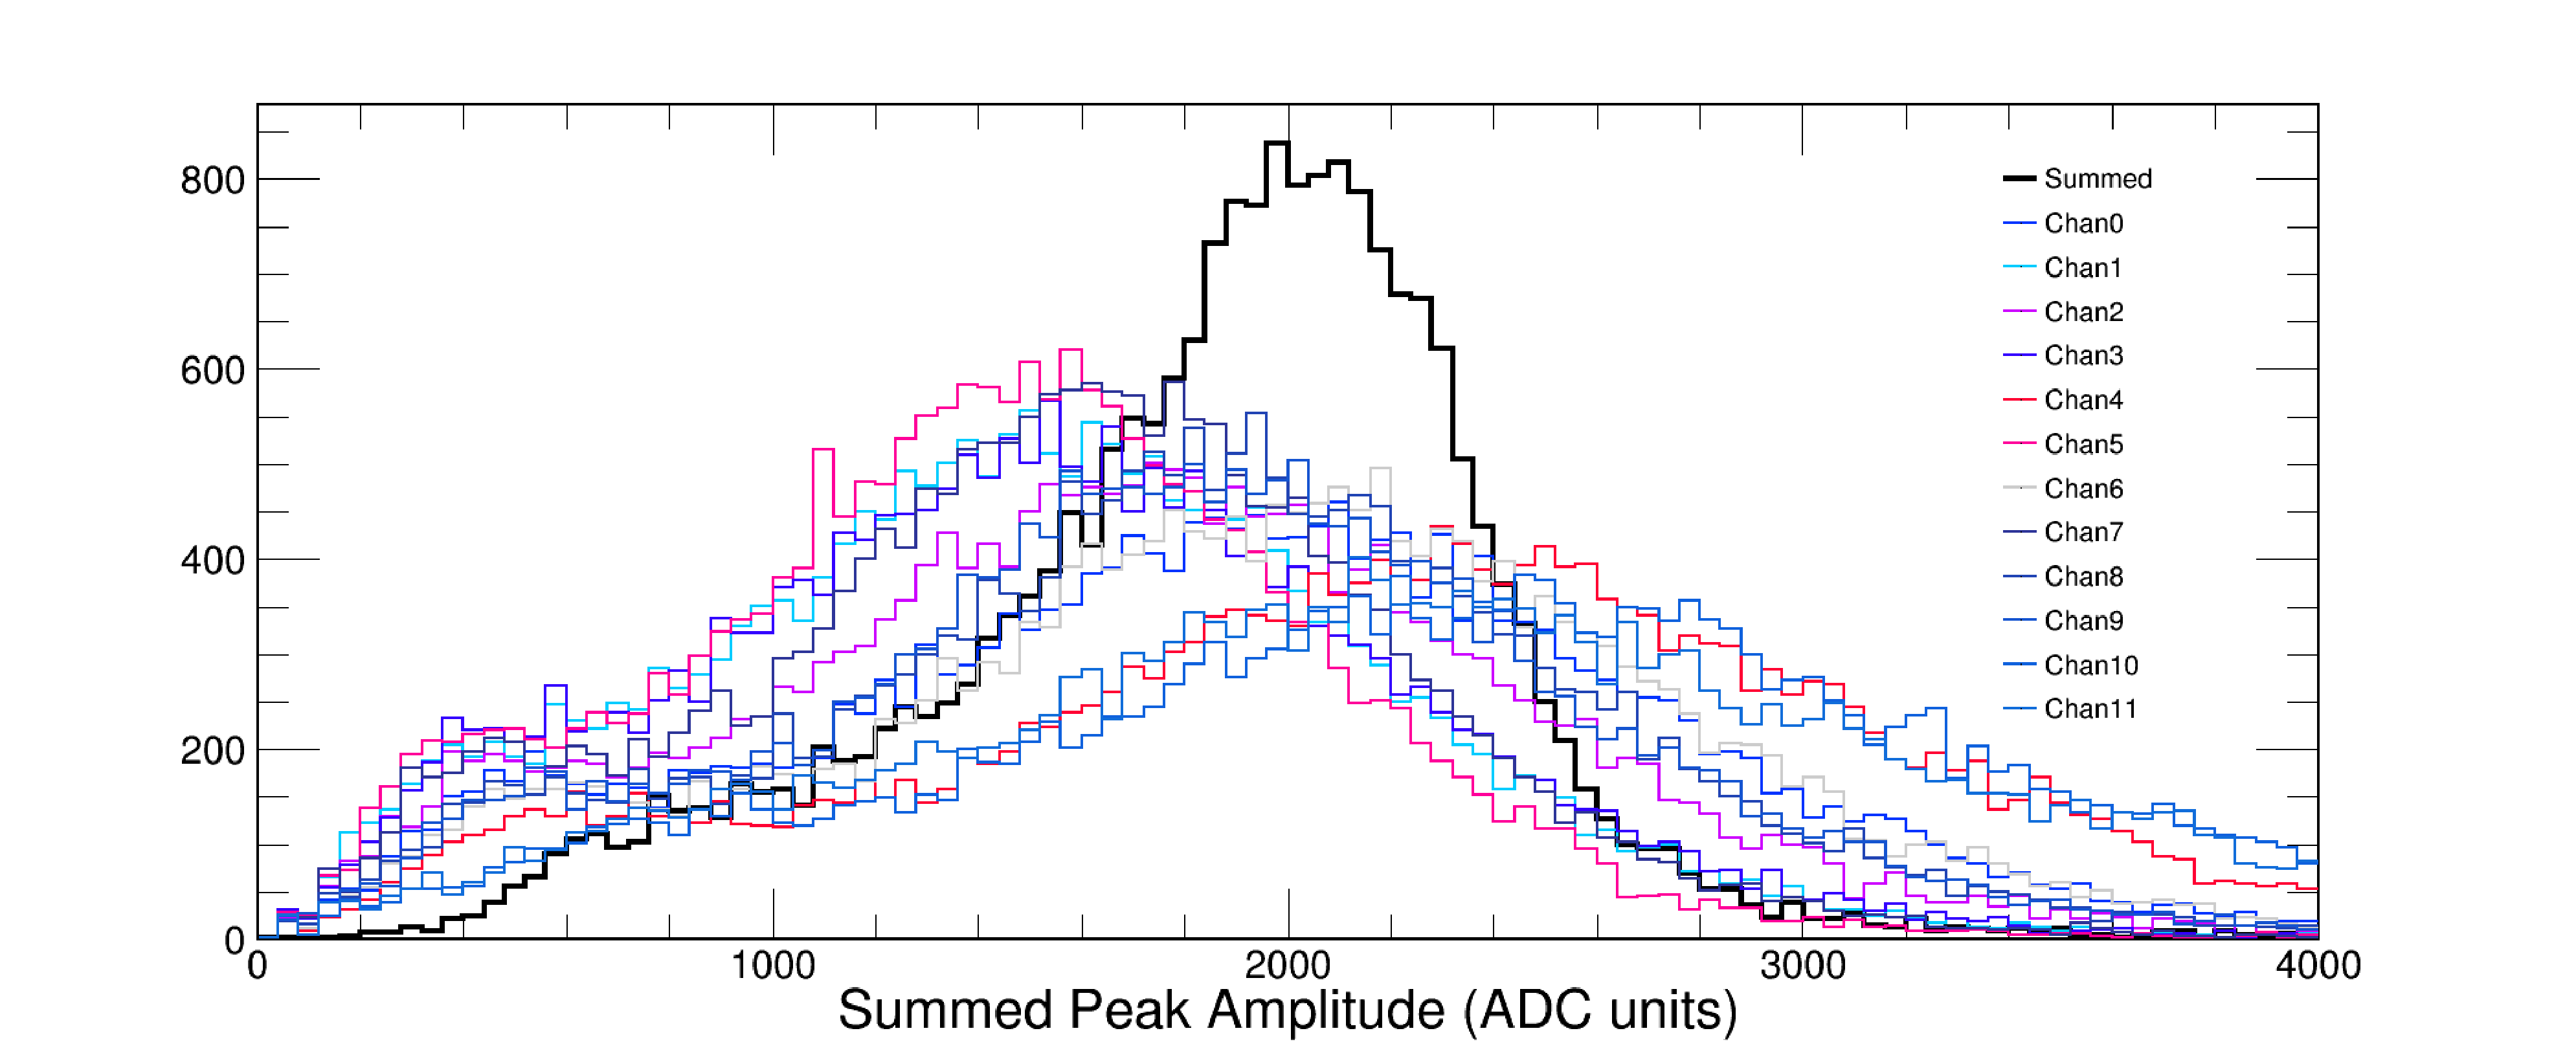
\includegraphics[angle=0,width=\columnwidth]{pds-Arapuca-PHchan.pdf}
\end{dunefigure}

\begin{dunefigure}[Raw pulse height detected in ARAPUCA for different energies.]{fig:arapuca_beamph}
{Peak pulse height in ADC counts summed from all 12 channels in an ARAPUCA module exposed to the beam at beam momenta of \num{1}, \num{3}, \num{5}, and \num{7}{GeV}. No selection on particle types has been performed.}
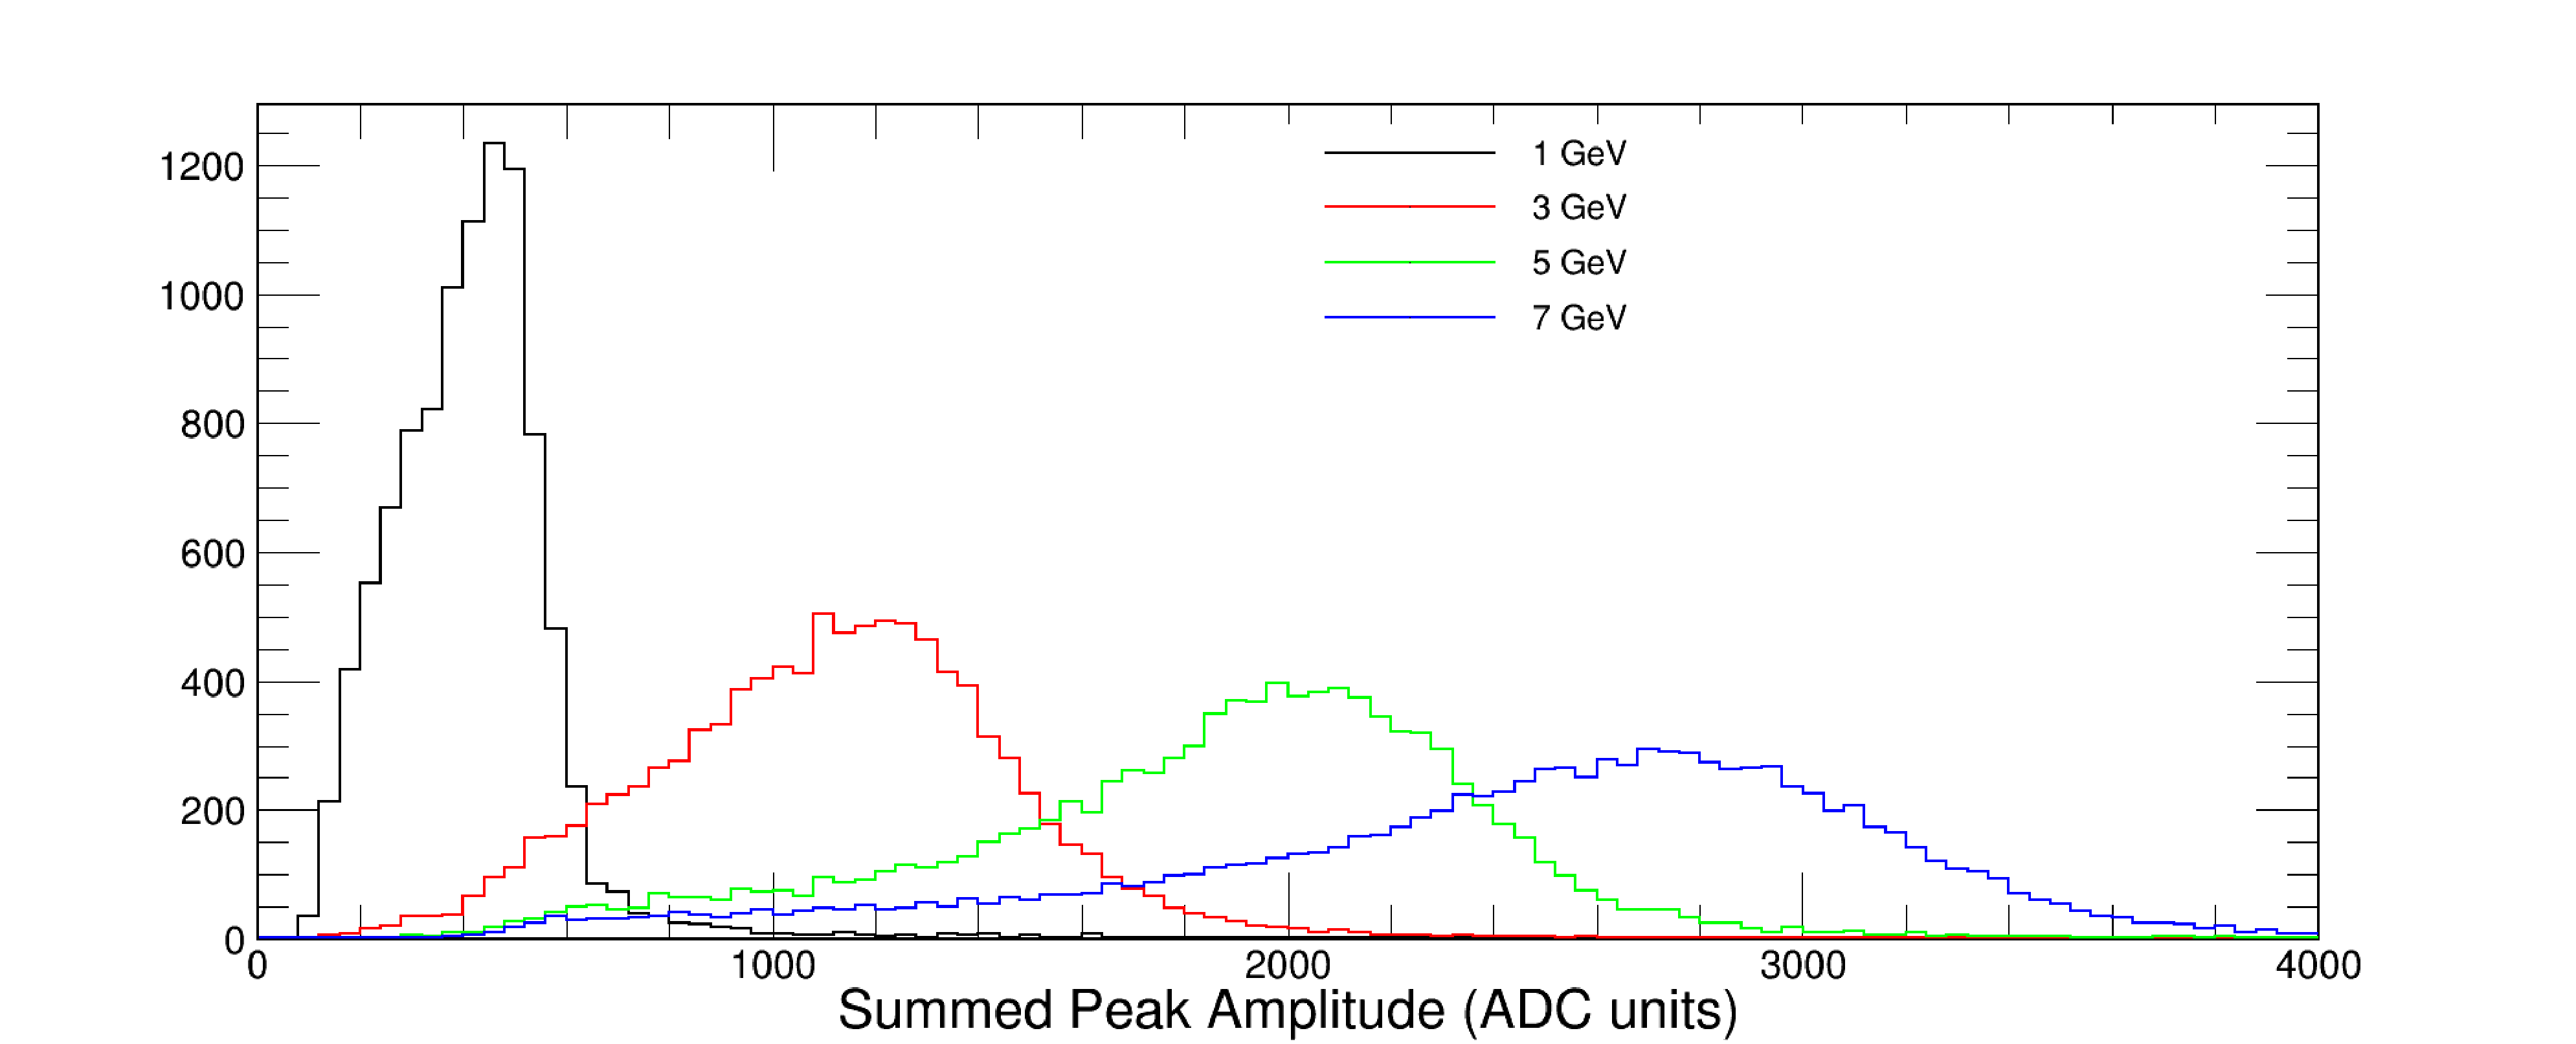
\includegraphics[angle=0,width=\columnwidth]{pds-Arapuca-summedBeamPH.pdf}
\end{dunefigure}

The detector has collected data under many different conditions, including a range of energies from the EHN1 beam line.  The black histogram in Figure \ref{fig:arapuca_beamph} shows the summed response of all \dword{sarapu} cells in the module to beam triggered events in \dword{pdsp}.  The pulse height distribution, scaled up \num{12} times for display, from each of the \num{12} channels are shown by the colored histograms.  Differences between the individual channels and the summed histogram are due to geometric effects, light collection, gain, and other variation.  A detailed analysis of each event will help understand and predict the response of photon detectors in a large liquid Argon detector.
Initial work has determined the single avalanche response for each of the \num{256} readout channels in \dword{pdsp}. The correction for this response variation would be less than 10\% and has not been applied to the data shown.
%Not sure if we should show the pe peaks, we don't understand why some are much better than others, so it might be misleading.
%This is part of the information needed to calibrate the response of each channel. In order to fully determine the response the crosstalk must also be measured.  

Figure \ref{fig:arapuca_beamph} shows the pulse height distribution for 4 different beam momenta of \num{1},\num{3}, and \num{7}{GeV}, in addition to the \num{5}{GeV} data shown in figure \ref{fig:arapuca_beamph} .  As before, the pulse height for each event in the histogram is the sum of the peak amplitude from each of the \num{12} \dword{sarapu} channels in the slot.  All beam events are included. The distribution of particle types will vary with energy, so the distributions are not expected to be identical.  They do show the expected increase with energy.  A full analysis is underway that will take into account the full details recorded for each of the events.  
 
%\begin{itemize}
%\item Random Cosmic events - broad distribution mostly vertical
%\item CRT Cosmic events - broad x-y dist mostly horizontal
%\item Beam events - well localized, controlled energy
%\end{itemize}

%There are 3 sets of data with distinct features, in all cases the TPC and/or CRT will provide strong constraint on the detailed particle trajectory for measuring exposure of each module on an event by event basis.
%\begin{itemize}
%\item Random Cosmic events - broad distribution mostly vertical
%\item CRT Cosmic events - broad x-y dist mostly horizontal
%\item Beam events - well localized, controlled energy
%\end{itemize}
%Utilize these sources for their unique features.  Initially one can simply select similar events for all modules.  For example, only select tracks that are within 50cm of the cathode, and vertical.  This will strongly limit any dependence on the modeling of light propagation, as the distance will be well controlled.  In this case, relative comparisons could be performed with minimal dependence on any correction factors, geometric or propagation dependent.

%\begin{enumerate}
%\item Calibrate each type of module/sensor (depends on sensor/ganging multiple)  Calibration module may play a large role here, but uncertain at the moment, most have single PE peaks already for calibration
%\item Look at Cosmic pulse height or integral  distributions (can be in parallel)
%\subitem See if stable for given module run to run, and within runs (beginning and end, ...)
%\subitem If yes, see how much modules of same type/readout vary by location 1vs3vs5vs7vs9, and 2vs4vs6vs8vs10... where technology is the same
%\subitem if not well defined, limit trajectories until it is.
%\subitem    if slow enough change, use to predict light in each module (something like distribution peak or mean or 1/2 maximum vs. position) 
%\subitem compare based on module types.  (only one or 2 measurements for ARAPUCA, so they would just be relative comparison of another type of module at that location.
%\item  Using tracking from CRT and/or TPC reconstruct event by event light distribution, and use to determine model parameters, photons/cm, Rayleigh scattering length, ...  (will take a fair amount of data, I suspect)
%\subitem using above, should determine pe/MeV (or pe/cm) for each type of module and at each location in the detector.
%\subitem Beam events can also be used to calculate absolute parameters, but only after determining propagation parameters of \lar 
%\end{enumerate}


\subsection{Single Cell \dword{xarapu} Measurements}
\label{sec:xarapuca-unicamp}
%\metainfo{Content: Segreto/Machado}
%\fixme{First draft by Warner.  Should be edited and corrected by Segreto/Machado. Second draft edited by Segreto.}

The first tests of an \dword{xarapu} cell were made at Unicamp, Brazil at the end of November 2018. 
The structure of the cell used for this test was designed to allow for operation as an \dword{sarapu} or an \dword{xarapu}, with single- or double-sided readout in both configurations.  This flexibility will allow relative and absolute measurements of performance in the same cryostat and so provide a crucial step to validating the baseline design selection.

Building on the experience with the \dword{pdsp} prototypes, the frames for the test cell were fabricated from FR-4 G-10 in a configuration very similar to that planned for the \dword{fd}, but with some small modifications necessitated by the requirements for holding a single-window. The overall dimensions of the cell are \SI{123}{cm}$\times$\SI{100}{cm}$\times$\SI{15.6}{cm}. Figure~\ref{fig:xarapuca-cell} shows an exploded design drawing and the completed cell. 

\begin{dunefigure}[\dword{xarapu} test cell.]{fig:xarapuca-cell}
{\dword{xarapu} test cell:  Assembled cell (left); exploded model(right).  Note that exploded components can be duplicated on the back side (not shown) for double-sided test cell} 
	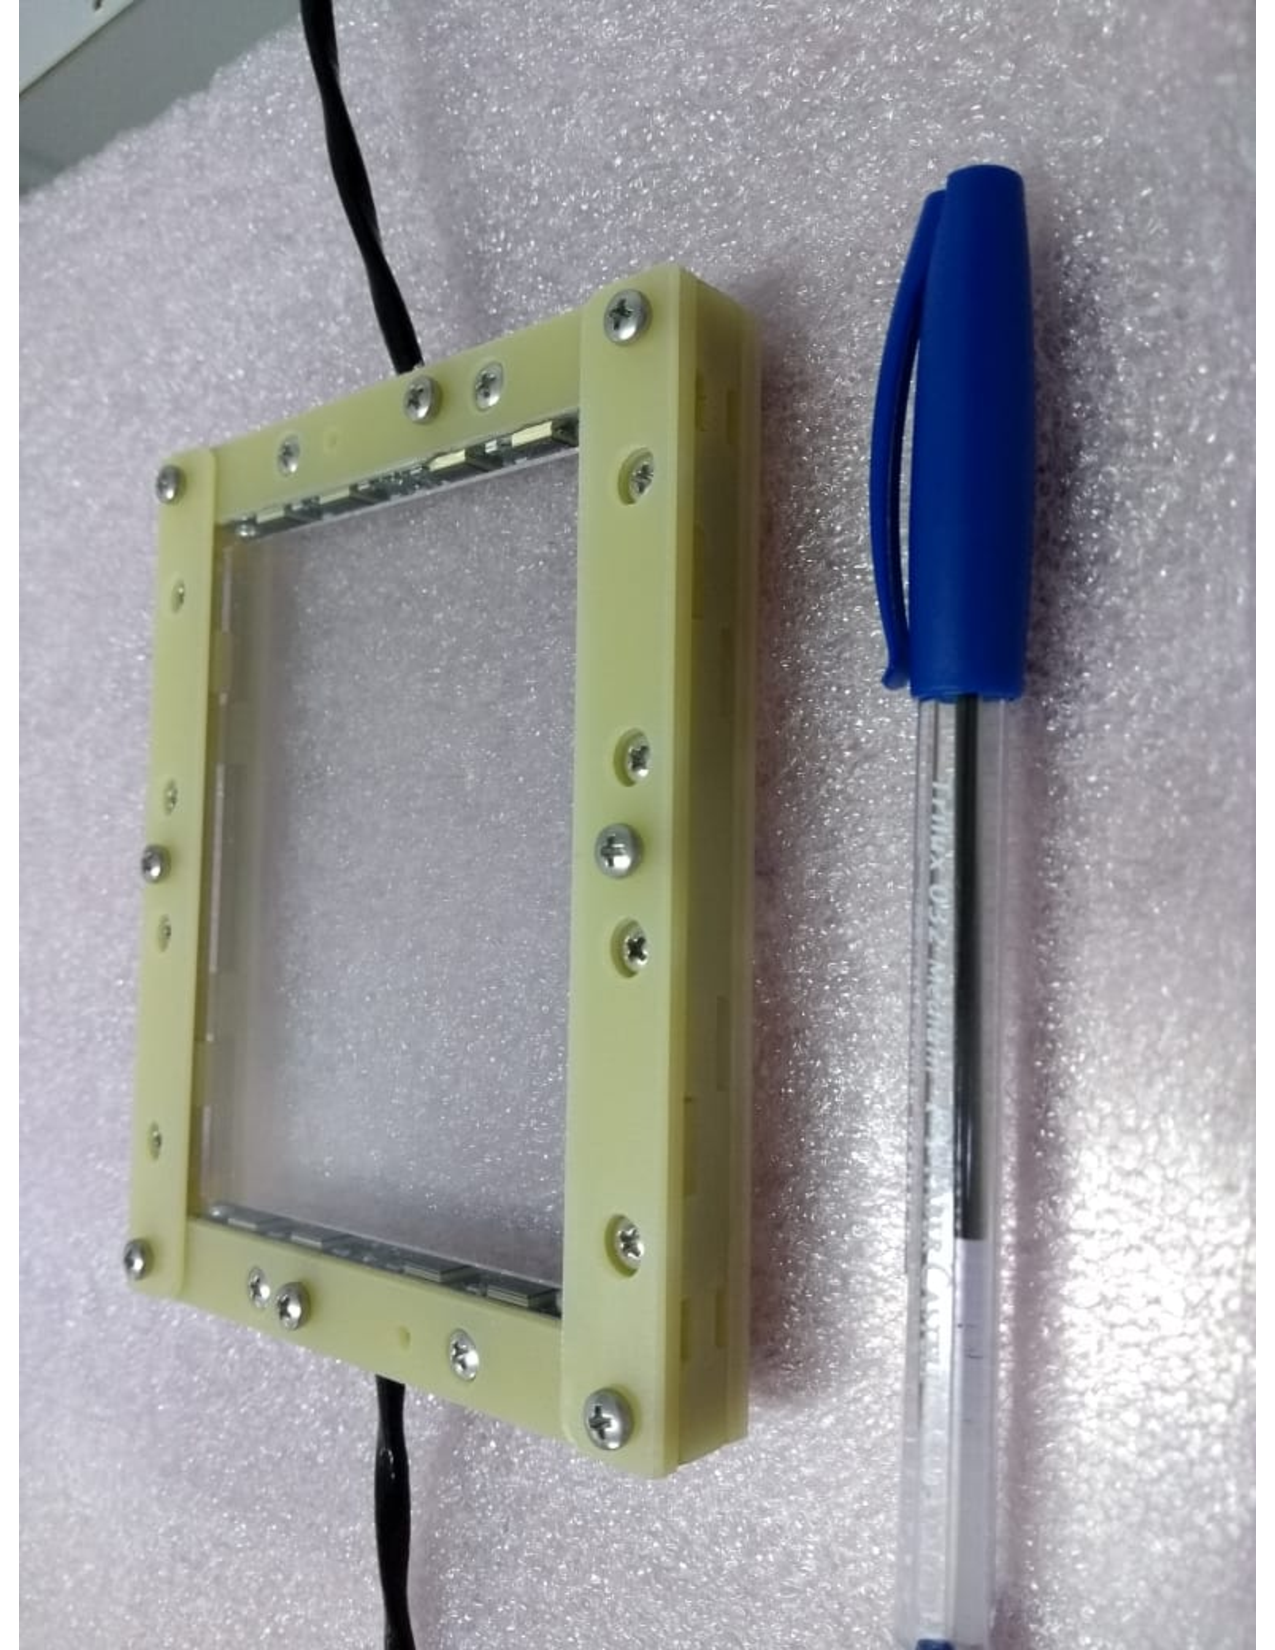
\includegraphics[angle=270, origin=c, width=7cm]{pds-x-arapuca-test-cell-image-2}
	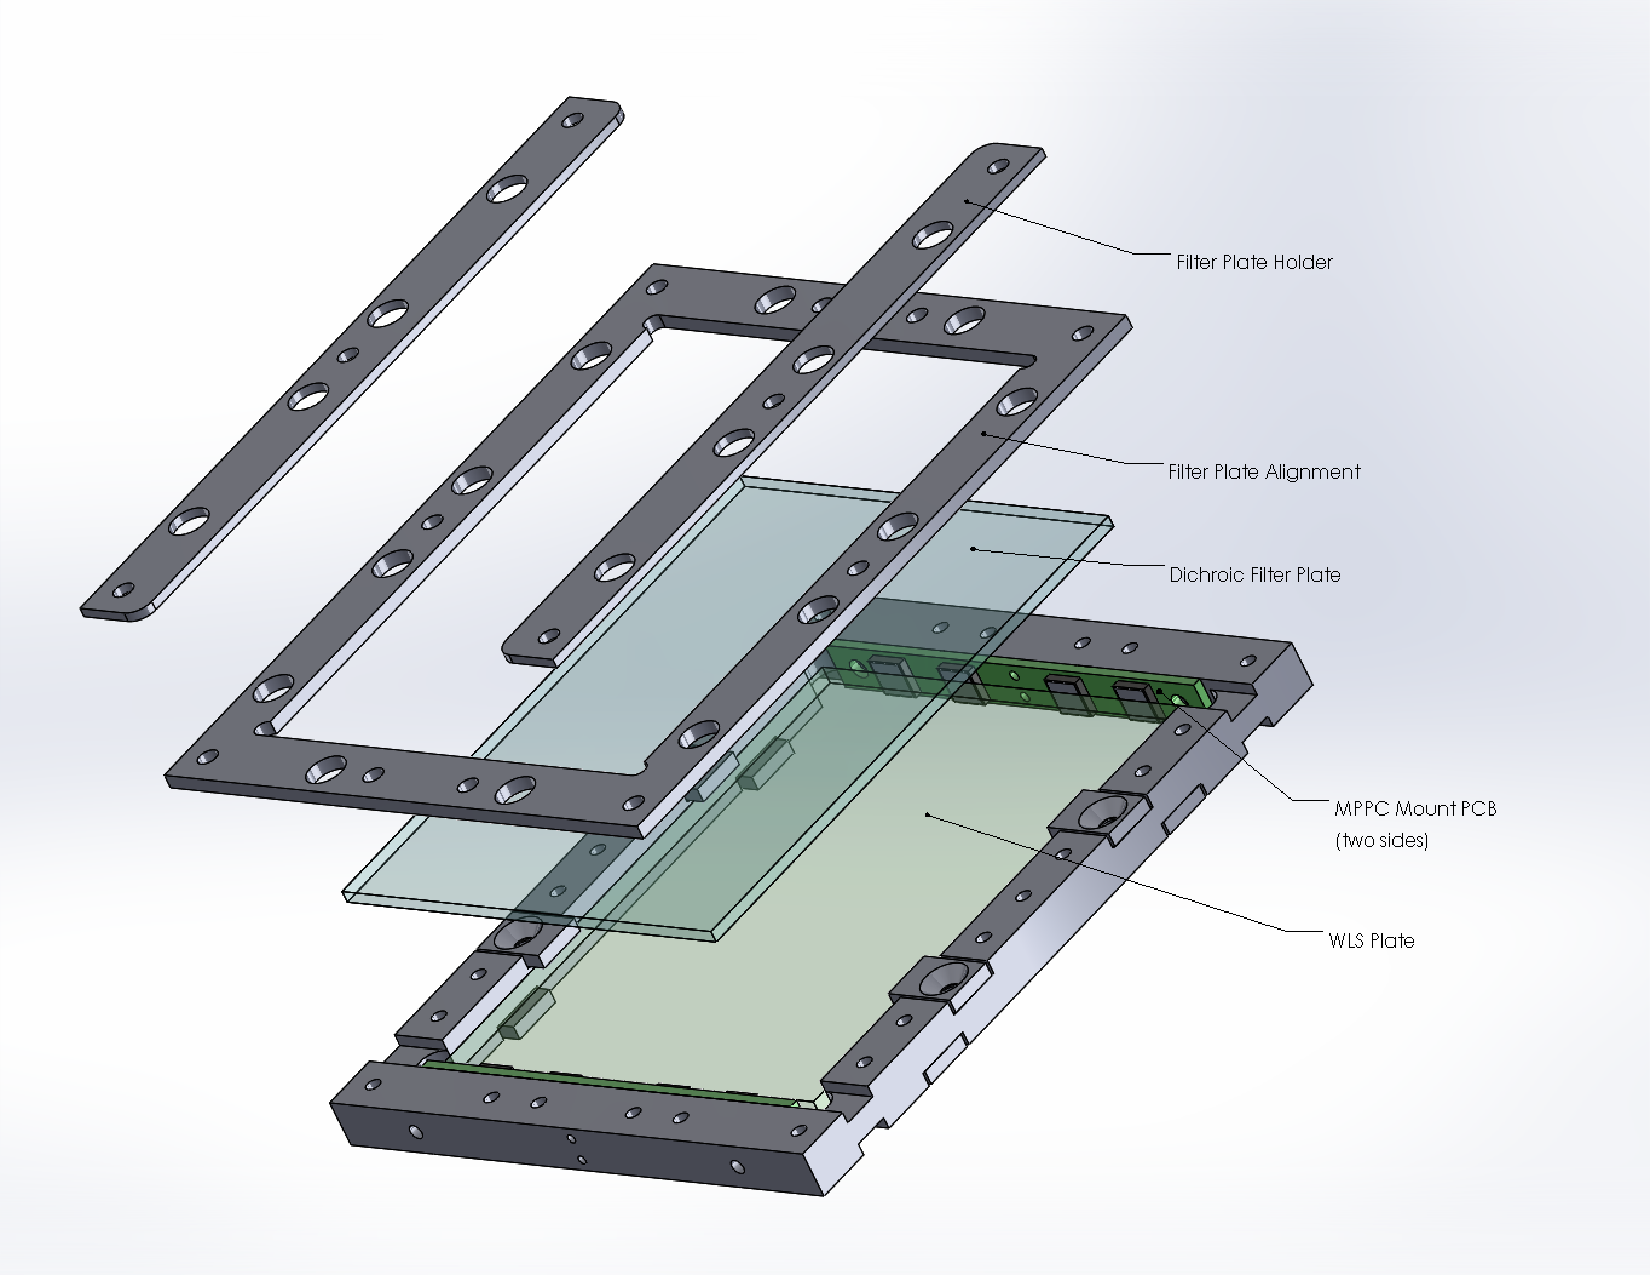
\includegraphics[height=6cm]{pds-unicamp-single-cell-arapuca-exploded}
\end{dunefigure}

The dichroic windows for the prototype are the same size as one of the six windows in a \dword{fd}-design ARAPUCA supercell: \SI{10.0}{cm}$\times$\SI{7.8}{cm}. The filter plate was coated with pTP by vacuum evaporation (film thickness $\sim$ \SI{400}{${\mu}$g/cm$^2$})  using an in-house deposition system at Unicamp. The adhesion was tested by soaking the coated filter in liquid nitrogen few times. No detachment of the evaporated film was observed

The wavelength shifting plate in the \dword{xarapu} configuration is made from Eljen EJ-286 blue WLS plate, with dimensions \SI{9.3}{cm}$\times$\SI{7.8}{cm}$\times$\SI{0.3}{cm}.  The side walls of the test cell are lined with Vikuiti reflector, with cutouts at the positions of the photosensors.

\begin{dunefigure}[Coated dichroic filters and vacuum coating system.]{fig:xarapuca-plates}
{Coated dichroic filter plates (left) and Unicamp thin film coating facility (right).} 
	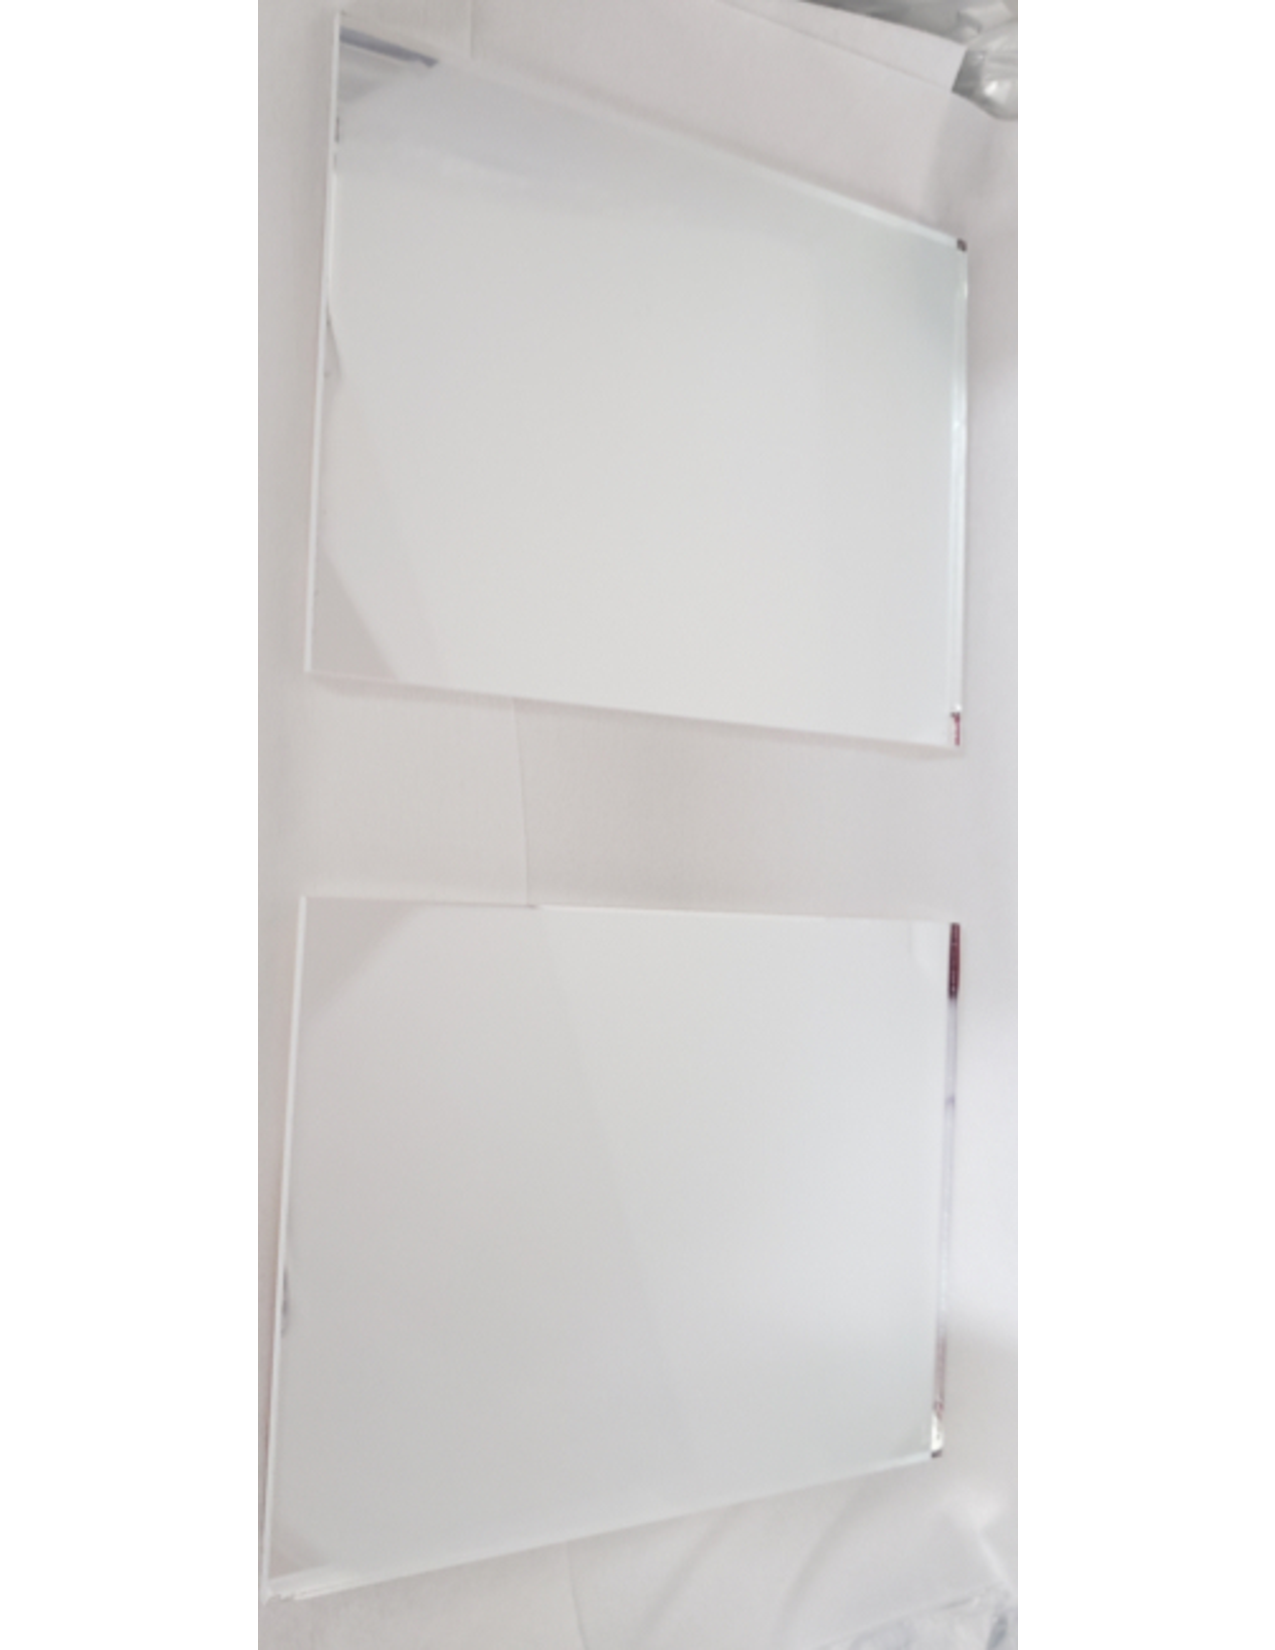
\includegraphics[angle=90, height=6cm]{pds-coated-filter-plates-unicamp}\quad
	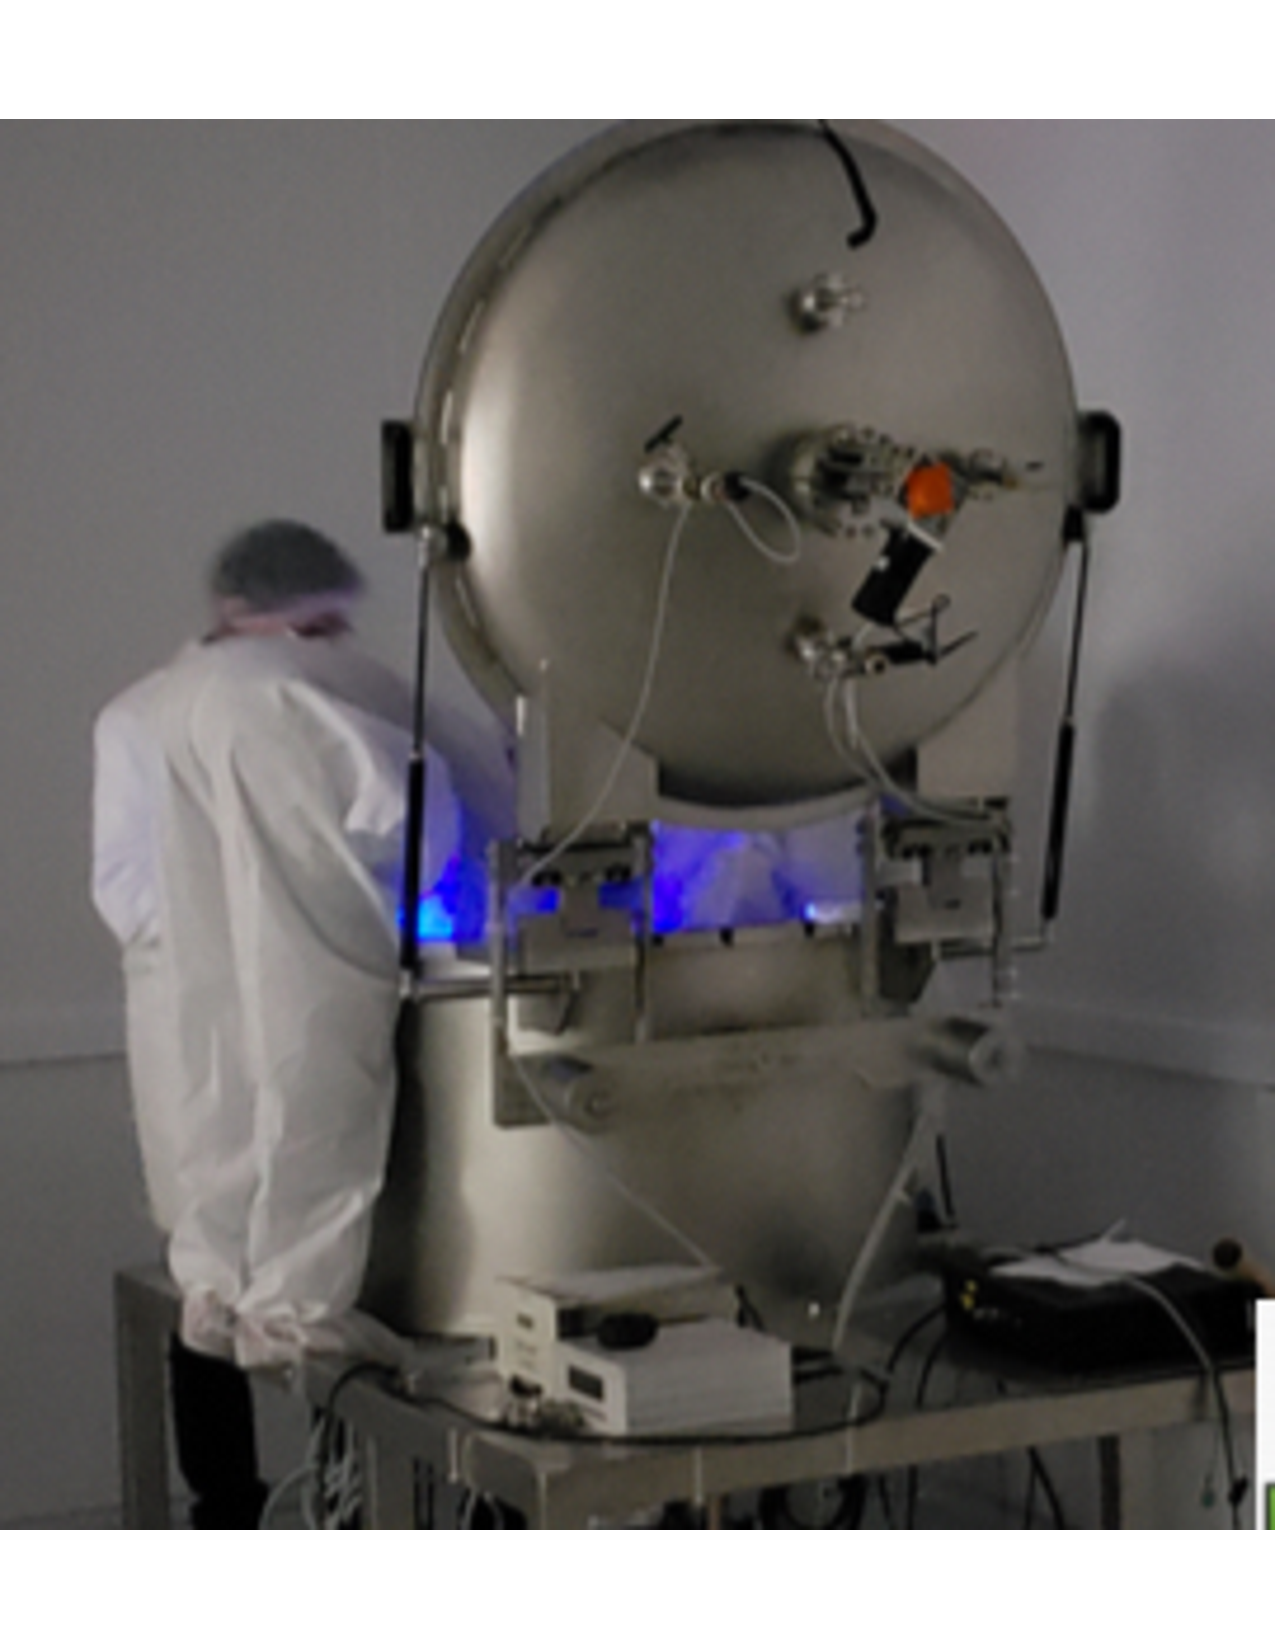
\includegraphics[height=7cm]{pds-unicamp-coating-machine}
\end{dunefigure}

The photosensors in the test cell are of the current baseline design:  \SI{0.6}{cm}$\times$\SI{0.6}{cm} Hamamatsu S13360-6050VE \dwords{mppc}.  The photosensors are arranged in the same configuration as in the baseline design, with four \dwords{mppc} (passively ganged) mounted to two sides of the test cell, with positioning relative to the WLS plates and dichroic filters identical to the baseline design.  In a departure from the baseline design, the two passively ganged groups of 4 \dwords{mppc} are read out separately--no active ganging circuit is implemented for these tests. 

The test cell is installed at the bottom of a  vacuum-tight  stainless-steel cylinder (height $\sim$ \SI{30}{cm)} closed by two CF160 flanges and it is exposed to an alpha source placed at \SI{3}{cm} from the center of the dichroic window. Figure~\ref{fig:xarapu-teststand} shows photos of the test cryostat and the test cell in the support structure; the alpha source holder is visible through the windows.

\begin{dunefigure}[\dword{xarapu} test stand.]{fig:xarapu-teststand}
{Test cryostat at Unicamp (left) and \dword{xarapu} test cell mounting structure (right).  Note the alpha test source in holder.} 
	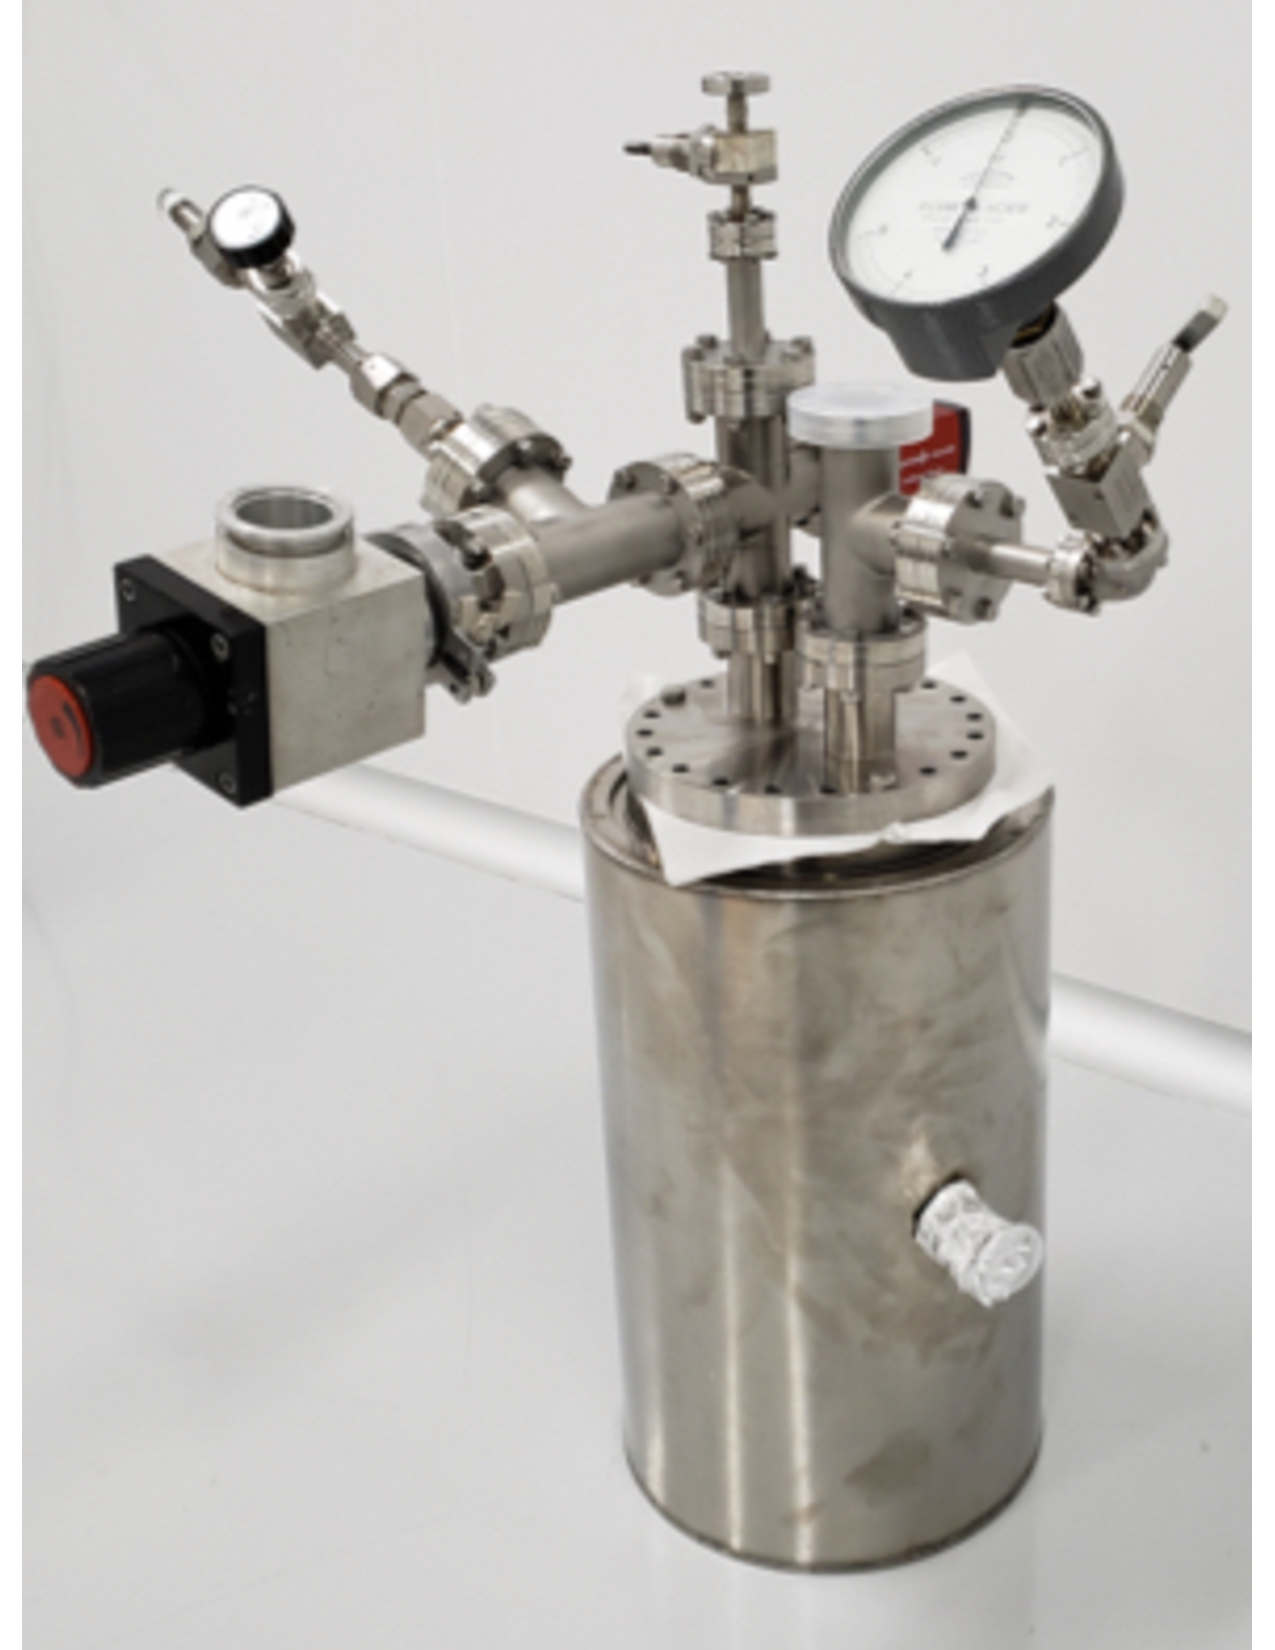
\includegraphics[height=6cm]{pds-unicamp-test-cryostat} \quad
	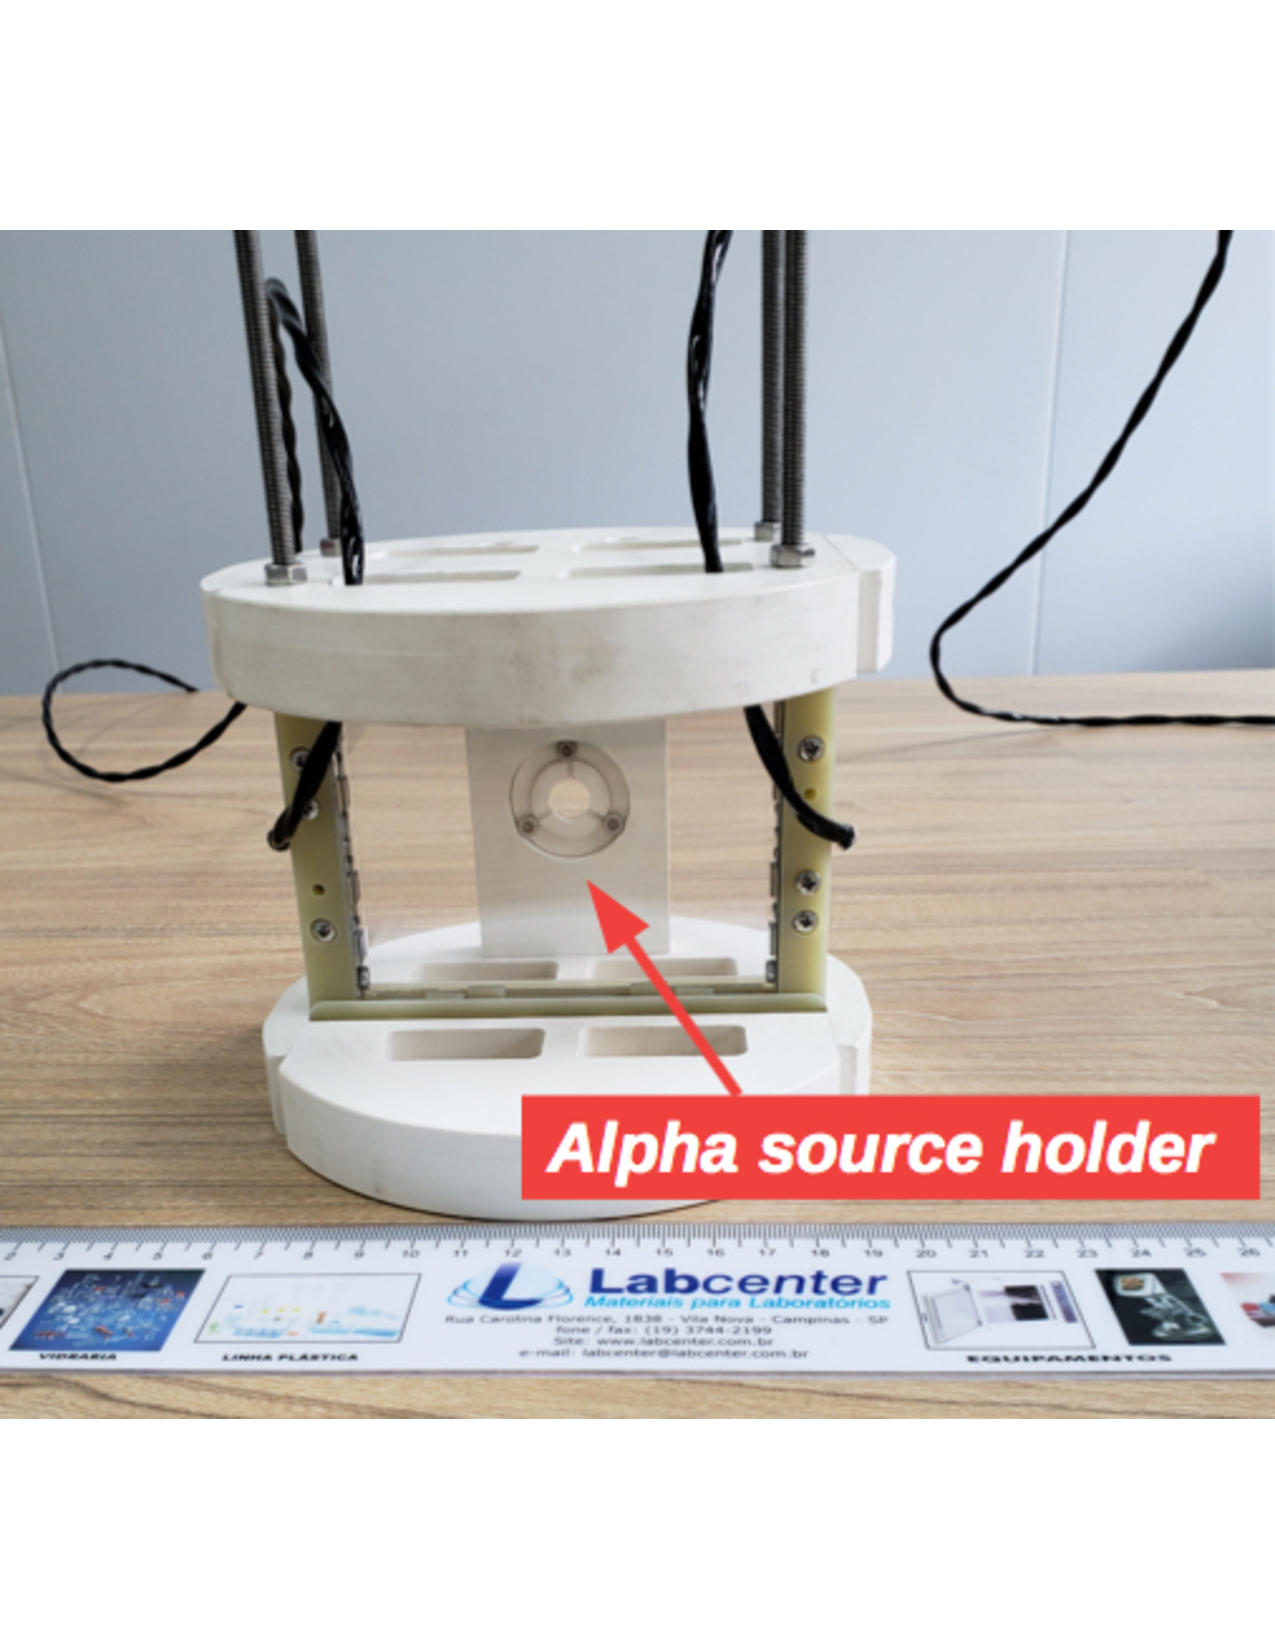
\includegraphics[height=7cm]{pds-unicamp-sample-cell-holder}
\end{dunefigure}  

The stainless-steel cylinder  is deployed in a small open dewar which is filled with commercial LAr to act as a thermal bath. In order to achieve the highest possible LAr purity inside the \dword{xarapu} chamber, the cylinder was pre-baked and vacuum pumped down to a pressure of \SI{e-5}{mbar}  %\SI{10$^-5$}{mbar} 
prior to filling it with pure argon (grade 6.0). The level of the liquid was monitored with a level meter and was set to an height able to submerge completely bot the alpha source and the \dword{xarapu}. 

The alpha source was exactly the same used in the ARAPUCA proof-of-principle tests detailed in Section~\ref{sec:proof-principle}, that is an alloy of natural uranium and aluminium in the form of a metallic disc of \SI{1}{cm} diameter and \SI{150}{$\mu$m} thickness emitting three alpha lines with energies of  \SI{4.187}{MeV}, \SI{4.464}{MeV} and  \SI{4.759}{MeV} with relative abundances of 48.9\%, 2.2\% and 48.9\% respectively.  The electronic read-out chain is composed by a custom pre-amplifier (gain $\sim$ 10) and by a commercial CAEN DT5720 desktop digitizer\footnote{https://www.caen.it/products/dt5720/}.

\begin{dunefigure}[Single photon spectrum and alphas’ energy spectrum.]{fig:xarapu-results}
{Reconstructed single photon spectrum (left). The spectrum is fitted with a multi-gaussian to take into account for the electronic noise peak, the one and multiple photons signals. The  spectrum of the total number of photo-electrons collected with the alpha source (right) is shown with a black line. The red line is a fit with an analytic description of the spectrum (see text).} 
	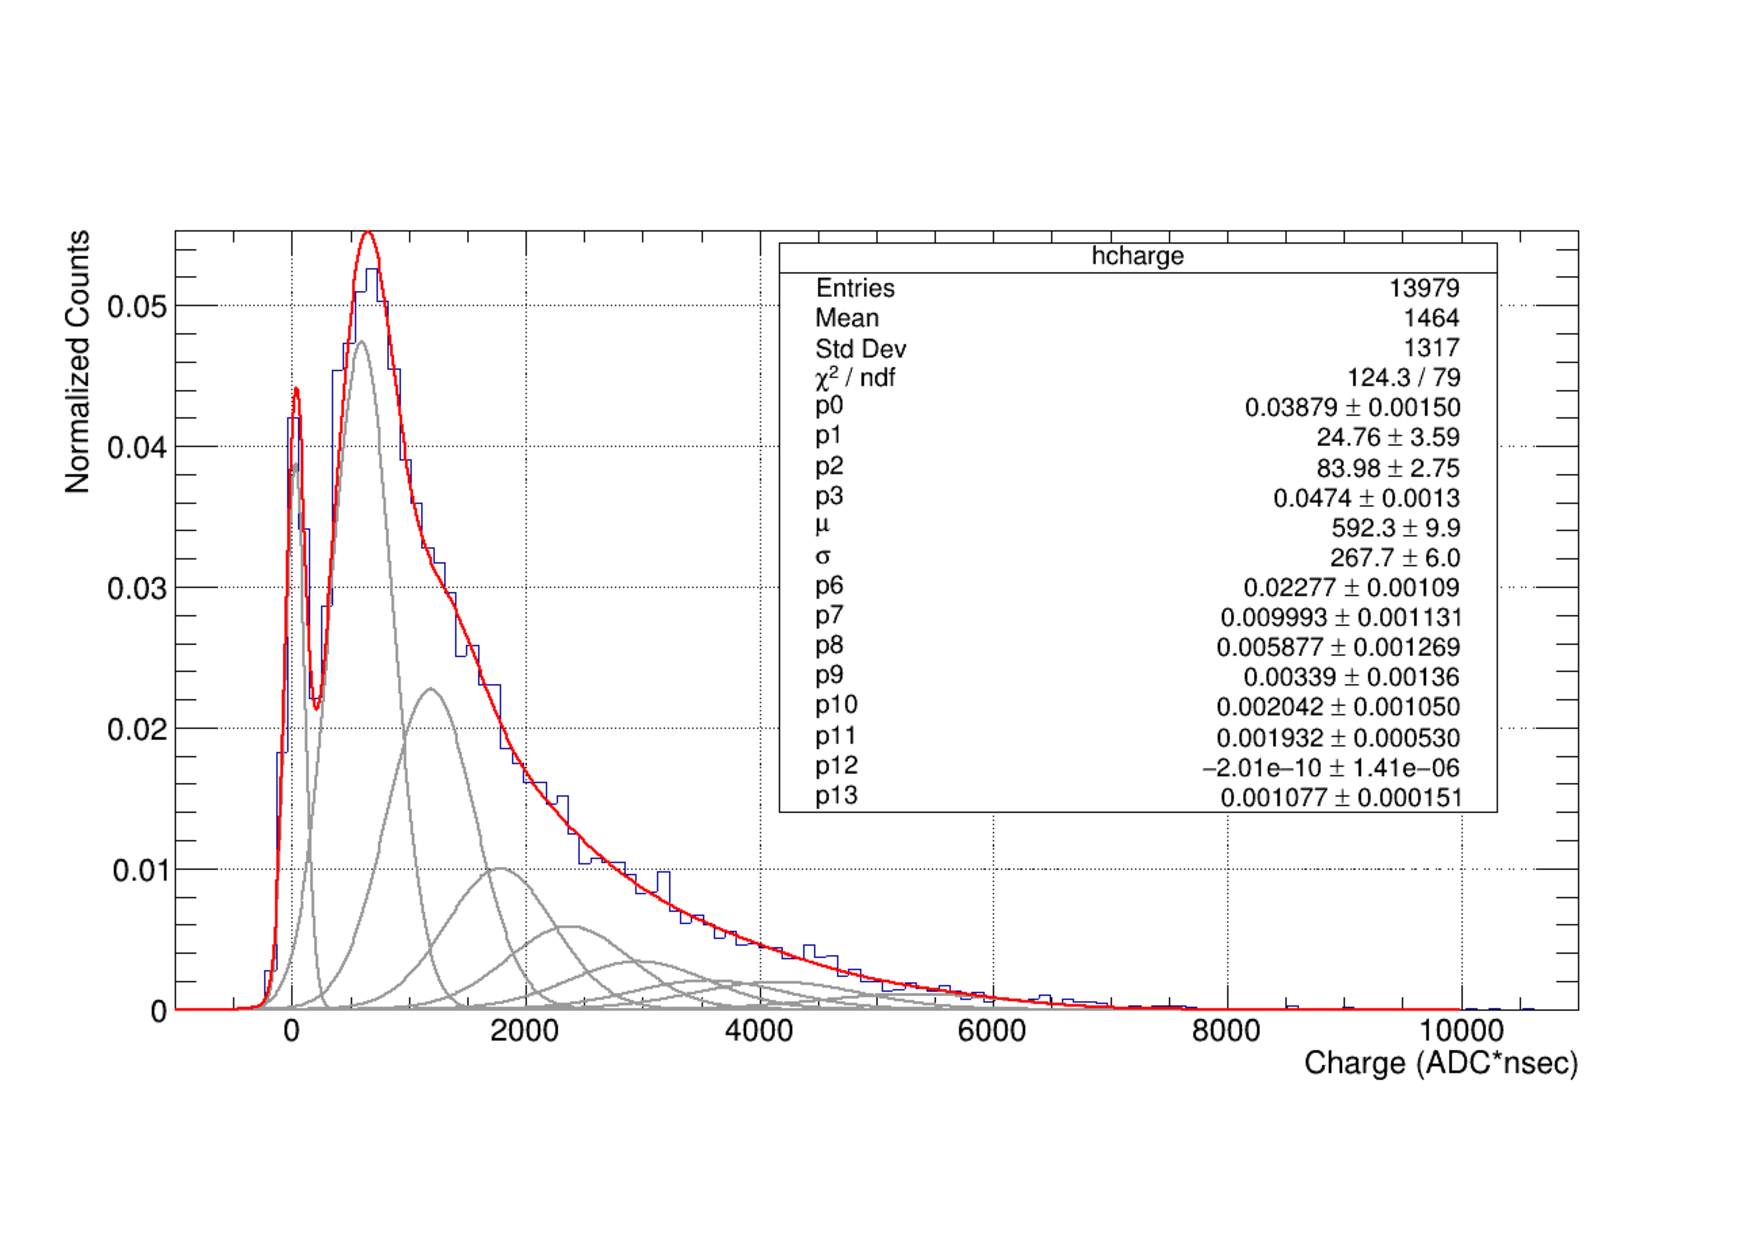
\includegraphics[height=6cm]{pds-sphe-fit-nolog} \quad
	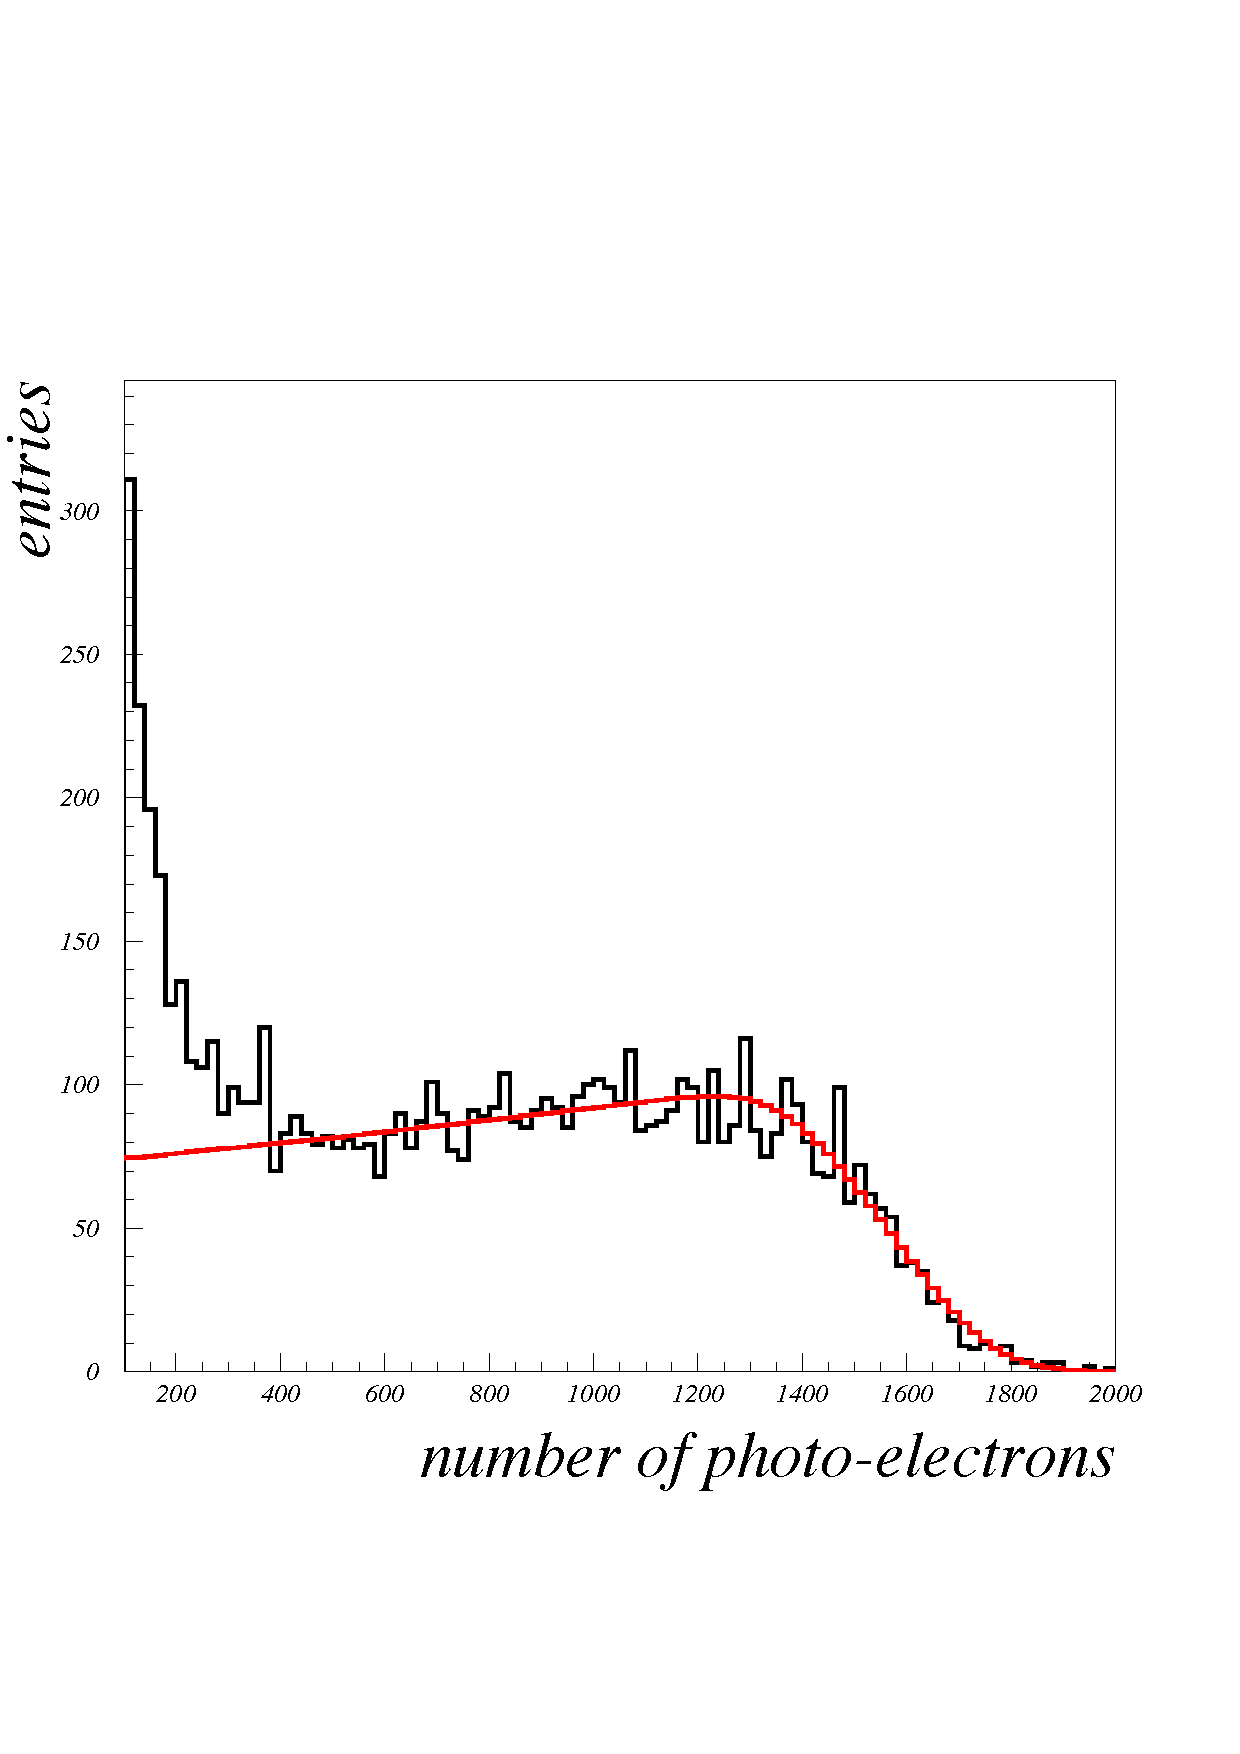
\includegraphics[height=7cm]{pds-spectrum-fitted-double}
\end{dunefigure}  


The waveforms detected by the two SiPM arrays are integrated for \SI{10}{$\mu$s}, converted into photo-electrons and summed. 
The single photo-electron spectra are reconstructed by searching for single photon peaks in  the tail of the recorded waveforms starting from about \SI{15}{\micro\second} from the onset of the scintillation signal. The selected peaks are integrated for \SI{600}{ns} to determine the associated charge. The single \phel spectrum for one of the channels is shown in figure \ref{fig:xarapu-results}, left. The resolution of the single and multi-photon peaks is fairly poor mainly because  four \dwords{sipm} are passively ganged together and because the gain of the pre-amplifier is relatively small. Three different analysis techniques for the extraction of the single \phel spectrum have been implemented and all of them pointed towards the same results.

The spectrum of the detected number of photons is shown in Figure~\ref{fig:xarapu-results}, right with a black line. The same fit procedure adopted for the ARAPUCA proof-of-principle tests allows to estimate the number of detected photons for each alpha line. The result of the fit is shown with a red line in Figure~\ref{fig:xarapu-results} and returns a number of photo-electrons of $\sim$ 1600 of photo-electrons for the reference alpha line at \SI{4.187}{MeV}. The efficiency is estimated by calculating the number of scintillation photons impinging on the \dword{xarapu} window for the relative alpha line, considering that the source can be well approximated as being point like (the range of \SI{5}{MeV} alphas in \lar is \SI{30}{\micro\meter}) and that the fraction of the solid angle covered by the \dword{xarapu} window is about 0.2. A more precise estimation  will be done with  a detailed Monte Carlo simulation of the entire experimental set-up, which takes into account the optical properties of all the internal surfaces and materials (e.g., shifting film, filter(s), wavelength shifting plate, internal reflector, stainless-steel internal surfaces).  The total detection efficiency results to be $\SI{4.7\pm0.8}{\%}$. Afterpulses and crosstalk have not been considered.



%[Note in 1st draft:  In the coming weeks, absolute detection efficiencies for the double sided readout \dword{xarapu} configuration will be extracted using data collected in these initial tests.  Additional other tests will be performed, including single sided \dword{xarapu} tests (with a Vikuiti reflective foil installed on the non-viewing side of the test cell in place of one of the dichroic window), as well as single- and double-sided \dword{sarapu} configurations, allowing for a complete suite of comparisons of detector performance.]



% 
%%%%%% rjw edits, ZD edits

\subsection{ICEBERG Test Stand}
\label{sec:iceberg-teststand}
%\fixme{summary of what PD is going into ICEBERG needed and schedule for when we might expect \dword{xarapu} results}
%\fixme{Description of ICEBERG (described in other chapters? electronics?) and the arapucas that will be in.}
%fixme{Iceberg section added here.  Comments?}
%\fixme{Integrate the mention of Mu2e electronics text from Josh pasted at the end of this section.}

The ICEBERG test-stand is a small-scale TPC using reduced-size \dword{fd} \dword{apa} and cathode designs constructed primarily to provide a platform for DUNE \dword{ce} testing at \dword{fnal}. 
The test stand consists of an approximately \SI{94.7}{cm} $\times$ \SI{79.9}{cm} anode plane assembly, with an approximately \SI{30}{cm} drift length from a cathode plane on each side.  
It can accommodate up to two almost 1/2-length \dword{pd}\footnote{In order to use existing \dword{apa} components from \dword{pdsp} as a cost-saving measure, however, slight modifications were made to the \dword{apa} frame resulting in \dword{pd} modules \SI{50}{mm} shorter than final modules will be, requiring slight modifications to the \dword{pd} module design.} in a mounting structure nearly identical to the final DUNE FD configuration, allowing for testing of \dword{pd} prototype performance, electrical connections, and interfaces with the \dword{ce} and \dword{apa} systems. 
In addition, it will be used to allow comparisons between Mu2e-based warm electronics and \dword{pdsp} \dword{ssp} system, as well as testing newer versions of photosensors active ganging circuit designs.

%The photos are nice but not directly germane to the PD tests.
%Figure~\ref{fig:fig-iceberg} shows the ICEBERG TPC. 

The ICEBERG facility will enable the primary validation of the \dword{xarapu} design prior to a full-scale test envisioned at a future \dword{pdsp} run in 2020. 
%It is envisioned that up to three test cycles will be performed prior to the DUNE technical design report submission.
At least two test campaigns are planned for the ICEBERG TPC with PD modules:  An initial test run in December 2018 incorporated one full-length \dword{sarapu} supercell and one full-length \dword{xarapu} supercell.  Both of these supercells incorporate single-sided readout, allowing comparisons of \dword{sarapu} and \dword{xarapu} performance to summer and fall 2018 \dword{pdsp} measurements.

%\begin{dunefigure}[zd more ICEBERG figures all together.]
%{fig:fig-iceberg}
%{ICEBERG cryostat (left figure). ICEBERG signal feed-through (right figure). }
%\includegraphics[angle=0,width=7cm,height=5cm]{ICEBERG_0.png}
%\includegraphics[angle=0,width=7cm,height=5cm]{ICEBERG.png}
%\end{dunefigure}

 \begin{dunefigure}[ICEBERG TPC Model and assembled \dword{apa}.]
 {fig:fig-pds-iceberg-tpc}
 {Software solid model of ICEBERG TPC (left), and assembled ICEBERG \dword{apa} (right).  Note the \dword{pd} module mounting rails, which are vertical in this image but horizontal in operation. The centrally-mounted \dword{apa} allows for testing of double-sided readout photon detector modules.}
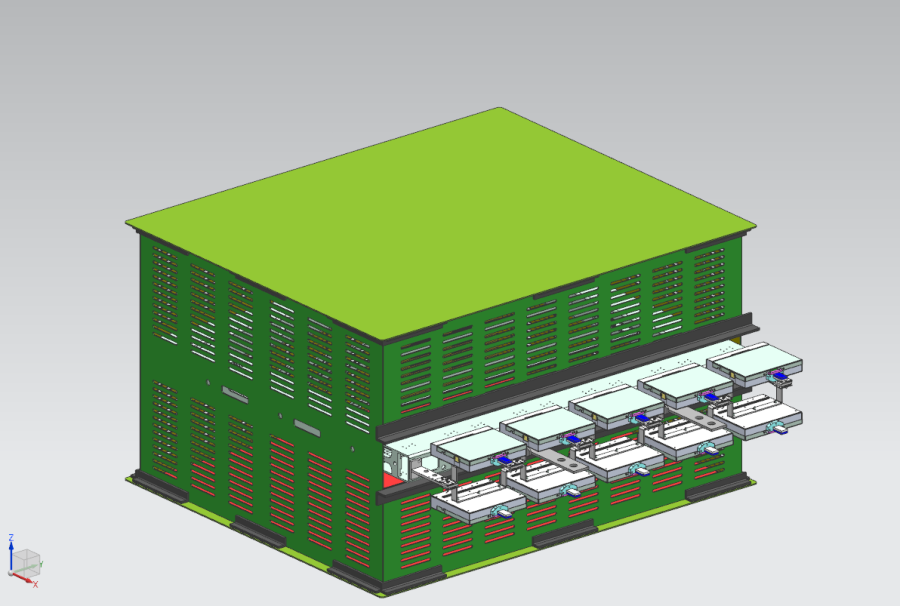
\includegraphics[angle=0,width=8.4cm,height=6cm]{pds-iceberg-tpc}
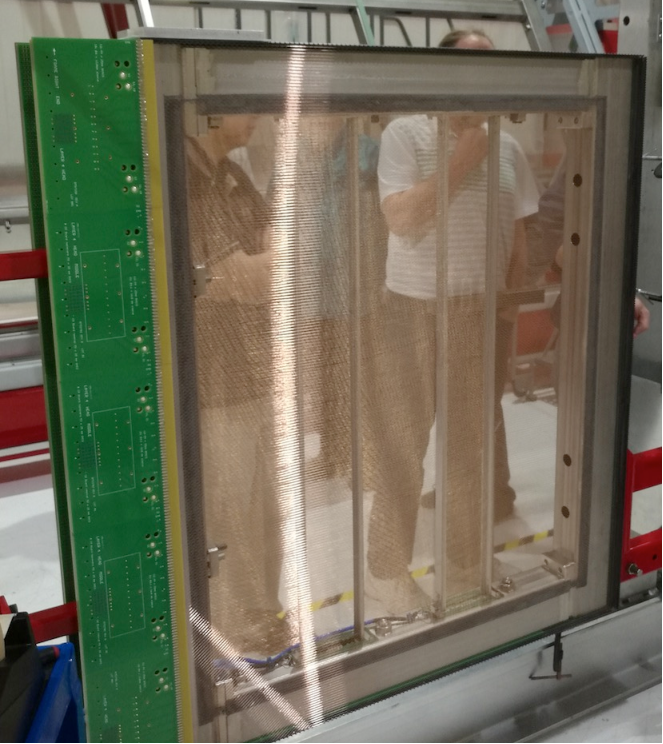
\includegraphics[angle=0,width=8.4cm,height=6cm]{pds-iceberg-apa.pdf}
\end{dunefigure}

%Since the \dword{apa} for the ICEBERG test stand is nearly half the width of a full far-detector \dword{apa} frame, including full-size PD insertion slots (\SI{136}{mm}$\times$\SI{25}{mm}) and electrical connections.  


\begin{dunefigure}[Single-supercell ICEBERG PD module.]
 {fig:fig-pds-iceberg-tpc}
 {Software solid model of single-supercell ICEBERG PD module (left) and fabricated components during assembly (right).  Note connector board (green) in right photo is mounted to the \dword{apa} frame prior to wire wrapping.}
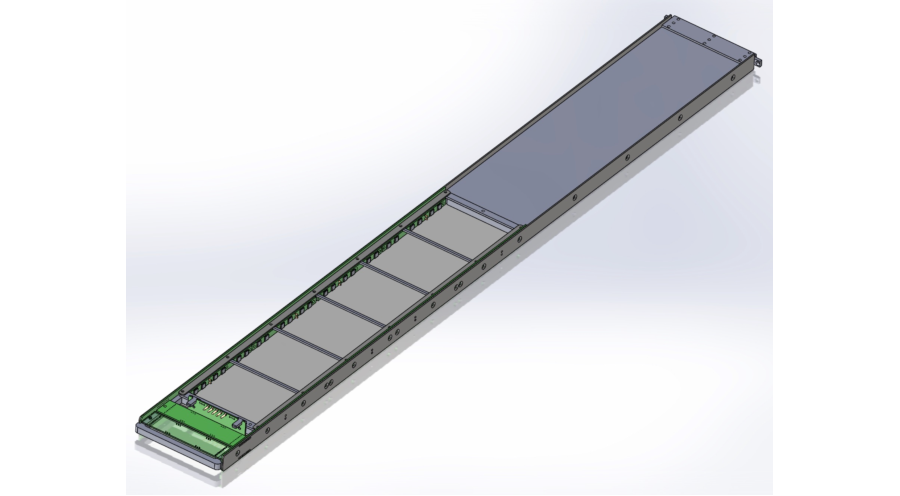
\includegraphics[angle=0,width=8.4cm,height=6cm]{pds-iceberg-run-1-module.pdf}
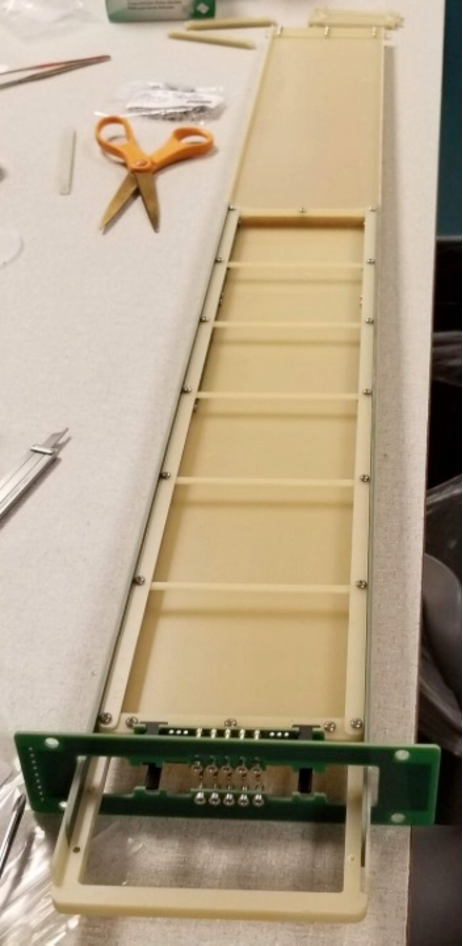
\includegraphics[angle=0,width=8.4cm,height=6cm]{graphics/pds-iceberg-module-assembly-photo.pdf}
\end{dunefigure}

A second campaign is planned for winter/spring 2019, incorporating two \dword{sarapu} and two \dword{xarapu} supercells, partially occluded in the frame due to the limitations in \dword{apa} size mentioned above.  One supercell of each kind will be single-sided and one double-sided, allowing for additional comparisons of \dword{pd} technologies.

Along with the \dword{pds} technology studies, the test stand will  provide further testing and validation of the \dword{pds} Mu2e-based electronics system, including a side-by-side comparison with the \dword{pdsp} \dword{ssp} electronics readout. In addition, concurrent data taking with the TPC and light collection system will allow us to study TPC-induced noise on the \dword{pd}, \dword{pd}-induced noise on the TPC, grounding scheme configuration, controller-\dword{daq} and controller-\dword{feb} interfaces, bandwidth and rates issues, online and offline \dword{pd}-TPC interfaces, zero-suppression techniques, firmware development, accepting and producing triggers, and, in general, will inform possible upgrade paths for the system. 


%%%%%%%%%%%%%%%%%%%%%%%%%%%%%%%%%%%%%%%%%%%%%%%%
% Provided by dj 11/26/18
\subsection{Calibration and Monitoring}
\label{sec:fdsp-pd-validation-candm}

%\metainfo{Content: Djurcic}

All major components of the \dword{spmod} \dword{pds} calibration and monitoring system have been designed, fabricated, tested, and operated in \dword{pdsp}.
Figure~\ref{fig:pds_calmon_fig2} shows the hardware components of the system.

 \begin{dunefigure}[\dword{pdsp} UV calibration and monitoring system.]
 {fig:pds_calmon_fig2}
 {The figures show the hardware components of the \dword{pdsp} calibration and monitoring system.}
 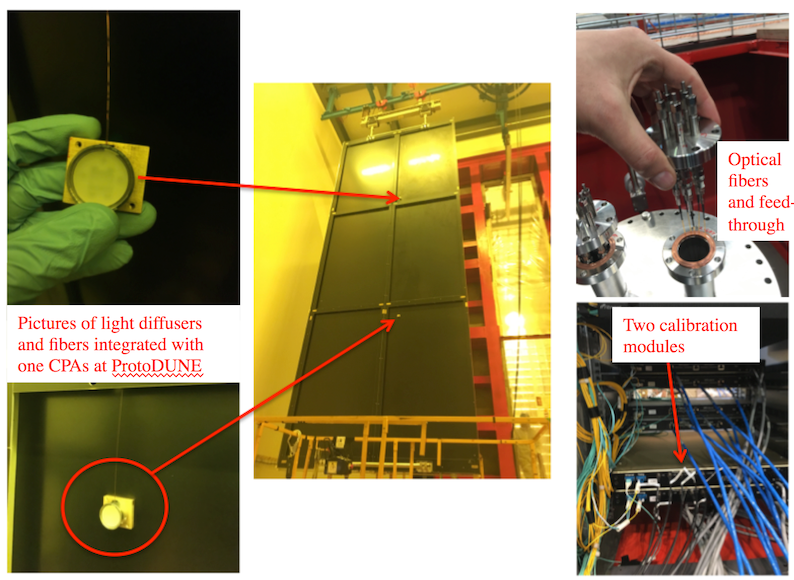
\includegraphics[angle=0,width=11.4cm,height=9cm]{graphics/pds-calmon-fig2.png}
\end{dunefigure}

Although at a longer wavelength than \lar scintillation light, the UV light from the system exercises the full chain of measurement steps initiated by a physics event in the \dword{detmodule}, starting from the wavelength %-shifter 
conversion, photon capture in the \dword{xarapu}, photon %sensor 
detection and the \dword{fe} electronics readout.
Figure~\ref{fig:pds_calmon_fig3} shows typical double waveforms recorded by an \dword{pdsp} \dword{ssp} module as a response to calibration system
light pulses illuminating %one of ARAPUCA 
an \dword{sarapu} channel. Here, the calibration modules and \dwords{ssp} are triggered externally through the trigger and timing system to efficiently collect calibration light pulses  and minimize rate of in-time cosmic ray muons.

 \begin{dunefigure}[\dword{pdsp} ARAPUCA response to UV calibration and monitoring system.]
 {fig:pds_calmon_fig3}
 {Double waveforms recorded by \dword{pdsp} \dword{ssp} module as a response to calibration system light pulses collected by an \dword{sarapu} channel.}
%\fixme{Zelimir: Can the plot be made with a smaller y-axis scale to reduce the white space?}
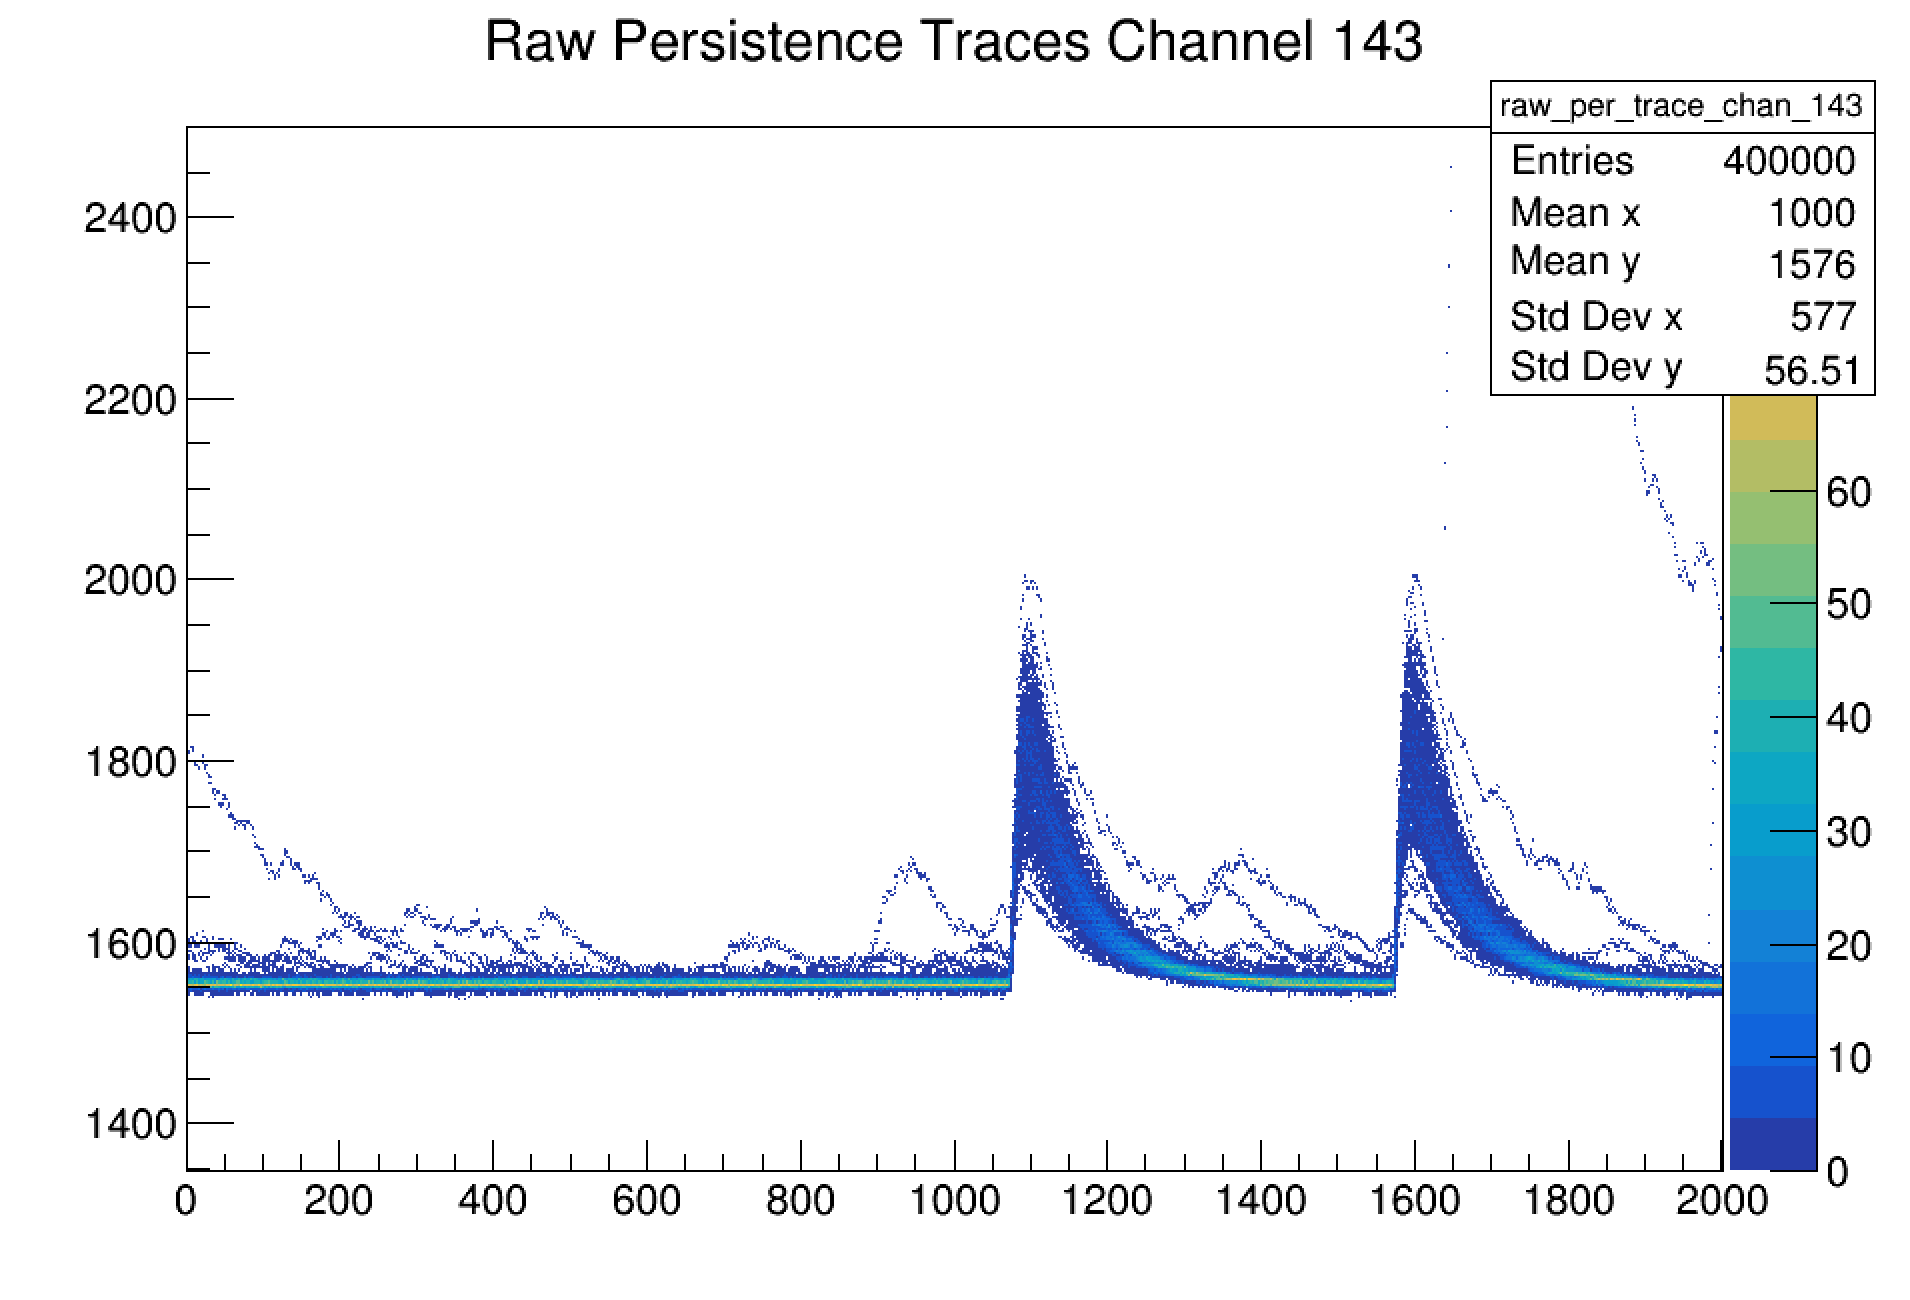
\includegraphics[height=4cm]{graphics/pds-calmon-example.png}
\end{dunefigure}

The \dword{pdsp} data set has been collected and the data analysis is underway.
Goals of the analysis are to verify that the \dword{cpa} includes % there is 
an optimal distribution of light diffusers for the \dword{spmod};  %at the \dword{cpa} for DUNE; use the system 
to evaluate gain and timing resolution; to perform relative comparisons of photon channels;
and to characterize and monitor stability of the \dword{pds} over the duration of \dword{pdsp}. The results will inform the design of an optimal
\dword{pds} calibration and monitoring plan for the \dword{spmod}.%DUNE.

\subsection{Materials Selection, Testing and Validation}

\subsubsection{PD Module Mechanical Frame}

The APA mechanical frame components are fabricated from FR-4 G-10 (garolite), a glass-epoxy laminate commonly used in printed circuit boards and other mechanical applications where an electrically insulating component with low thermal expansion coefficient is required.  G-10 is widely used in cryogenic applications, including most of the other \dword{dune} subsystems (See \citedocdb{10462} for an extensive discussion in the context of the HV system cathode planes). 

As shown in table \ref{tbl:fdsfpdshrink}, the thermal contraction of FR-4 is closely matched with that of stainless steel, simplifying design of the module interface with the \dword{apa} frame.

Selecting FR-4 as our main module mechanical material comes at some cost in additional difficulty machining, but allow  allows us to use long printed circuit boards for routing photosensor electrical signals along the detector sides without incurring thermal expansion issues.  As an excellent insulator, FR-4 also simplifies electrically isolating the PD system from the APA frame, as required by the \dword{dune} grounding scheme.

FR-4 has been certified at the \dword{fnal} materials test stand as an acceptable material for use in \dword{dune} from the standpoint of \dword{lar} contamination.

All fasteners used in the \dword{pd} are stainless steel alloy 304, widely used in cryogenic applications.  This alloy has also been certified at the \dword{fnal} materials test stand as an acceptable material for use in \dword{dune} from the standpoint of \dword{lar} contamination.

\subsubsection{\dword{pd} Module-\dword{apa} Frame Mechanical Support Structure}

All \dword{pd} mechanical supports (including rails, brackets and fasteners are to be manufactured from stainless steel alloy 304.  This has the benefit of matching thermal contraction coefficients with the \dword{apa} frame and being approved for use in \dword{lar} by the materials test stand.

\subsubsection{Dichroic Filter/Filter coating}

The dichroic filters used in \dword{xarapu} consist of a fused silica substrate, coated on one face to provide the required dichroic properties and on the opposite face with a thin evaporated layer of pTP.

Fused silica was selected in part due to its excellent low-temperature properties.  It is widely used as an optical window in low temperature, due to it's stability and low coefficient of thermal contraction, and fused silica dichroic filters have performed well in many ARAPUCA validation tests.

Testing of the pTP coating is of greater concern.  Initial validation of the \dword{sarapu} in \dword{tallbo}, \dword{pdsp} and in repeated cryogenic immersion tests at \dword{fnal} and other facilities has demonstrated that while it is possible to generate highly-reliable pTP coatings on fused silica substrates, careful surface preparation and deposition procedures are required to prevent catastrophic failure of the coating.  In addition, further studies of diffusion of trace amounts of pTP into the \dword{lar} will also be beneficial.  To facilitate this work,  Syracuse University is developing a test stand to investigate the long-term stability of \dword{xarapu} optical coatings in liquid argon. Dissolution of similar wavelength-shifting coatings into liquid argon has been recently observed in a technology-dependent fashion (1), so investigation of the designs specific to \dword{dune} is necessary to confirm their robustness. Subjecting coated materials to a continuous flow will also stress the adhesion of the coating to the plates to simulate the convective flow of liquid argon in the far detector cryostat.

The test stand will consist of a \SI{74}{L} liquid argon cryostat. Coated filters and related detector elements will be suspended in a continuous flow of liquid argon and periodically inspected for degradation in their response. A vacuum-ultraviolet monochromator and a dark box containing a visible-light scanning bed will measure wavelength shifting performance of the tested elements before and after suspension within the argon flow.

\fixme{add Denver's pictures here}

Commissioning is planned for early 2019, with a measurement program to inform component production optimization running through late 2019. This test stand will also facilitate future contributions from Syracuse University to the field of liquid argon detector research and development.

\fixme{Dave- how do I enter this reference? [1] J. Asaadi, B. J. P. Jones, A. Tripathi, I. Parmaksiz, H. Sullivan, and Z. G. R. Williams. Tetraphenyl Butadiene Emanation and Bulk Fluorescence from Wavelength Shifting Coatings in Liquid Argon. 2018. arXiv:1804.00011.}
\fixme{Dave - Use \cite{Asaadi:2018ixs} (from anne this is in bib file)- I didn't know where you want it.  rjw}


\subsubsection{\dword{wls} plates}

The \dword{xarapu} wavelength shifting plates are fabricated by the same vendor as the light guide bars utilized in the double-shift \dword{pdsp} modules.  The \dword{xarapu} \dword{wls} plates are made with the same transparent matrix material, but have a different wavelength shifting dopant added.  

While it is possible that the cryogenic properties of this modified \dword{wls} material may be altered by the change in doping agent, it is expected that the tests done for the double-shift bar prototypes are a valuable guide for their expected performance.  As part of the design verification, samples of these bars were manually thermocycled to verify they didn't craze. In addition, we used the Indiana University, USA \lar test stand with an alpha source behind a small sample of the \dword{wls} plate to scan the attenuation length of a short sample. Finally, we built a long darkbox with a $\sim\,$\SI{420}{nm} LED scanning down the length of a full bar to verify its attenuation length and compare to the LAr data. (This is what formed the basis of the threshold requirements on in-air attenuation length for the ProtoDUNE batch.) 
This same sequence will be undertaken for the light guides selected for \dword{xarapu}. As with most other components, it is not possible to simulate long-term exposure to \dword{lar} of a length similar to that expected in \dword{dune}, so we will substitute by testing repeated thermal cycling to maximize thermal stresses in the material.  Finally, samples of the \dword{wls} plates will be certified for use in \dword{dune} in the the materials test stand at \dword{fnal}.  

